\documentclass{sig-alternate}
\usepackage{etoolbox}
\makeatletter
\patchcmd{\maketitle}{\@copyrightspace}{}{}{}
\makeatother

\usepackage[caption=false]{subfig}
\usepackage{verbatimbox}
\providecommand{\e}[1]{\ensuremath{\times 10^{#1}}}
\usepackage{enumitem}




\begin{document}

\title{Randomized Optimization, Unsupervised Learning, and Dimensionality Reduction}
\subtitle{Writeup for Assignment 02 - CS 6741}

\author{
\alignauthor
Magahet Mendiola
}
\date{}

\maketitle
\begin{abstract}
An empirical analysis of randomized optimization, clustering, and dimensionality reduction algorithms.
\end{abstract}

\section{Part 1: Randomized Optimization}

In order to compare and contrast the given randomized optimization algorithms, a classification task was taken from the previous assignment and each algorithm was utilized to train a neural network to perform this task. Implementation of each algorithm as well as the code for running the neural network was taken from the ABAGAIL machine learning library (https://github.com/pushkar/ABAGAIL).

\subsection{Neural Network Training}

\paragraph{Classification Task}

The dataset used to test our neural network optimization task was the Adult dataset from the UCI repository. This was the second of the two classification datasets used in the supervised learning assignment. To recap, these are samples of personal socioeconomic attributes with a binary classification of gross net income over or below 50k/yr.

This dataset should prove interesting as an optimization task, since we have a fairly clear intuition of the relationship between the attributes and the classifications. From the previous assignment, we could see that attributes such as capital gain or loss had a strong linear relationship to the classification, as did education level. Intuition, or in this context domain knowledge, suggests that the fitness function for our neural network will have a smooth surface with predictable gradients. This is due to belief that having a slightly higher or lower education level would have a slightly higher or lower (mostly predictable) impact on one's net worth. In the case of our neural network, the actual fitness function is the sum of squared errors between the network's output and the actual instance binary values.

The optimization task was run against a training set of 1,000 instances from the adult dataset and final classification error was then measured with a separate testing set of another 1,000 instances. 19 attributes were used from the set and nominal attributes were first converted into separate binary attributes.

\paragraph{Optimization Parameters}

Randomized hill climbing, simulated annealing, a genetic algorithm, and gradient decent were all utilized to train the weights for our neural network. The network consisted of 19 input nodes, 5 hidden nodes, and 1 output node. Each algorithm was given 1,000 training iterations to find an optimum set of weights. Simulated annealing was set with an initial temperature of 1\e{11} and a cooling exponent of 0.95. The genetic algorithm used a population of 200 with a set of 100 used for crossover and another 10 used for mutation.

\paragraph{Optimization Results}

Using three randomized optimization algorithms, our neural network was trained over 1000 iterations each. The classification accuracy of each of these trained networks is shown in Figure~\ref{ann-error-summary}. As shown, randomized hill climbing outperformed the rest both in terms of training the network to correctly classify instances and in the time required to train the network. Simulated Annealing was negligibly faster, but the resulting network did not perform as well in the classification task.

\begin{verbbox}
Results for RHC: 
Correctly classified 764.0 instances.
Incorrectly classified 236.0 instances.
Percent correctly classified: 76.400%
Training time: 3.709 seconds
Testing time: 0.004 seconds

Results for SA: 
Correctly classified 733.0 instances.
Incorrectly classified 267.0 instances.
Percent correctly classified: 73.300%
Training time: 3.023 seconds
Testing time: 0.004 seconds

Results for GA: 
Correctly classified 763.0 instances.
Incorrectly classified 237.0 instances.
Percent correctly classified: 76.300%
Training time: 72.068 seconds
Testing time: 0.004 seconds

Results for GD: 
Correctly classified 725.0 instances.
Incorrectly classified 175.0 instances.
Percent correctly classified: 72.500%
Training time: 6.560 seconds
Testing time: 0.004 seconds
\end{verbbox}

\begin{figure}[!htbp]
    \centering
    \theverbbox
    \caption{Randomized optimization training on ANN results\label{ann-error-summary}}
\end{figure}

This result reinforces our intuition regarding the dataset. Randomized hill climbing is similar to gradient decent in that the algorithm makes small changes in a direction that improves the fitness function result. Since we believe the profile of the adult dataset to be smooth and behaves predictably given changes in the inputs, both gradient decent and randomized hill climbing should move quickly toward a local minimum. In this case, since simulated annealing and the genetic algorithm did not find a solution that performed better than these two, we make the claim that this local minimum is in fact the global minimum.

\paragraph{Training Performance}

It is interesting to note the performance of each algorithm throughout the set of training cycles. This gives a better picture of how each optimization process interacted with the fitness function. In the case of randomized hill climbing (Figure~\ref{error-rhc}) the learning curve appears to smoothly converge toward lower classification error rates. This shows that the algorithm works well in this case in moving the fitness function step by step towards an optimum.

\begin{figure}[!htbp]
    \centering
    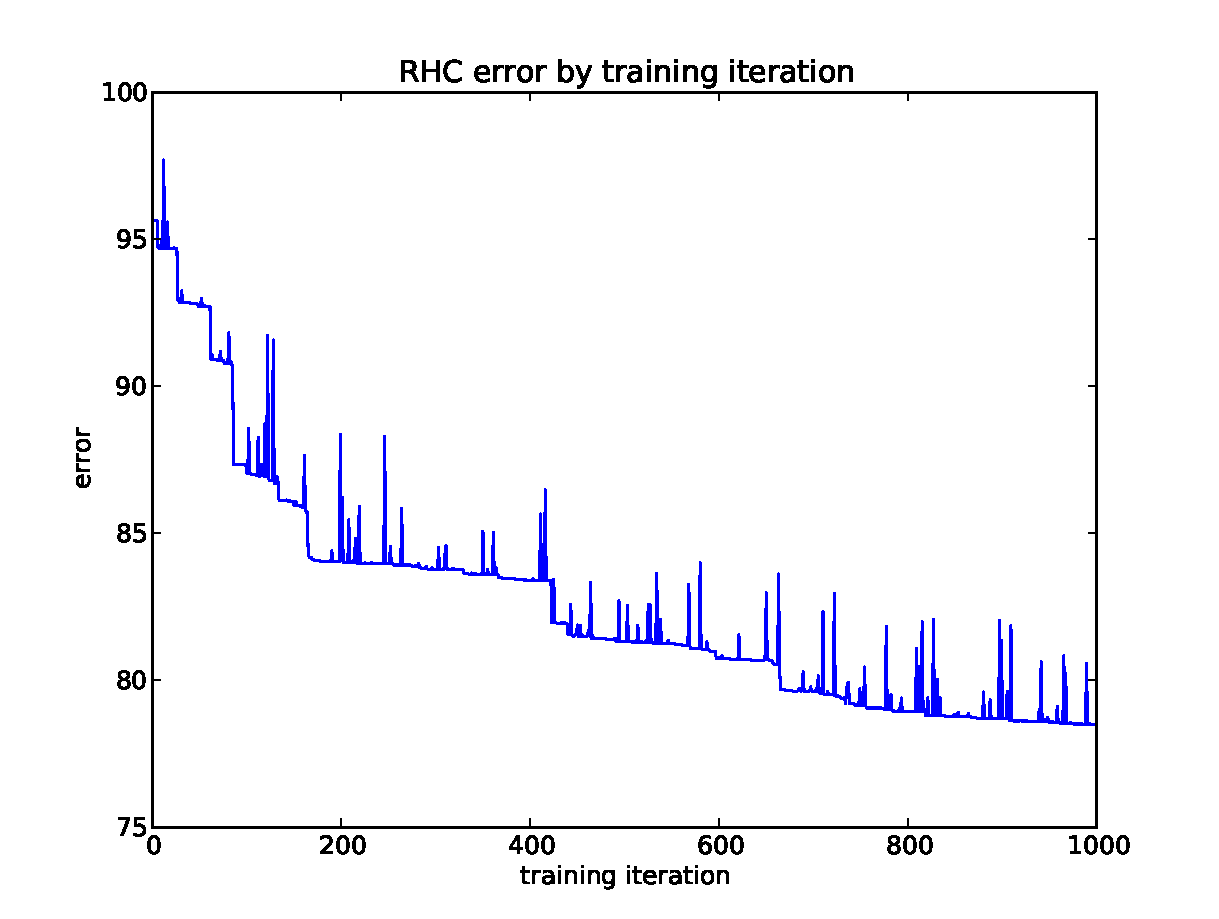
\includegraphics[width=3in]{part1.1/error-rhc.pdf}
    \caption{randomized hill climbing ANN classification error by training iterations \label{error-rhc}}
\end{figure} 

As the error rate does not seem to stabilize over the 1,000 iterations, an additional experiment was performed to see if it could continue to improve the weights if allowed to run for 10,000 iterations. The results are shown in Figure~\ref{error-rhc-10x}. You can see that the algorithm continues to find weights that result in a lower classification error on the training set. However, the resulting network resulted in almost the same classification error when run against the set aside testing set. This result illustrates the previous understanding of neural network performance and it's ability to overfit the training data.


\begin{figure}[!htbp]
    \centering
    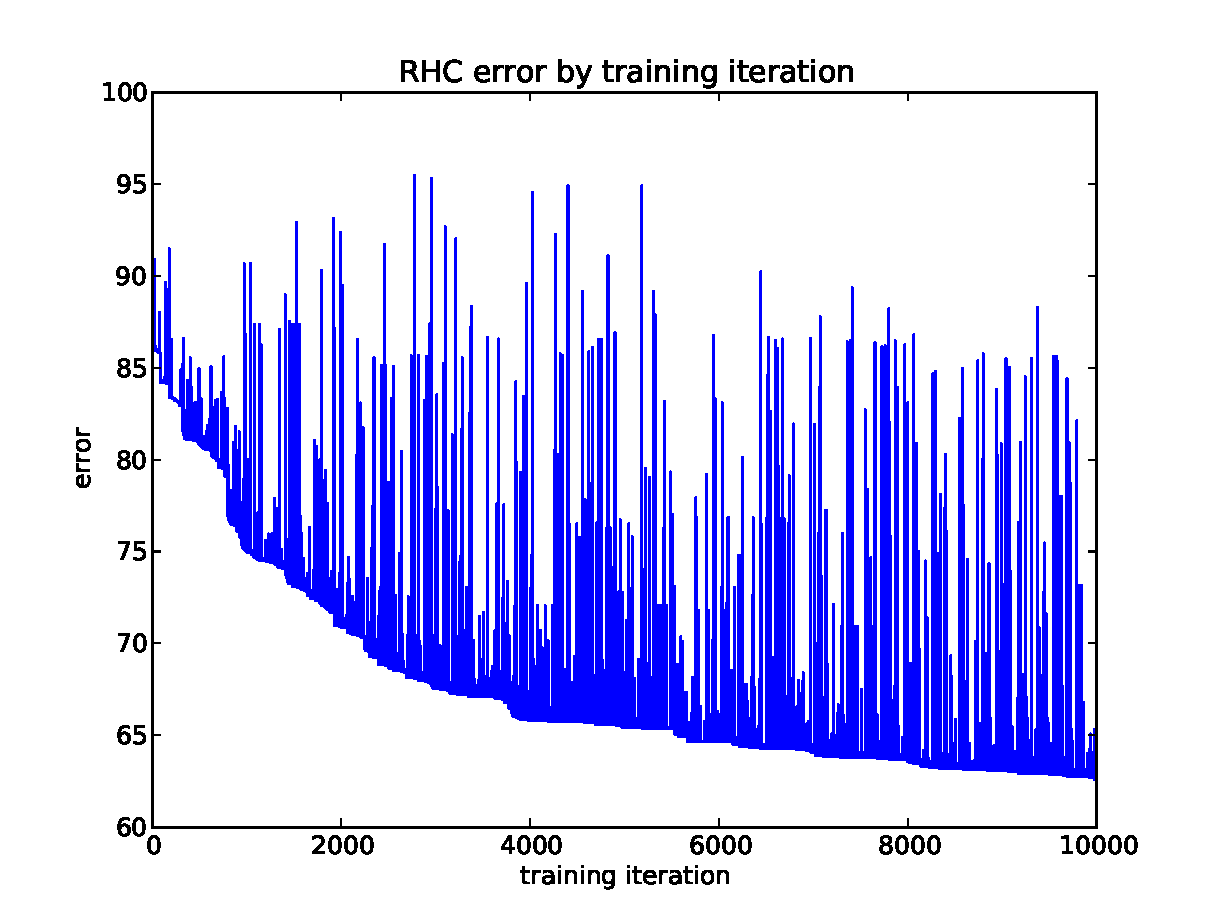
\includegraphics[width=3in]{part1.1/error-rhc-10x.pdf}
    \caption{randomized hill climbing ANN classification error by training iterations \label{error-rhc-10x}}
\end{figure} 

Figure~\ref{error-sa} shows the results of simulated annealing over the 1,000 training iterations. We see that, unlike randomized hill climbing, the error increases for more than a single iteration, and increases more towards the beginning of the process. When the algorithm fist starts, temperature is still high enough to allow movement toward less optimal results. Around 300 iterations in we see a dramatic improvement in the error. As the temperature cools, the variation in error decreases and the algorithm converges toward local optimum. In this particular optimization problem, the result of this movement in sub-optimal directions most likely caused a delay in reaching an optimal point. However, given a fitness function with a number of local optima, this behavior would have helped to discover remote valleys.

\begin{figure}[!htbp]
    \centering
    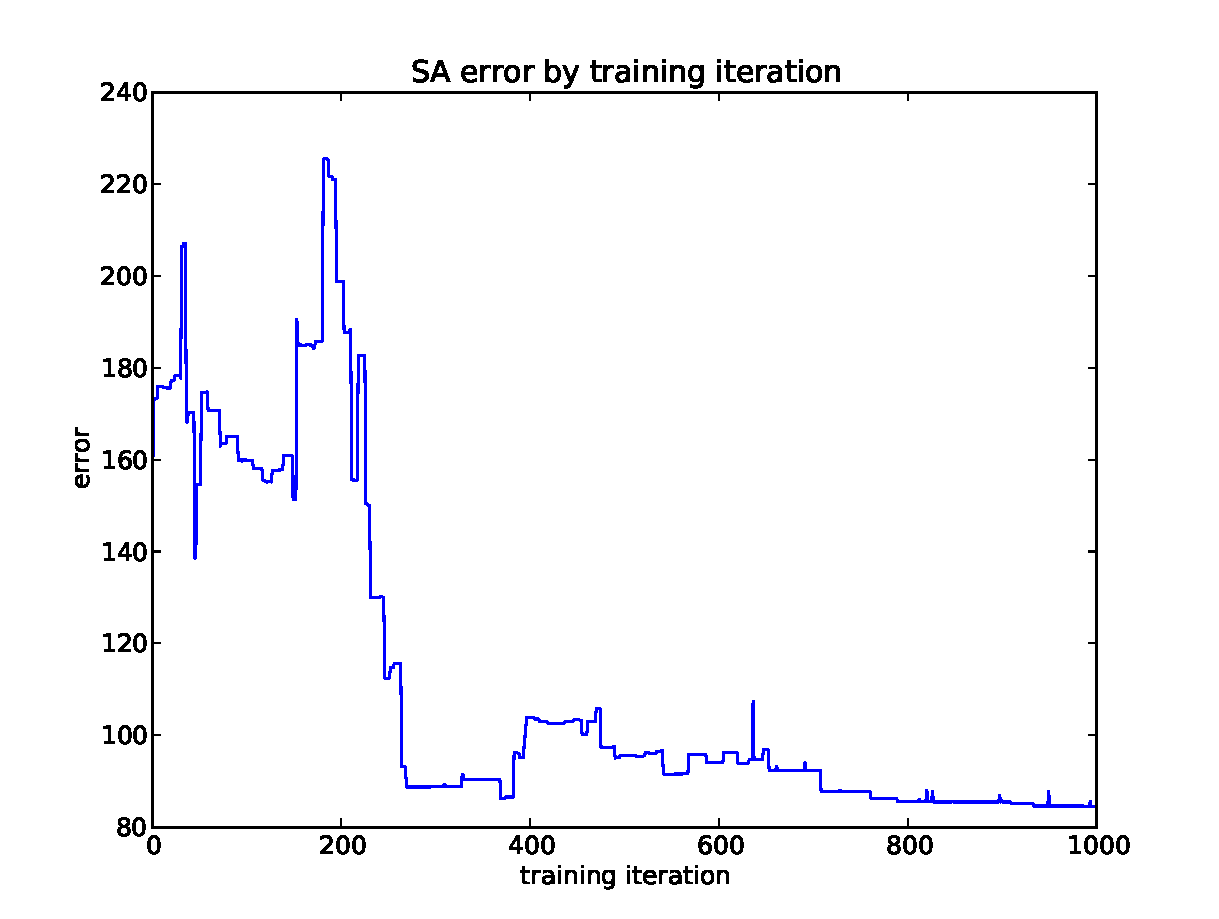
\includegraphics[width=3in]{part1.1/error-sa.pdf}
    \caption{simulated annealing ANN classification error by training iterations \label{error-sa}}
\end{figure} 

Our genetic algorithm converged very quickly toward an optimum set of weights. However, elapsed time was an order of magnitude greater than any of the other optimization algorithms. This is likely due to the computation involved in maintaining the population and performing crossover and mutation functions. This can be somewhat offset by the fact that the genetic algorithm reached a optimum set of weights in roughly half the number of iterations, but that still puts elapsed time near five times that of the others.

\begin{figure}[!htbp]
    \centering
    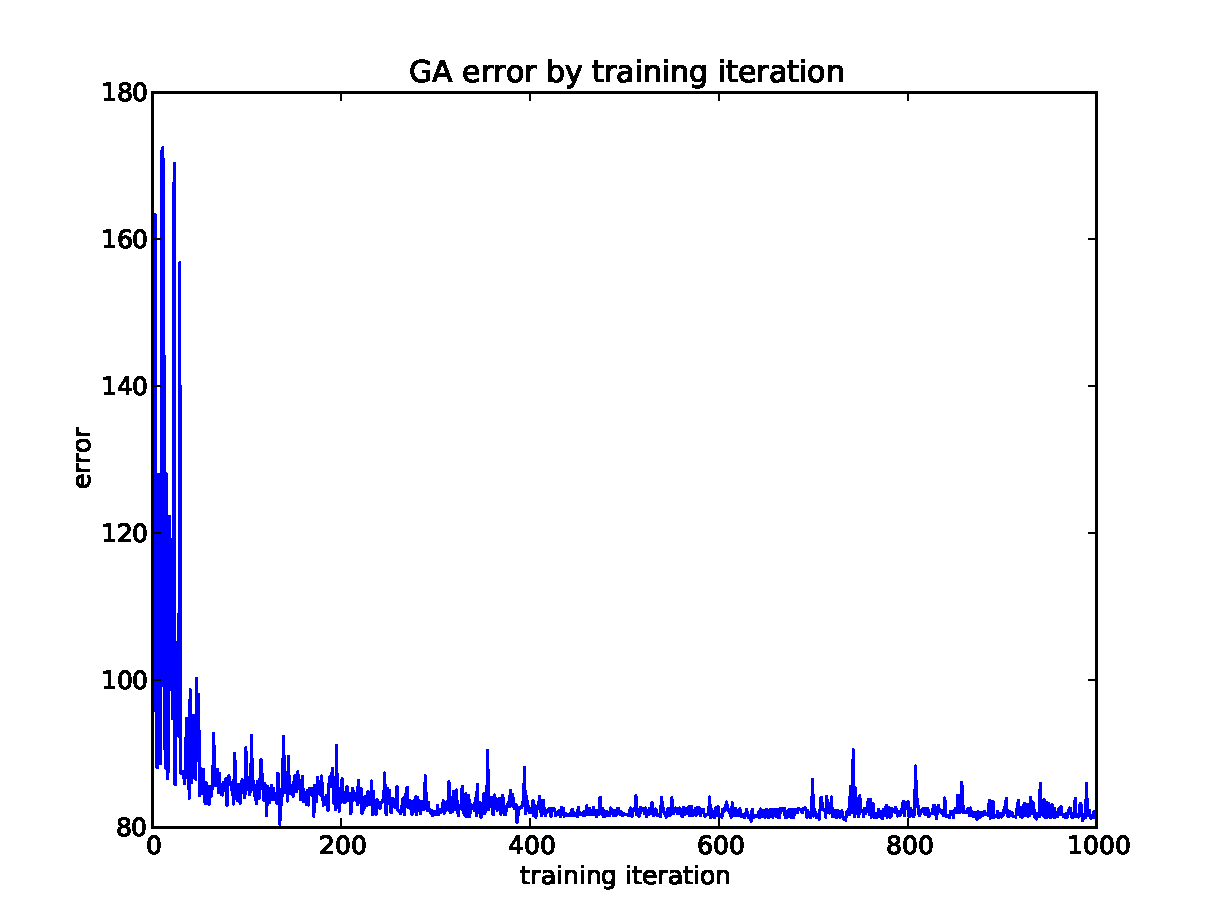
\includegraphics[width=3in]{part1.1/error-ga.pdf}
    \caption{genetic algorithm ANN classification error by training iterations \label{error-ga}}
\end{figure} 


randomized hill climbing
simulated annealing
a genetic algorithm
MIMIC

%You will then use the first three algorithms to find good weights for a neural network. In particular, you will use them instead of backprop for the neural network you used in assignment #1 on at least one of the problems you created for assignment #1. Notice that weights in a neural network are continuous and real-valued instead of discrete so you might want to think a little bit about what it means to apply these sorts of algorithms in such a domain.

\subsection{Fitness Functions}

In order to examine the properties of each randomized optimization algorithm, a number of experiments were conducted on contrived fitness functions. Each of these functions accepts an arbitrary length bit string and returns a single positive value. In order to visualize the features of these functions, they have each been plotted with the fitness score on the y axis and the input bit string encoded as a integer value on the x axis. Although this only presents a two dimensional projection of the function, it does provide some sense of behavior, including a view of local and global optima. 

For each fitness function, a series of experiments were run against each optimization algorithm. First, each algorithm was allowed to train against a fixed input space size of 80 bits. The algorithms were allowed to perform a maximum of 10,000 function evaluations before being terminated. This experiment was repeated 10 times for each algorithm and plotted to allow us to visualize the behavior of each optimization algorithm on the given fitness function as they navigated the output terrain.

The second experiment was setup to evaluate how many fitness function evaluations each algorithm required to find one of the global optima. Each algorithm was allowed to run indefinitely, until it either became stuck at a local optimum or found one of the global optima. In the former case, the algorithm was reset and re-run. This experiment was repeated for differing input space sizes (bit string lengths). The results from this set of experiments was to see how well each algorithm performed at finding the function optimum. It also provided an understanding of how well each algorithm performed given differing input sizes.

\subsubsection{Optimization Algorithm Parameters}

Each algorithm was given the same set of parameters for each experiment. 

Random hill climbing was setup to explore an input change of a single random bit and move in that direction if the fitness score improved. If an improved input was not found in a set number of evaluations (the number of input bits), the algorithm was restart with a new randomized input.

The temperature parameter for our simulated annealing algorithm was set at 1,000. This temperature was cooled by reducing it by 5\% each iteration. 

Our genetic algorithm maintained a population of 100. 50 of those were used to perform uniform bit crossover. The other 50 were mutated by swapping two random bits in their sequence.

The MIMIC algorithm was set to maintain a population of 100.


\subsubsection{Count Ones}

The count ones fitness function is well understood and easy to explain. The function simply counts the number of 1s in the input bit string. Although this is an easy heuristic to follow when calculating the function return value, the function's behavior over the input space was interesting to visualize. Figure~\ref{plot-count-ones} shows the plot of the count ones function. As we see, there are many local optima and a single global optimum. The function has a upward trend with a stair step like behavior along the way.

\begin{figure}[!htbp]
    \centering
    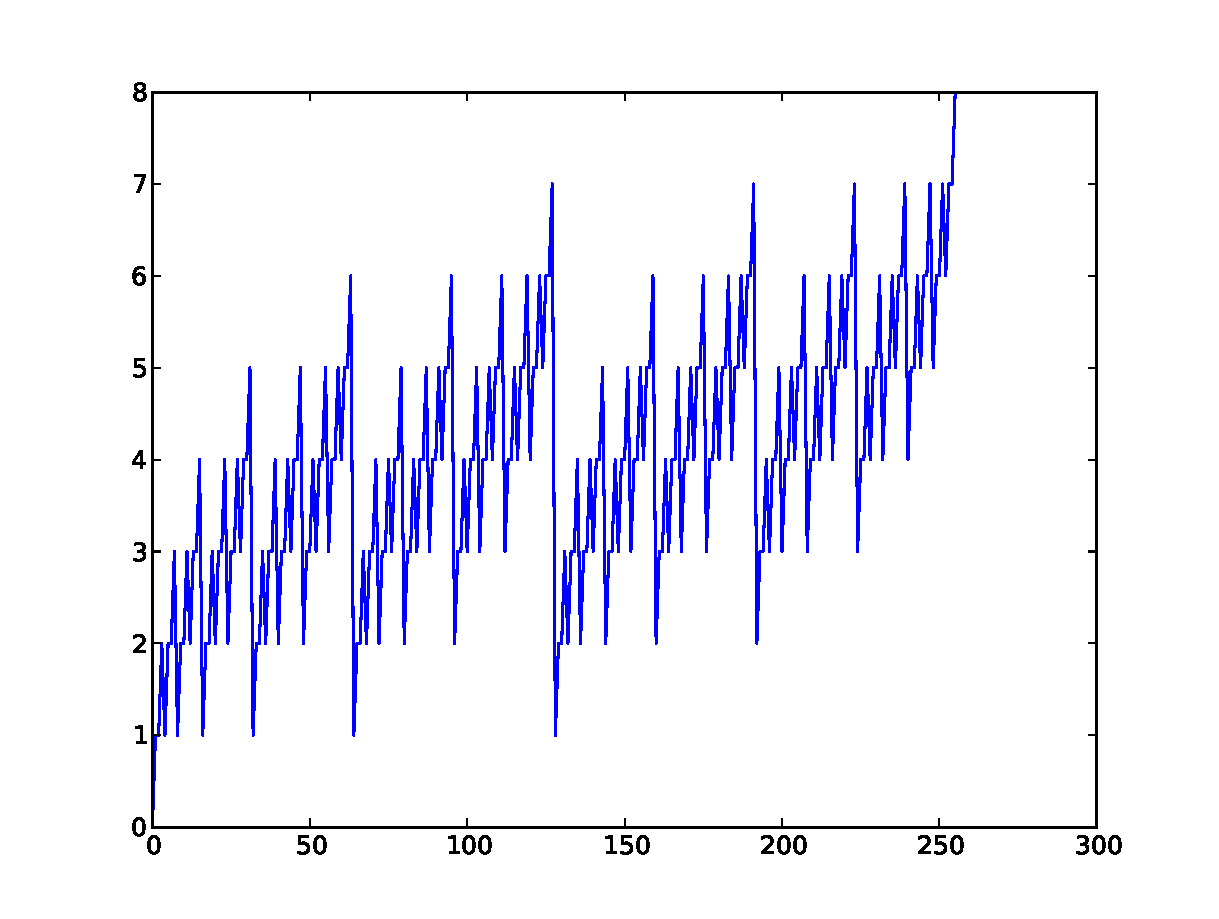
\includegraphics[width=3in]{part1.2/count-ones-plot.pdf}
    \caption{fitness function plot - count-ones\label{plot-count-ones}}
\end{figure} 

Figure~\ref{over-time-count-ones} shows how our optimization algorithms performed against the count ones function with an 80 bit input. Random hill climbing appeared to discover peaks quickly. However, the global optimum was not reached in many cases until twice the number of evaluations as simulated annealing. RHC also suffered from it's random restart behavior, which caused many function evaluations at much lower values of the function.

Simulated annealing was clearly the superior algorithm in this experiment. All 10 runs reached the global optimum within roughly 1,000 function evaluations, which represents 1/1\e{21} of the total input space. The genetic algorithm and MIMIC behaved well, making progress with each evaluation. However, they both required an order of magnitude greater evaluations to move toward the global optimum.

Given the relatively smooth trend of the function toward a global optimum, simulated annealing seems to have been able to explore the space well enough to move in that direction. As we will see later, finding a suitable temperature parameter is crucial for allowing the algorithm to move out of local optima. However, high temperatures keep the optimization task geared towards exploration longer than is necessary. In the case of this experiment, we happen to stumble on a good balance between exploration and exploitation.


\begin{figure}[!htbp]
    \centering
    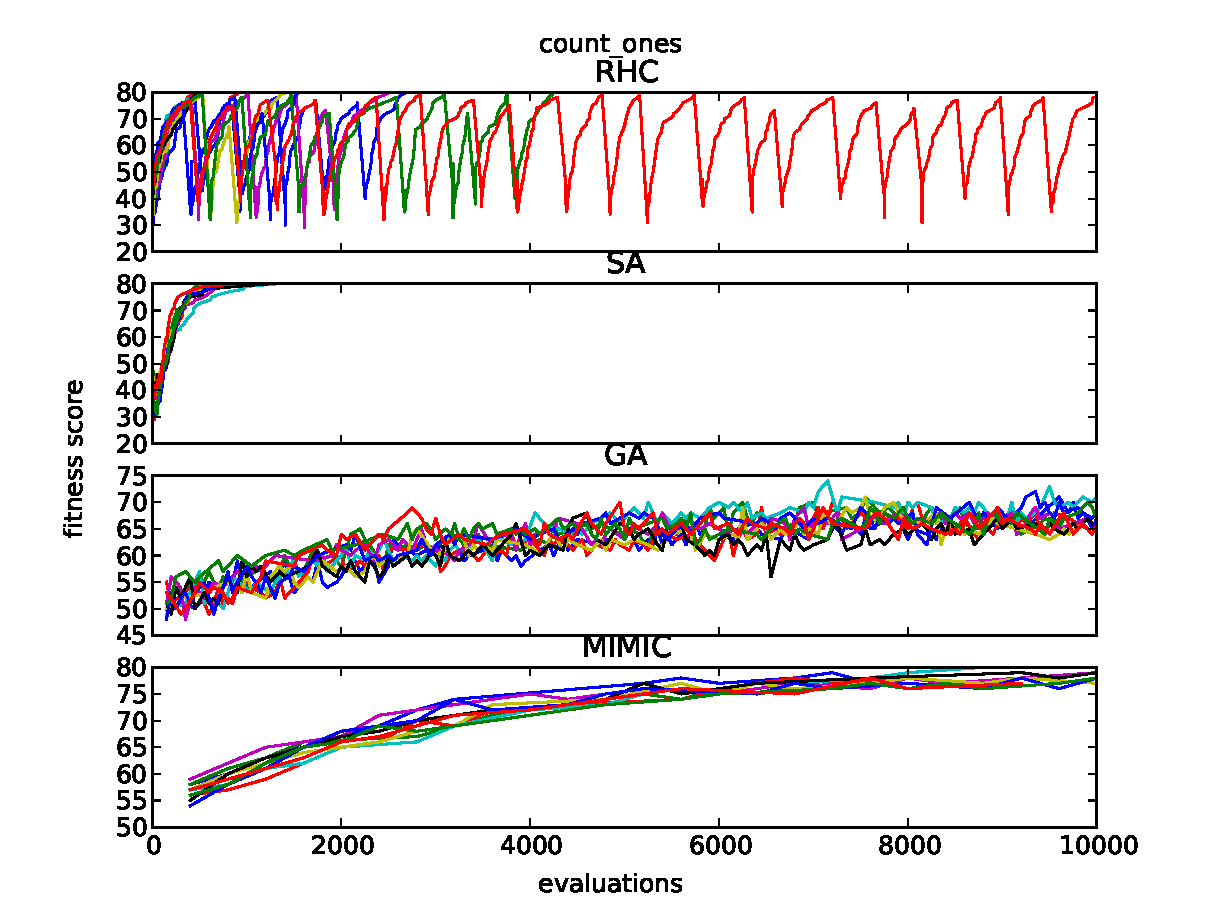
\includegraphics[width=3in]{part1.2/count-ones-over-time.pdf}
    \caption{fitness score by iteration - count-ones\label{over-time-count-ones}}
\end{figure} 

Each algorithm performed reasonably well at finding the global optimum for the count ones function at various input sizes, with the exception of our genetic algorithm. Given the somewhat unstructured and independent nature of the input bits, this is not surprising. MIMIC seemed to do well in this regard, despite the lack of structure. We could understand this to be a fortunate side effect of the probabilistic sampling, which causes the algorithm to perform similar to simulated annealing. Figure~\ref{max-count-ones} shows this behavior.

\begin{figure}[!htbp]
    \centering
    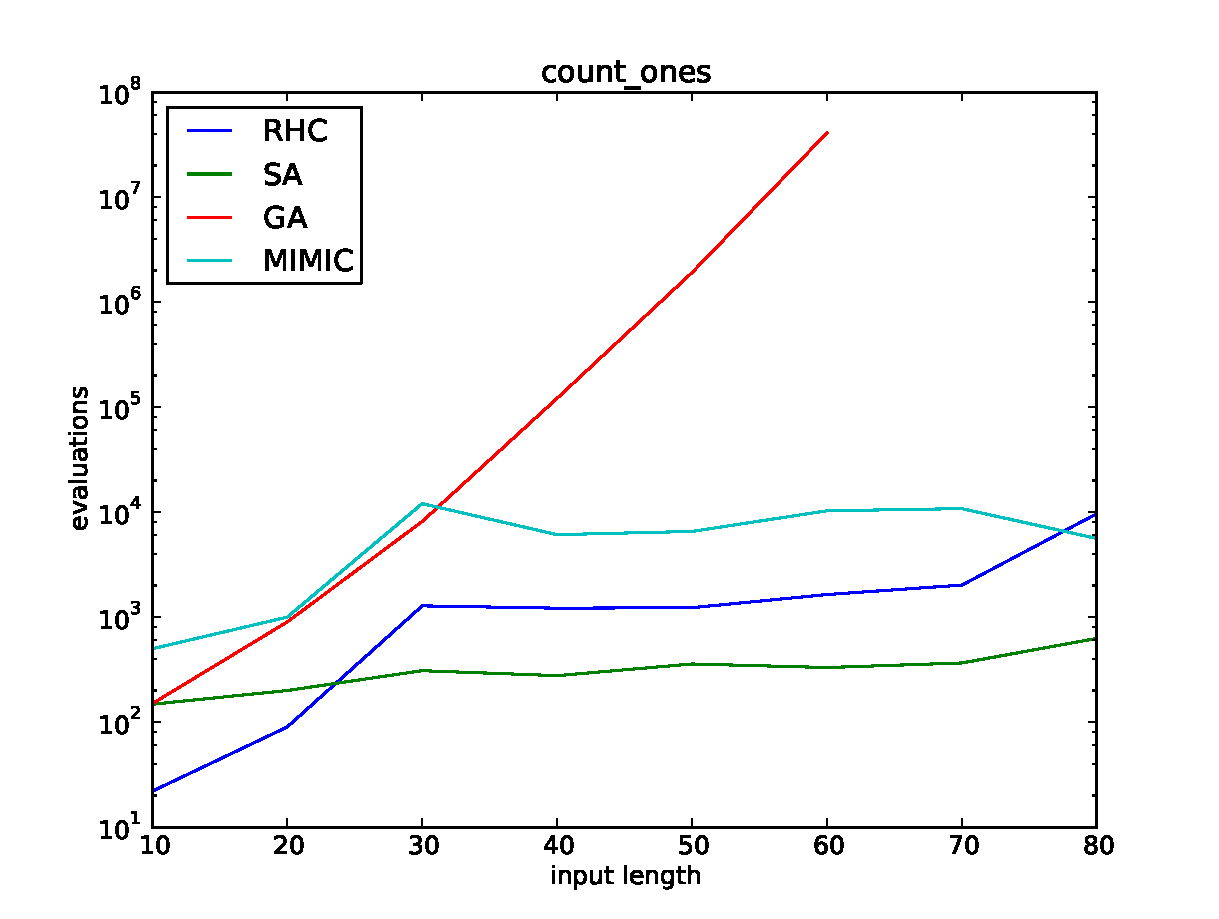
\includegraphics[width=3in]{part1.2/count-ones-max.pdf}
    \caption{iterations to find max - count-ones\label{max-count-ones}}
\end{figure} 


\subsubsection{Four Peaks}

The four peaks evaluation function is essentially a count of the leading 1s and trailing 0s in a bit string, with a bonus for having at least an arbitrary number of each. The plot of this function shows there are two global optima and a large number of local optima. There is also a point along the plot where values shift upwards. This is the point when the leading 1s reach the minimum number to get the bonus.

\begin{figure}[!htbp]
    \centering
    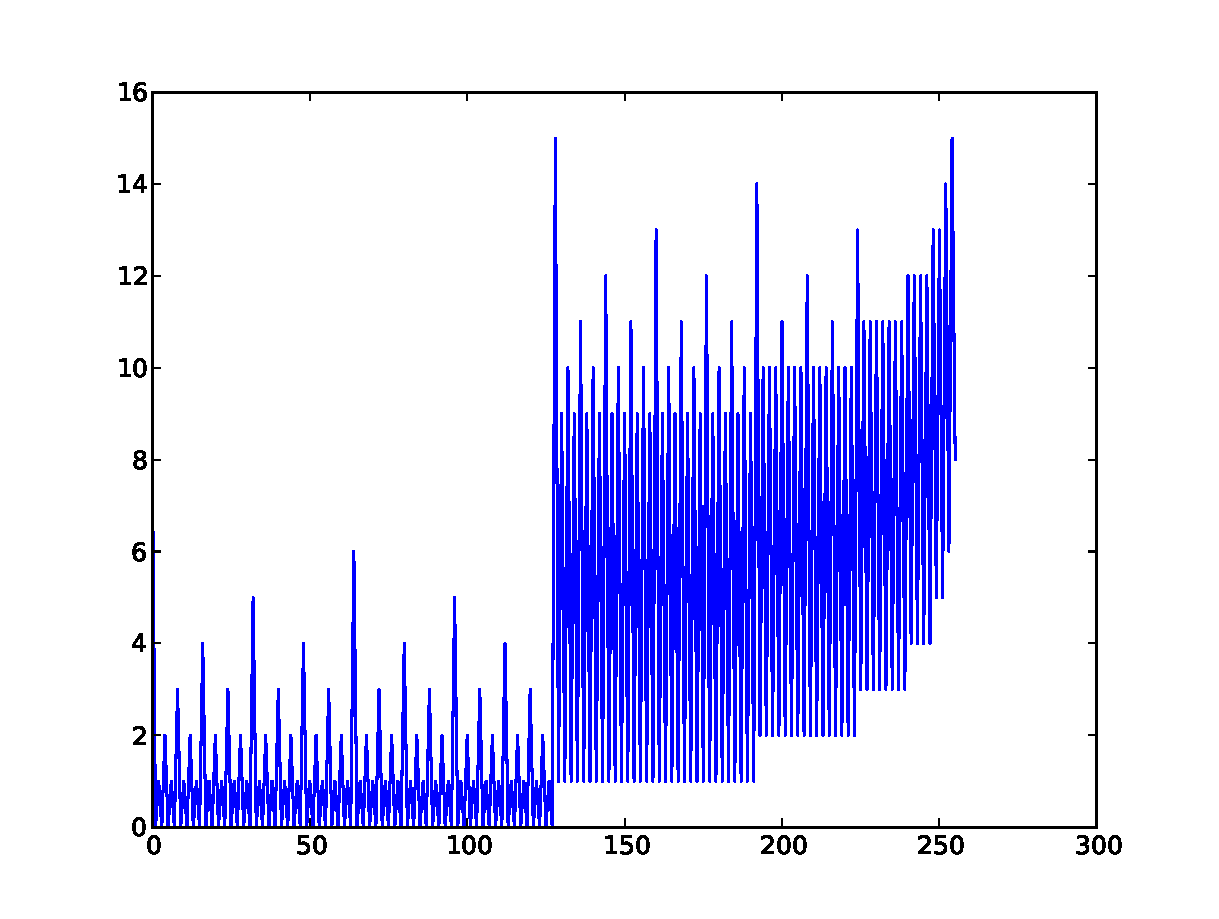
\includegraphics[width=3in]{part1.2/four-peaks-plot.pdf}
    \caption{fitness function plot - four-peaks\label{plot-four-peaks}}
\end{figure} 

Our genetic algorithm was able to find reasonably high valued input strings with a small number of function evaluations (Figure~\ref{over-time-four-peaks}. This makes sense given the structure of the input space and the fact that the algorithm would quickly evolve the population to include bit strings with better features (longer sets of leading 1s and trailing 0s). However, this algorithm did seem to struggle to find one of the two global optima.

This function also highlights the shortcomings of simulated annealing. Our plot shows that 7 out of 10 runs became permanently stuck in a local optimum. This is likely due to the sharp features of the landscape and insufficiently low temperature and overly rapid cooling rate. This caused the algorithm to get caught on a lower range of peaks.


\begin{figure}[!htbp]
    \centering
    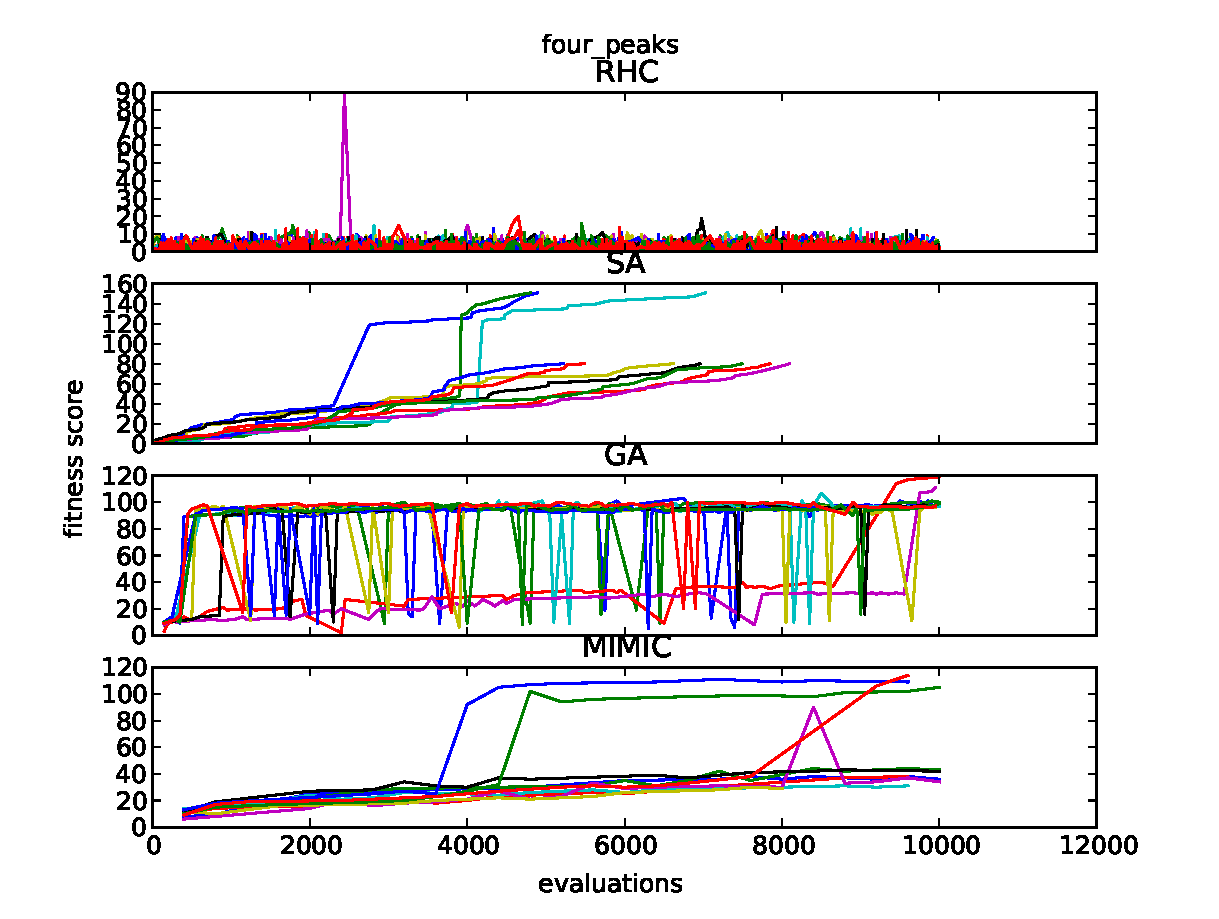
\includegraphics[width=3in]{part1.2/four-peaks-over-time.pdf}
    \caption{fitness score by iteration - four-peaks\label{over-time-four-peaks}}
\end{figure} 

Figure\ref{max-four-peaks} shows that although our genetic algorithm was able to quickly find input strings with high values, it required many more iterations to find the global optimum for a given input size. Conversely, despite the impressive figures for simulated annealing, we noted in the previous experiment how that algorithm was too likely to get caught in a local optimum. It required many more iterations of this experiment to get simulated annealing to find the global optimum at all.

MIMIC seemed to behave well in this case. Although it did not locate optimal values as quickly as the other algorithms, it showed steadily improving results over time and did not have the same difficulty with local optima. Also, in terms of iterations to finding the global optimum, MIMIC performed significantly better than the genetic algorithm for higher input sizes.

\begin{figure}[!htbp]
    \centering
    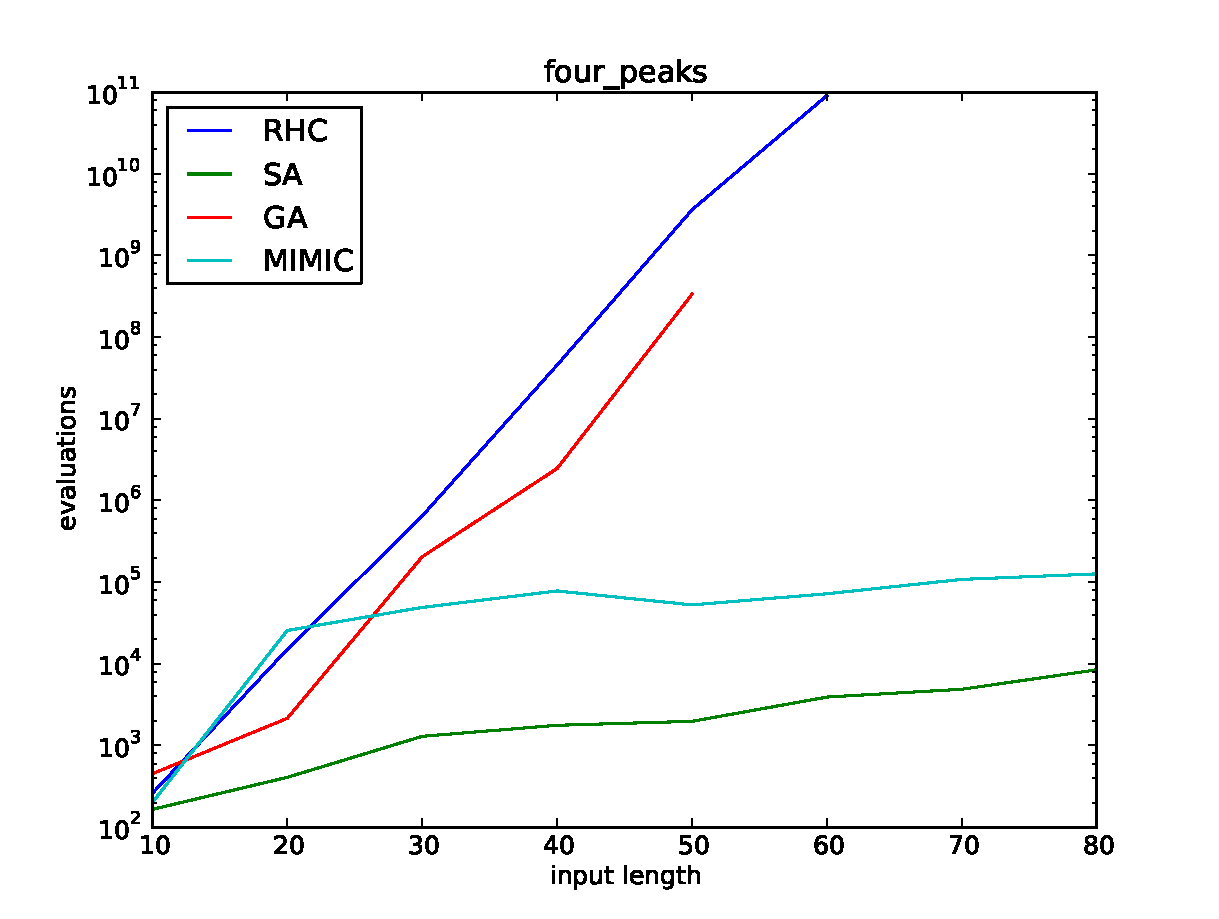
\includegraphics[width=3in]{part1.2/four-peaks-max.pdf}
    \caption{iterations to find max - four-peaks\label{max-four-peaks}}
\end{figure} 

\subsubsection{Flip Flop}

The flip flop fitness function is scored by adding one for each bit that has a different value than the next bit. There are two global optima for any given bit length and the function terrain is symmetrical over the input space, as we can see in Figure~\ref{plot-flip-flop}. This function combines features of both count ones and four peaks. It acts as a semi-structured function as each input bit has a relationship to the bit's on either side. However, there are two distinct optima with a completely opposite bit pattern.

\begin{figure}[!htbp]
    \centering
    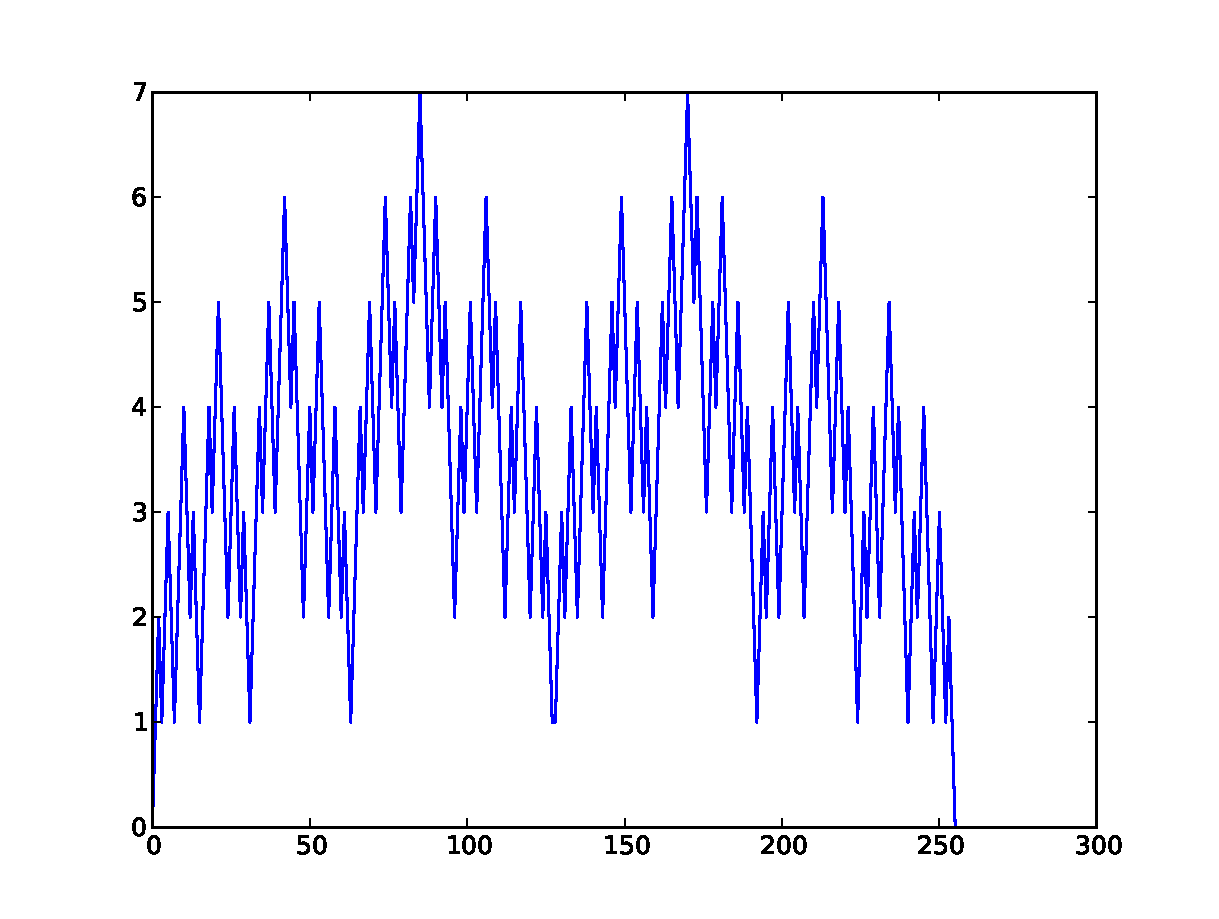
\includegraphics[width=3in]{part1.2/flip-flop-plot.pdf}
    \caption{fitness function plot - flip-flop\label{plot-flip-flop}}
\end{figure} 

Each of our three algorithms, not including random hill climbing, do well over time on this function. Simulated annealing is able to converge to high values of the function with significantly less evaluations than the other two. The genetic algorithm and MIMIC both move steadily toward higher values, but with many more evaluations. Mimic is able to do so with more consistent improvement and less variance in score along the way.

\begin{figure}[!htbp]
    \centering
    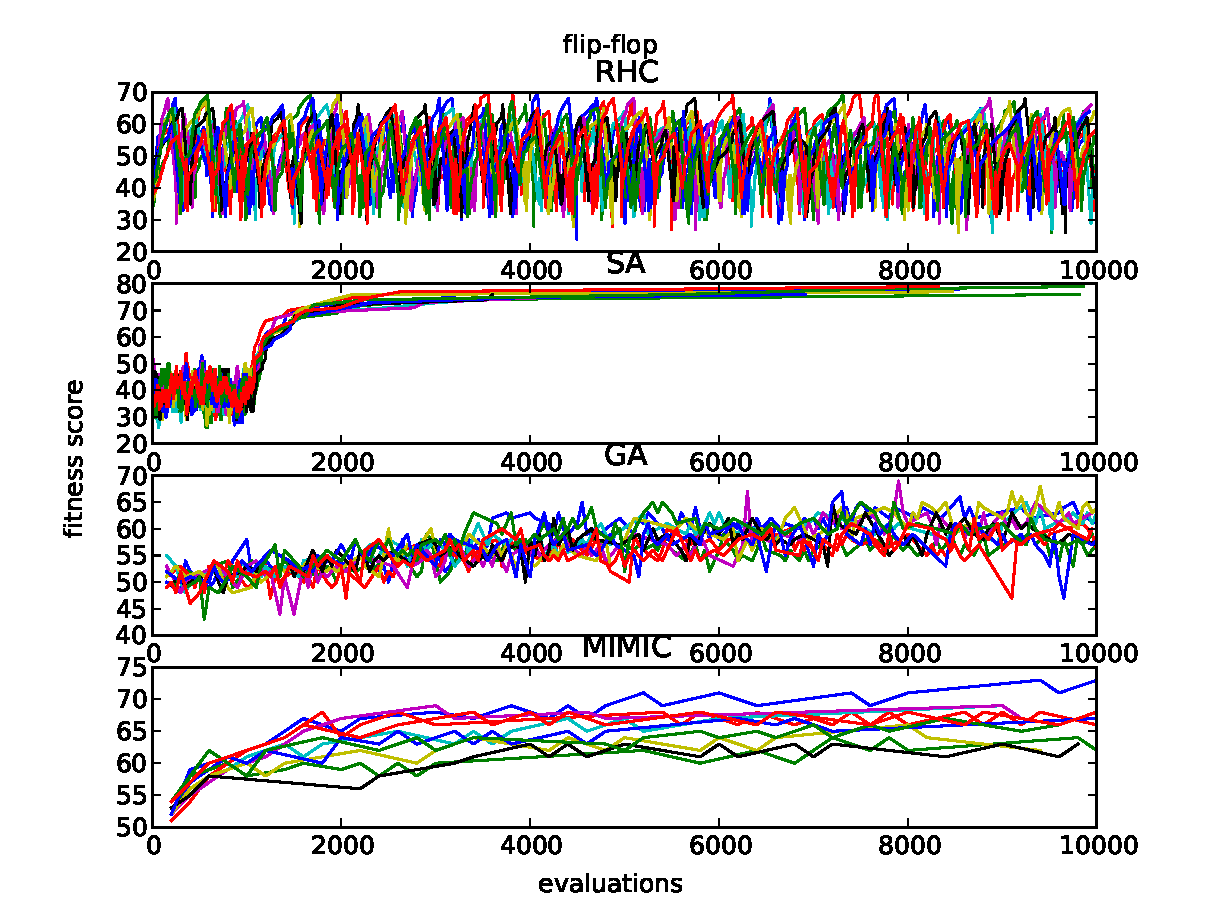
\includegraphics[width=3in]{part1.2/flip-flop-over-time.pdf}
    \caption{fitness score by iteration - flip-flop\label{over-time-flip-flop}}
\end{figure} 

Each algorithm was able to find the one of the optima within a closer number of evaluations than the previous fitness functions (Figure~\ref{max-flip-flop}. However, simulated annealing still performed orders of magnitude better than both MIMIC and the genetic algorithm in this experiment. 

\begin{figure}[!htbp]
    \centering
    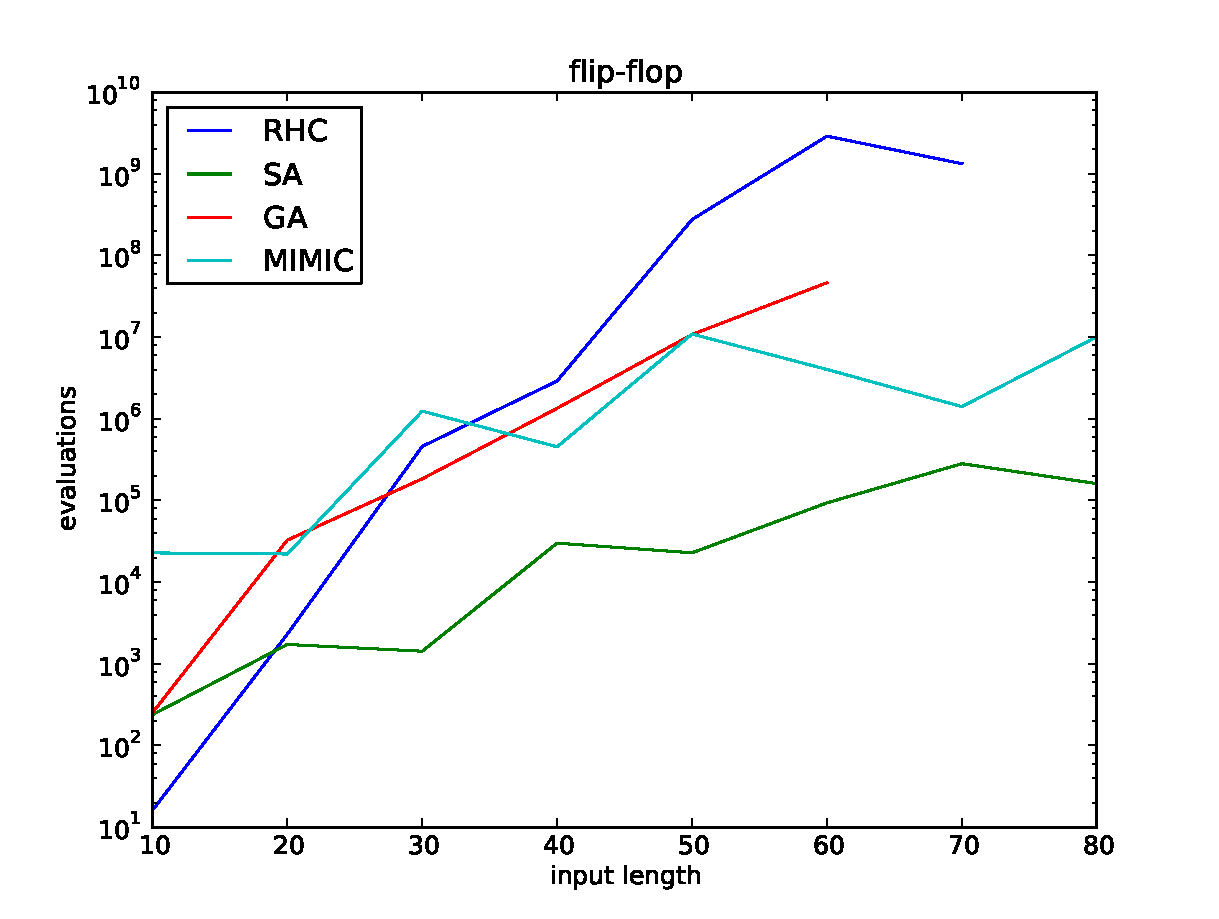
\includegraphics[width=3in]{part1.2/flip-flop-max.pdf}
    \caption{iterations to find max - flip-flop\label{max-flip-flop}}
\end{figure} 

%In addition to finding weights for a neural network, you must create three optimization problem domains on your own. For the purpose of this assignment an optimization problem is just a fitness function one is trying to maximize (as opposed to a cost function one is trying to minimize). This doesn't make things easier or harder, but picking one over the other makes things easier for us to grade.

%Please note that the problems you create should be over discrete-valued parameter spaces. Bit strings are preferable.

%The first problem should highlight advantages of your genetic algorithm, the second of simulated annealing, and the third of MIMIC. Be creative and thoughtful. It is not required that the problems be complicated or painful. They can be simple. For example, the 4-peaks and k-color problems are rather straightforward, but illustrate relative strengths rather neatly.


\section{Part 2: Unsupervised Learning Algorithms}

%You are to run a number of experiments. Come up with at least two datasets. If you'd like (and it makes a lot of sense in this case) you can use the ones you used in the first assignment or, if it makes any sense, the first part of this assignment.

\subsection{Exploring Dataset 1: Adult}

The first dataset we will explore is the same as from Part 1, the Adult dataset from UCI. To begin, we will first examine the distribution of instances by their class label. As we see in Figures~\ref{adult-attr-class}~and~\ref{adult-parallel-class}, groupings by class seem to occur based on attributes such as workclass, capital-gain, hour-per-week, and education. However, these groupings are not completely obvious and there are many non-conforming samples. As we will see with the results from our clustering task, the two class labels do not segment the data as well it could be done.

\begin{figure}[!htbp]
    \centering
    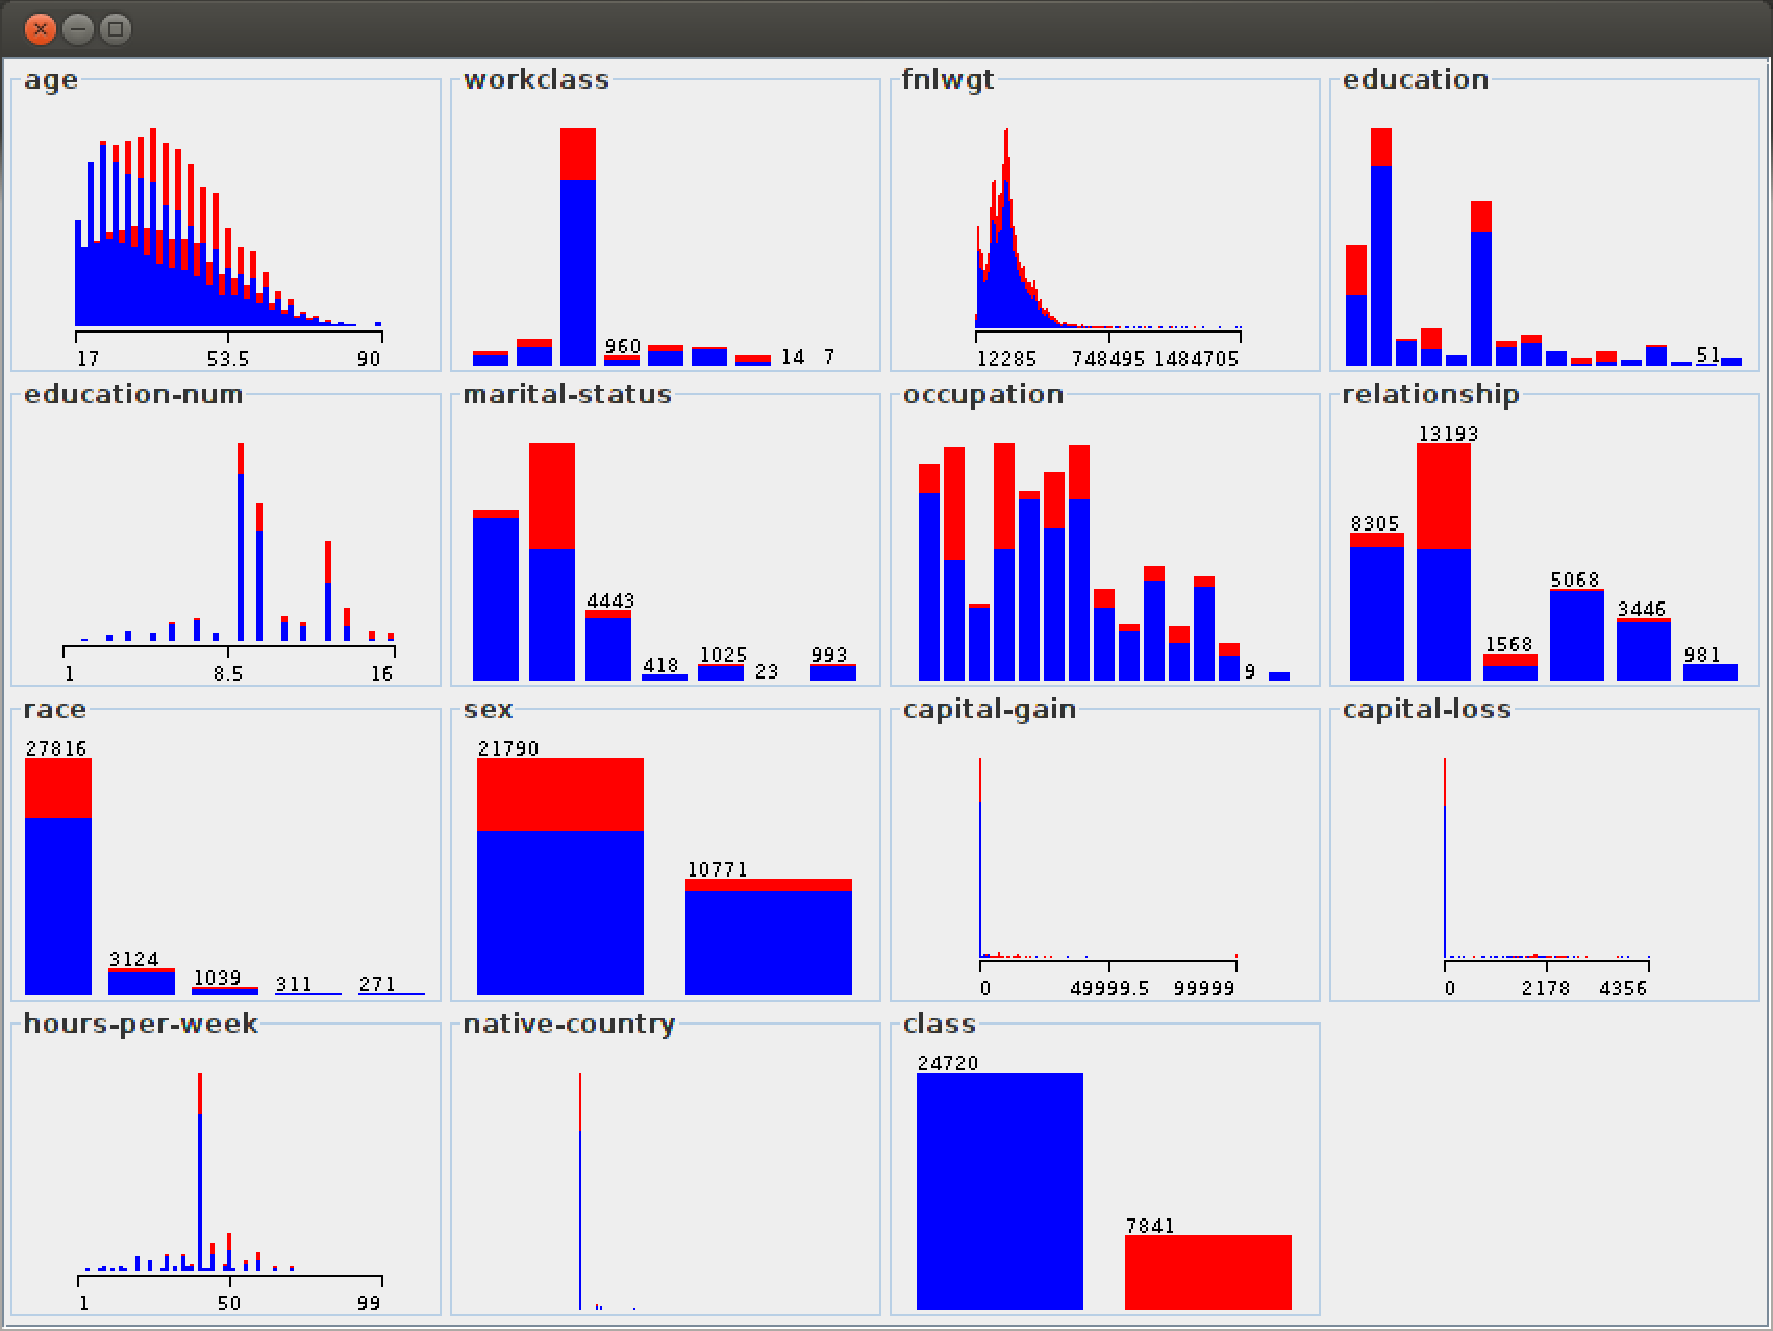
\includegraphics[width=3in]{part2/adult/attr-class.pdf}
    \caption{dataset attributes - adult\label{adult-attr-class}}
\end{figure} 

\begin{figure}[!htbp]
    \centering
    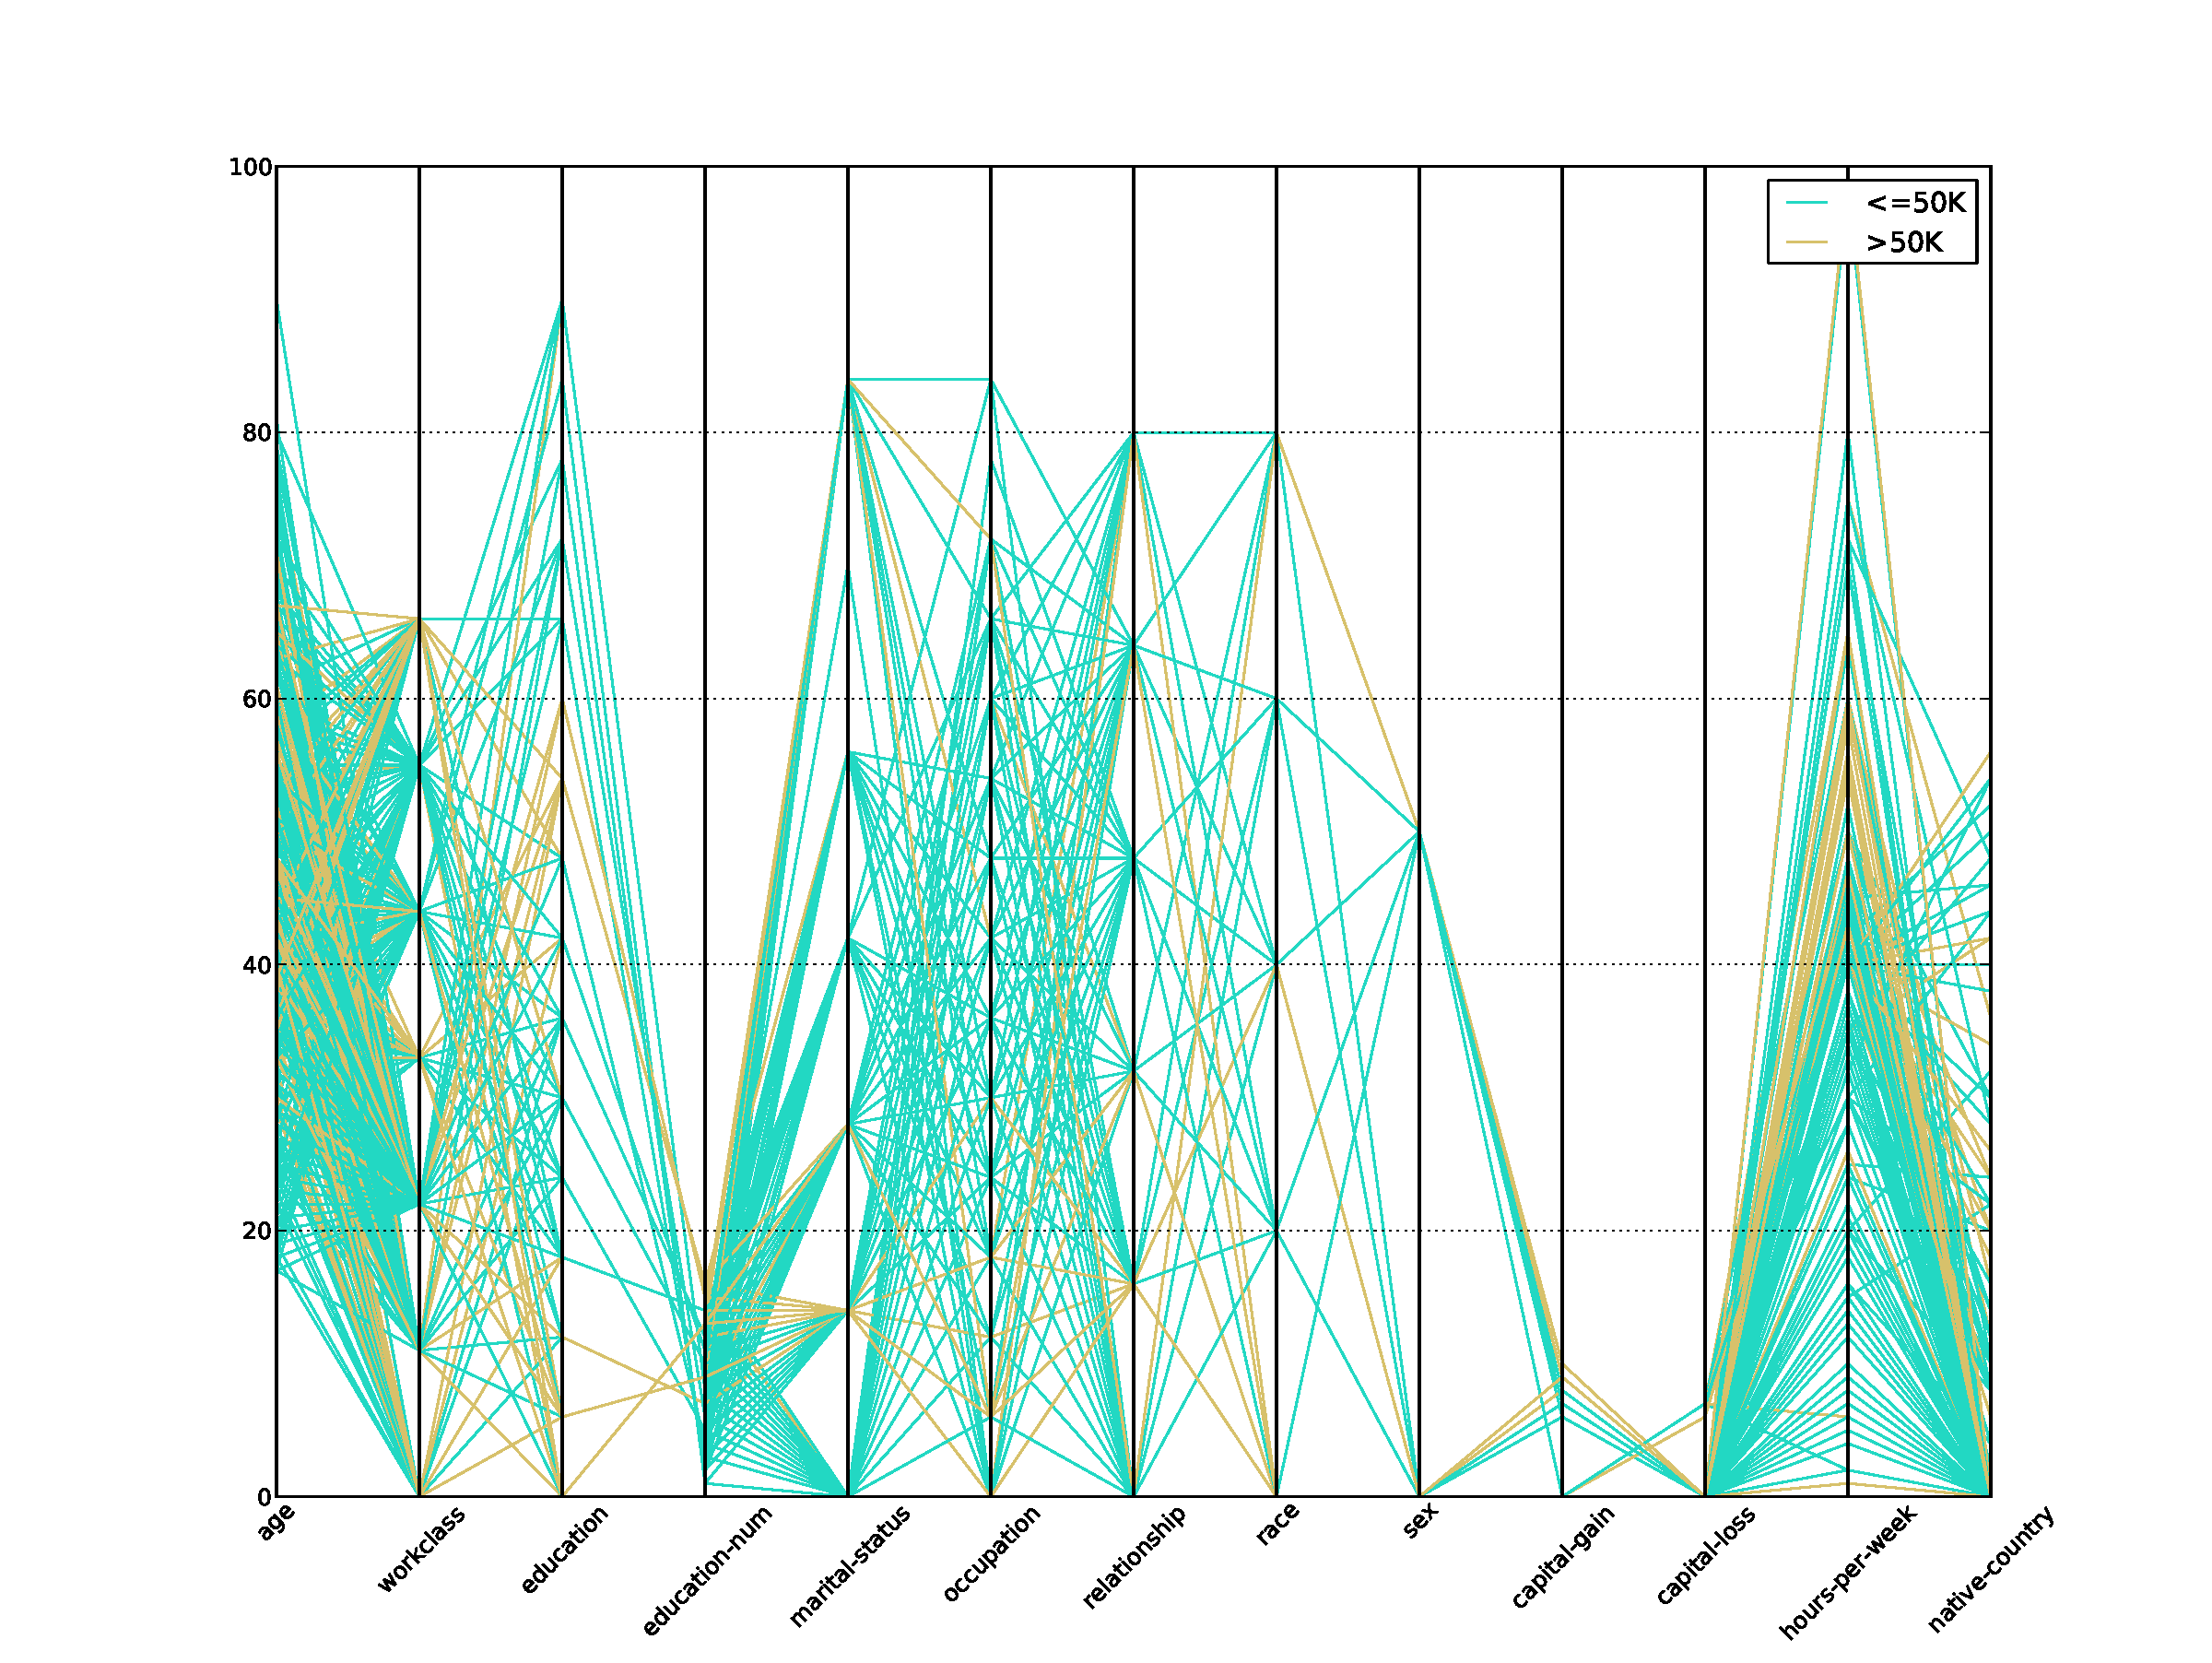
\includegraphics[width=3in]{part2/adult/parallel-class.pdf}
    \caption{dataset parallel plot - adult\label{adult-parallel-class}}
\end{figure} 

\subsubsection{Clustering}

%Run the clustering algorithms on the data sets and describe what you see.

In order to determine the optimal value for K, we can iterate through increasing values and compare a metric that gives an idea of how well our data is segmented into each cluster. In this first case, the expectation maximization algorithm was run with increasing values of K, and the resulting log likelihood value was compared. This is a default option in the Weka implementation of the algorithm. Larger and smaller values of K were run to validate the result through visual inspection of the resulting cluster features. For the Adult dataset, a cluster size of three resulted in the greatest log likelihood, and the clusters made sense when viewing the resulting cluster attributes.

Form the results of k-means (Figure~\ref{kmeans-summary}) and EM (Figure~\ref{kmeans-summary}) clustering, three distinct profiles emerge from the data:

\paragraph{Cluster 1 - Young and poor}
\begin{itemize}[itemsep=1pt]
    \item Young (34)
    \item Less educated (9.8)
    \item Single (Never-married, Divorced, Separated, Widowed)
    \item Works less hours (37.5)
    \item Low income (<50k)
\end{itemize}

\paragraph{Cluster 2 - Older and experienced}
\begin{itemize}[itemsep=1pt]
    \item Older (43)
    \item More educated (12.5)
    \item Male
    \item High cap gain/loss (5000/475)
    \item Works more hours (44.8)
    \item High income (>50k)
\end{itemize}

\paragraph{Cluster 3 - Older blue collar}
\begin{itemize}[itemsep=1pt]
    \item Older (43)
    \item less educated (9.8)
    \item Currently Married
    \item Male
    \item Works medium hours (43)
    \item Low income (<50k)
\end{itemize}



\tiny
\begin{verbbox}
Running k-means

Within cluster sum of squared errors: 94691.74506148841
Missing values globally replaced with mean/mode

Cluster centroids:
                                     Cluster#
Attribute           Full Data               0              1              2
                      (32561)          (7243)        (14601)        (10717)
===========================================================================
age                   38.5816         43.6339        32.9471        42.8437
workclass             Private         Private        Private        Private
fnlwgt            189778.3665     187061.4272    192070.6165    188491.5931
education             HS-grad       Bachelors        HS-grad        HS-grad
education-num         10.0807         12.6281         9.8104         8.7273
marital-status        Married         Married  Never-married        Married
occupation     Prof-specialty  Prof-specialty   Adm-clerical   Craft-repair
relationship          Husband         Husband  Not-in-family        Husband
race                    White           White          White          White
sex                      Male            Male         Female           Male
capital-gain        1077.6488       3607.9214       269.1136       469.1444
capital-loss          87.3038        179.5659        50.7723        74.7204
hours-per-week        40.4375         45.0614        36.5254        42.6422
native-country  United-States   United-States  United-States  United-States
class                   <=50K            >50K          <=50K          <=50K
\end{verbbox}
\normalsize

\begin{figure}[!htbp]
    \centering
    \theverbbox
    \caption{k-means clustering results\label{kmeans-summary}}
\end{figure}


\scriptsize
\begin{verbbox}
EM
==

Number of clusters selected by cross validation: 3


                     Cluster
Attribute                  0           1           2
                      (0.53)      (0.18)      (0.28)
=====================================================
age
  mean                34.4071     43.6058     43.2169
  std. dev.           13.4275     11.5698     12.6479

education-num
  mean                 9.8028     12.4534        9.07
  std. dev.            2.3915      2.2579      2.1192

relationship
   Not-in-family    7417.5347    732.4946    157.9707
   Husband             6.5078    4459.228   8730.2642
   Wife             1044.7802     372.591    153.6288
   Own-child         4842.923     166.438      61.639
   Unmarried        3189.2812    193.3051     66.4137
   Other-relative    899.9176     41.2378     42.8447
  [total]          17400.9445   5965.2944   9212.7611
sex
   Male             7798.0266   5069.9658   8925.0076
   Female           9598.9179    891.3286    283.7535
  [total]          17396.9445   5961.2944   9208.7611
capital-gain
  mean                  4.065   5506.3843     239.438
  std. dev.           60.7467  16515.2342    873.4603

capital-loss
  mean                      0    475.4836      0.9942
  std. dev.          402.9602    837.7166     25.1187

hours-per-week
  mean                37.5504     44.8544     43.0332
  std. dev.           12.1264     11.7279     11.7133

class
   <=50K           16342.7922   1688.2196   6691.9882
   >50K             1054.1523   4273.0749   2516.7729
  [total]          17396.9445   5961.2944   9208.7611


Time taken to build model (full training data) : 395.06 seconds

=== Model and evaluation on training set ===

Clustered Instances

0      17815 ( 55%)
1       4160 ( 13%)
2      10586 ( 33%)

Log likelihood: -46.47694
\end{verbbox}
\normalsize

\begin{figure}[!htbp]
    \centering
    \theverbbox
    \caption{subset of EM clustering results\label{em-summary}}
\end{figure}

Visualizing the samples based on their cluster assignments shows a somewhat clearer distinction than their class assignment plots. Figures~\ref{adult-attr-cluster}~and~\ref{adult-parallel-cluster} show these distributions. Figure~\ref{adult-parallel-cluster} provides a better picture of the groupings. We can see in this visualization how younger individuals cluster in their marital-status, relationship, capital gains, hours-per-week, and income class. Likewise, we see the profile pattern for the older, experienced, group (yellow). These individuals share the attributes of being older, having higher education levels, higher capital-gains, and more hours-per-week. It should be noted that although these grouping are clear enough to see upon examination, they do not stand out with complete distinctiveness. There is a significant amount of noise in the data, which many samples that do not conform the to complete set of common profile attributes.

\begin{figure}[!htbp]
    \centering
    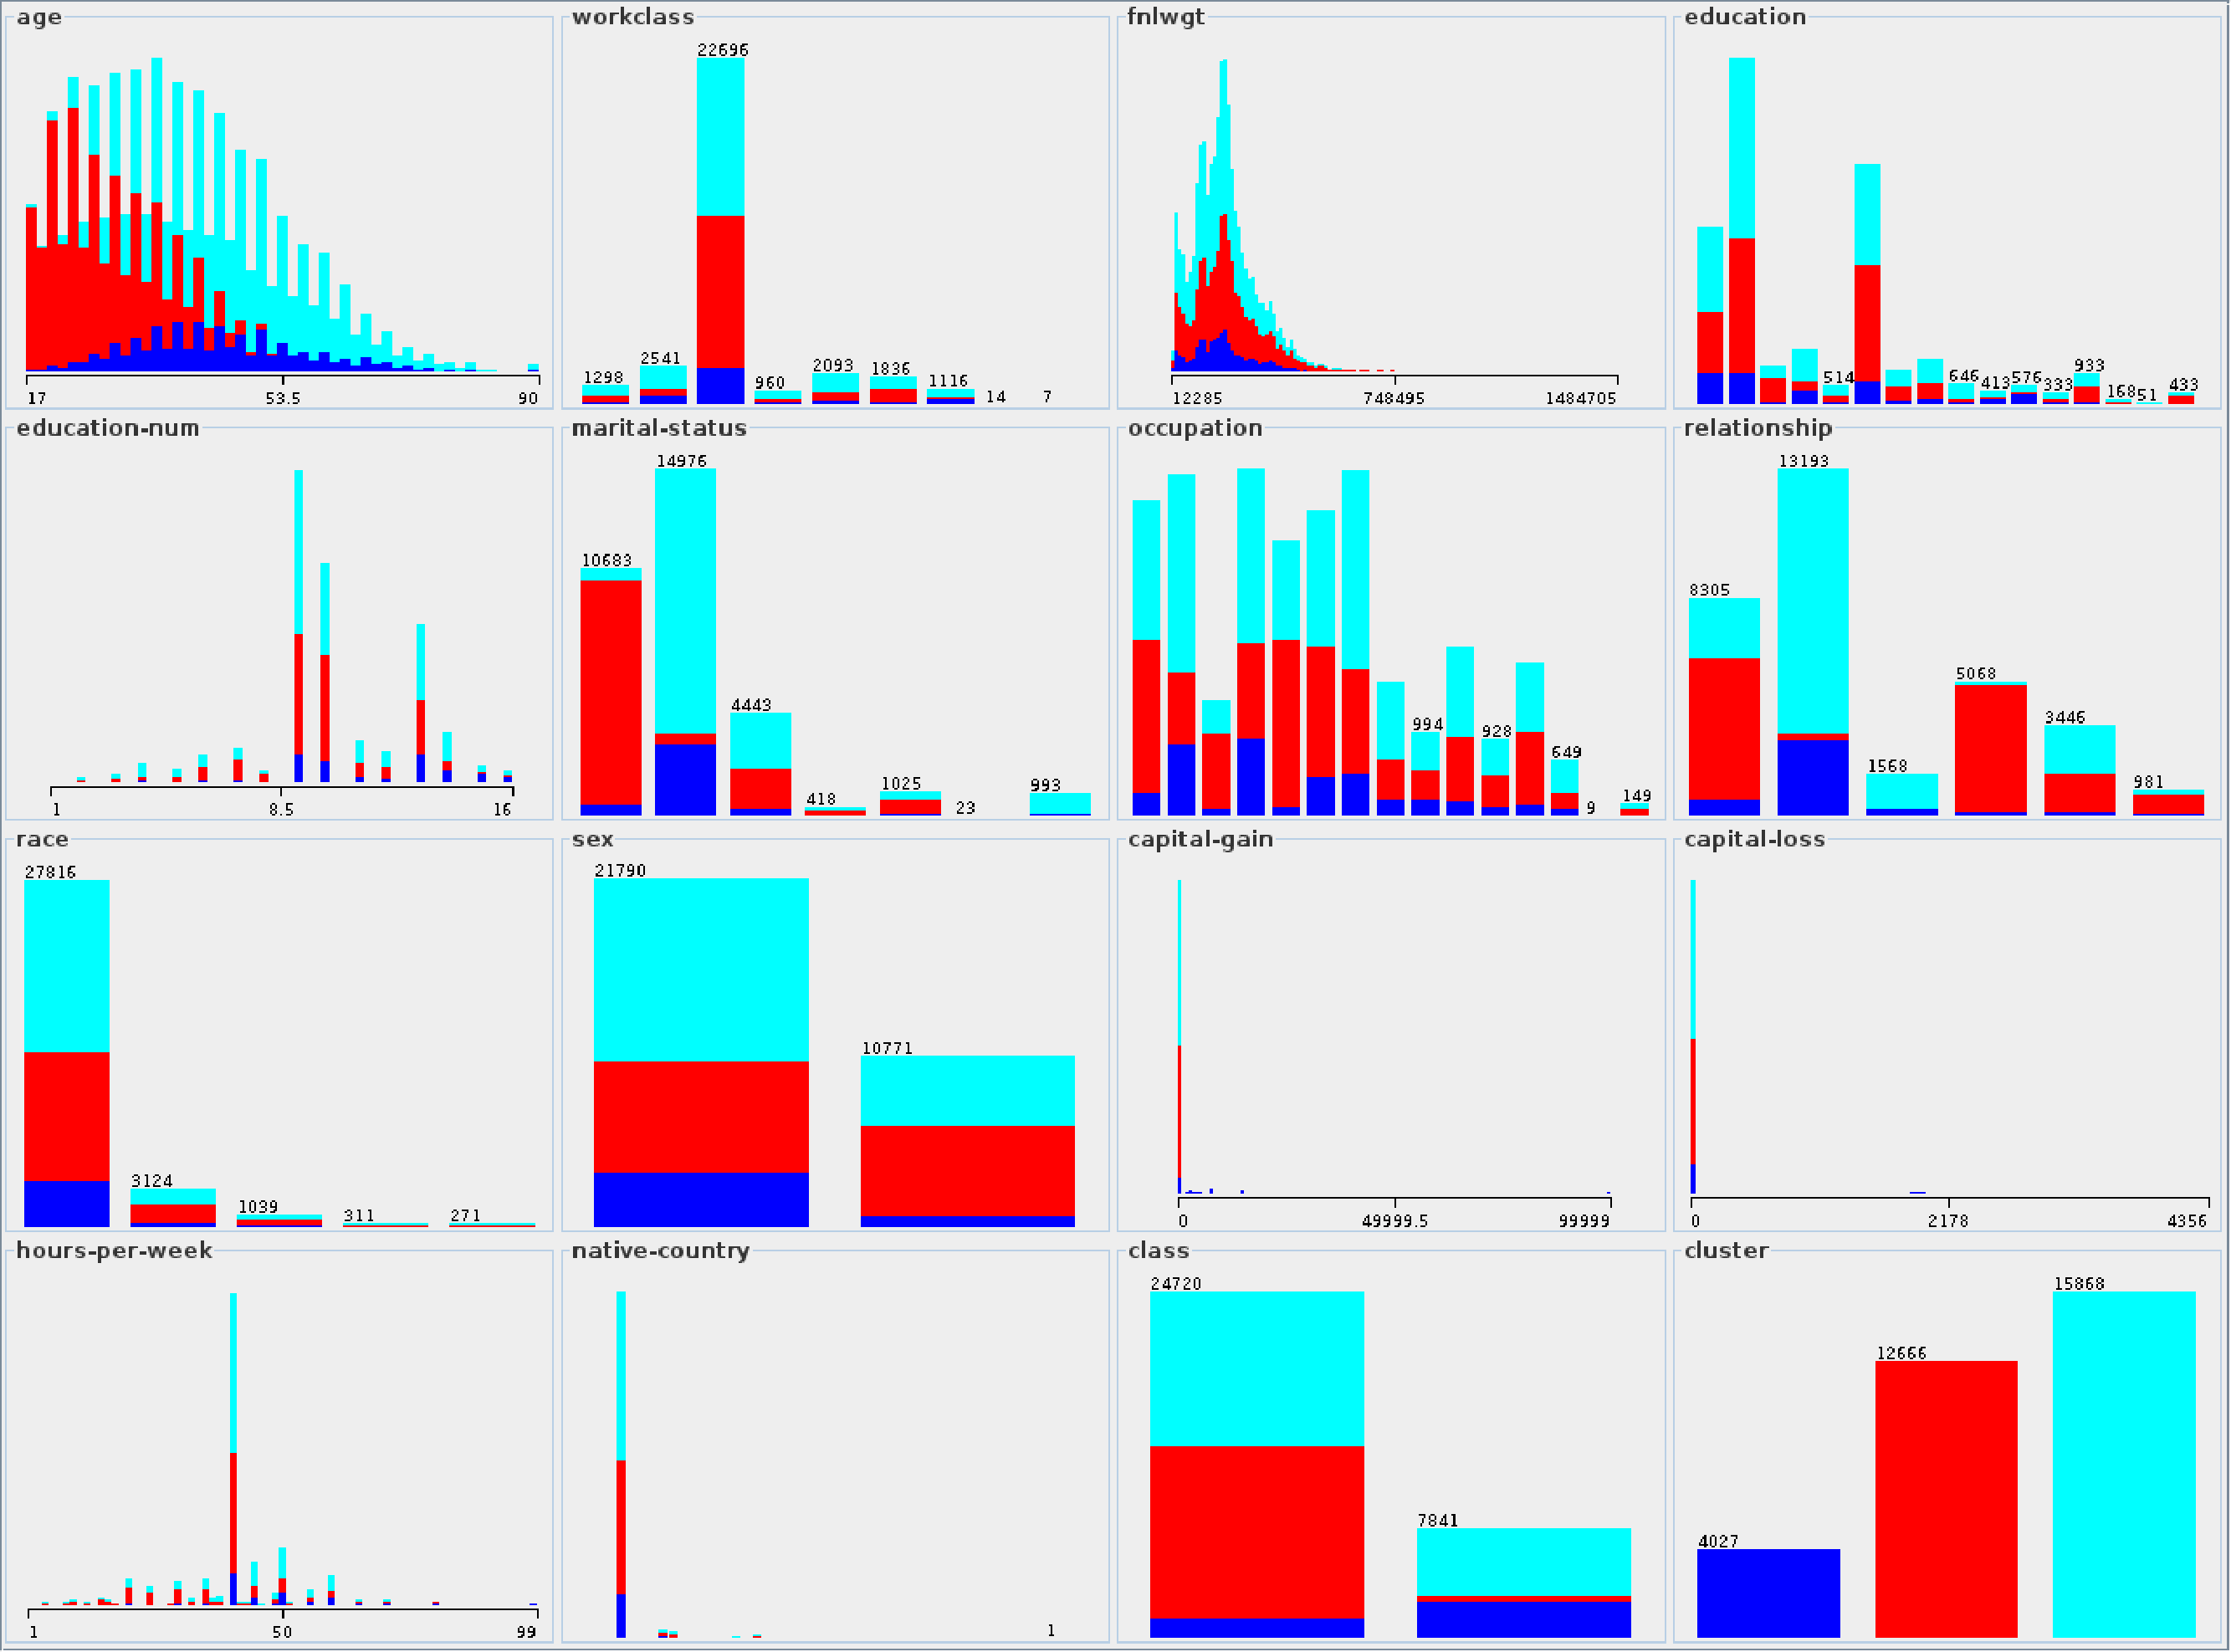
\includegraphics[width=3in]{part2/adult/attr-cluster.pdf}
    \caption{dataset attributes by cluster - adult\label{adult-attr-cluster}}
\end{figure} 

\begin{figure}[!htbp]
    \centering
    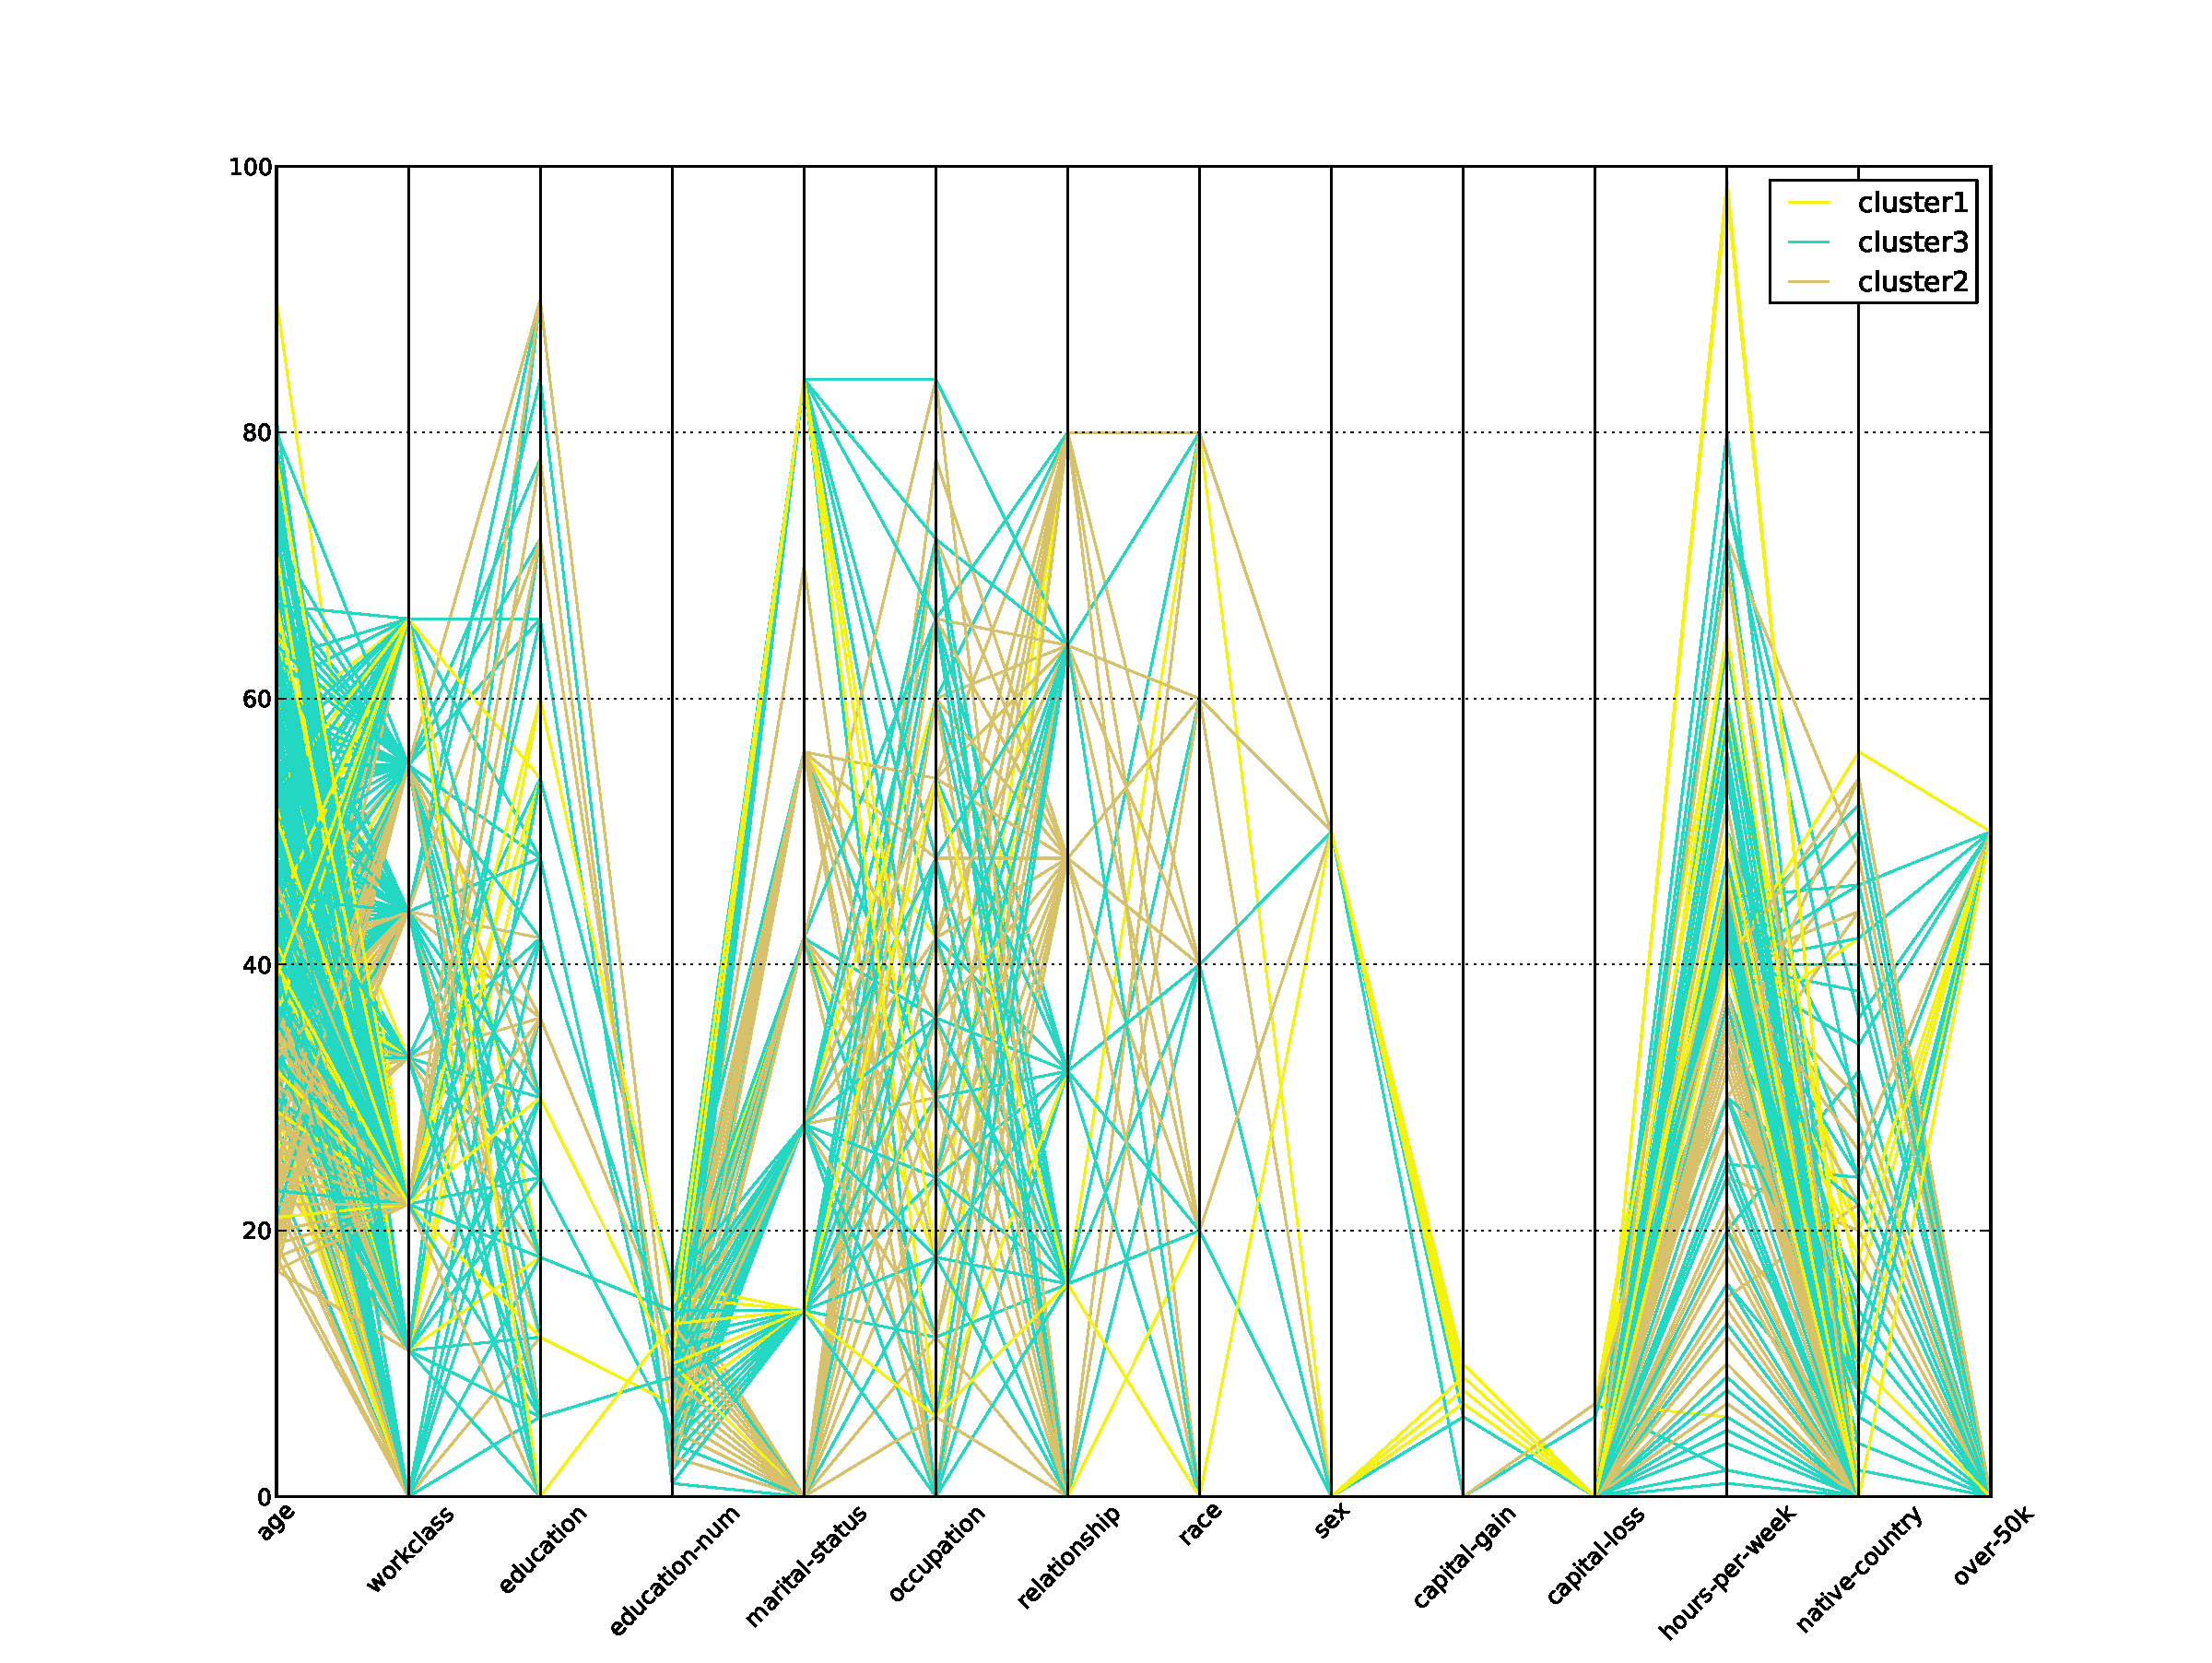
\includegraphics[width=3in]{part2/adult/parallel-cluster.pdf}
    \caption{dataset parallel plot by cluster - adult\label{adult-parallel-cluster}}
\end{figure} 


\subsubsection{Clustering on Dimensionally Reduced Dataset}

%Apply the dimensionality reduction algorithms to the two datasets and describe what you see.

\paragraph{PCA}
Running PCA on the Adult dataset results in features with the characteristics shown in Figure~\ref{pca-adult}. The first few principle components capture 11\% of the dataset variance. The distribution of eigenvalues shows that the roughly the first five components distinguish themselves in regards to their contribution to the overall variance.


\begin{verbbox}
eigenvalue  proportion  cumulative
4.13178     0.03861     0.03861
2.89985     0.0271      0.06572
2.5952      0.02425     0.08997
2.42699     0.02268     0.11265
2.23305     0.02087     0.13352
1.90511     0.0178      0.15133
1.63445     0.01528     0.1666 
1.5871      0.01483     0.18143
1.49286     0.01395     0.19539
1.42284     0.0133      0.20868
1.37072     0.01281     0.22149
1.31255     0.01227     0.23376
1.29281     0.01208     0.24584
1.2507      0.01169     0.25753
1.23304     0.01152     0.26906
1.21991     0.0114      0.28046
1.19888     0.0112      0.29166
1.17351     0.01097     0.30263
1.16087     0.01085     0.31348
1.14374     0.01069     0.32417
1.12887     0.01055     0.33472
1.12004     0.01047     0.34519
1.11544     0.01042     0.35561
1.09716     0.01025     0.36586
1.09448     0.01023     0.37609
1.08928     0.01018     0.38627
1.08335     0.01012     0.3964 
1.07809     0.01008     0.40647
1.06987     0.01        0.41647
\end{verbbox}

\begin{figure}[!htbp]
    \centering
    \theverbbox
    \caption{PCA eigenvalues - adult\label{pca-adult}}
\end{figure}

Clustering on the first five components from our resulting PCA features creates clusters with much clearer distinctions than with the original 14 attributes. Figure~\ref{pca-cluster-scatter} shows the cluster assignments based on only the first component (spread out over the instance numbers). With just this single attribute, we can see a clearer segregation of our three clusters. Log likelihood from EM clustering came out to -9.15, which is significantly higher than -46.5 achieved with the original attributes. K-means clustering resulted in a similar plot, and a sum of squared errors within each cluster of 2,620.

\begin{figure}[!htbp]
    \centering
    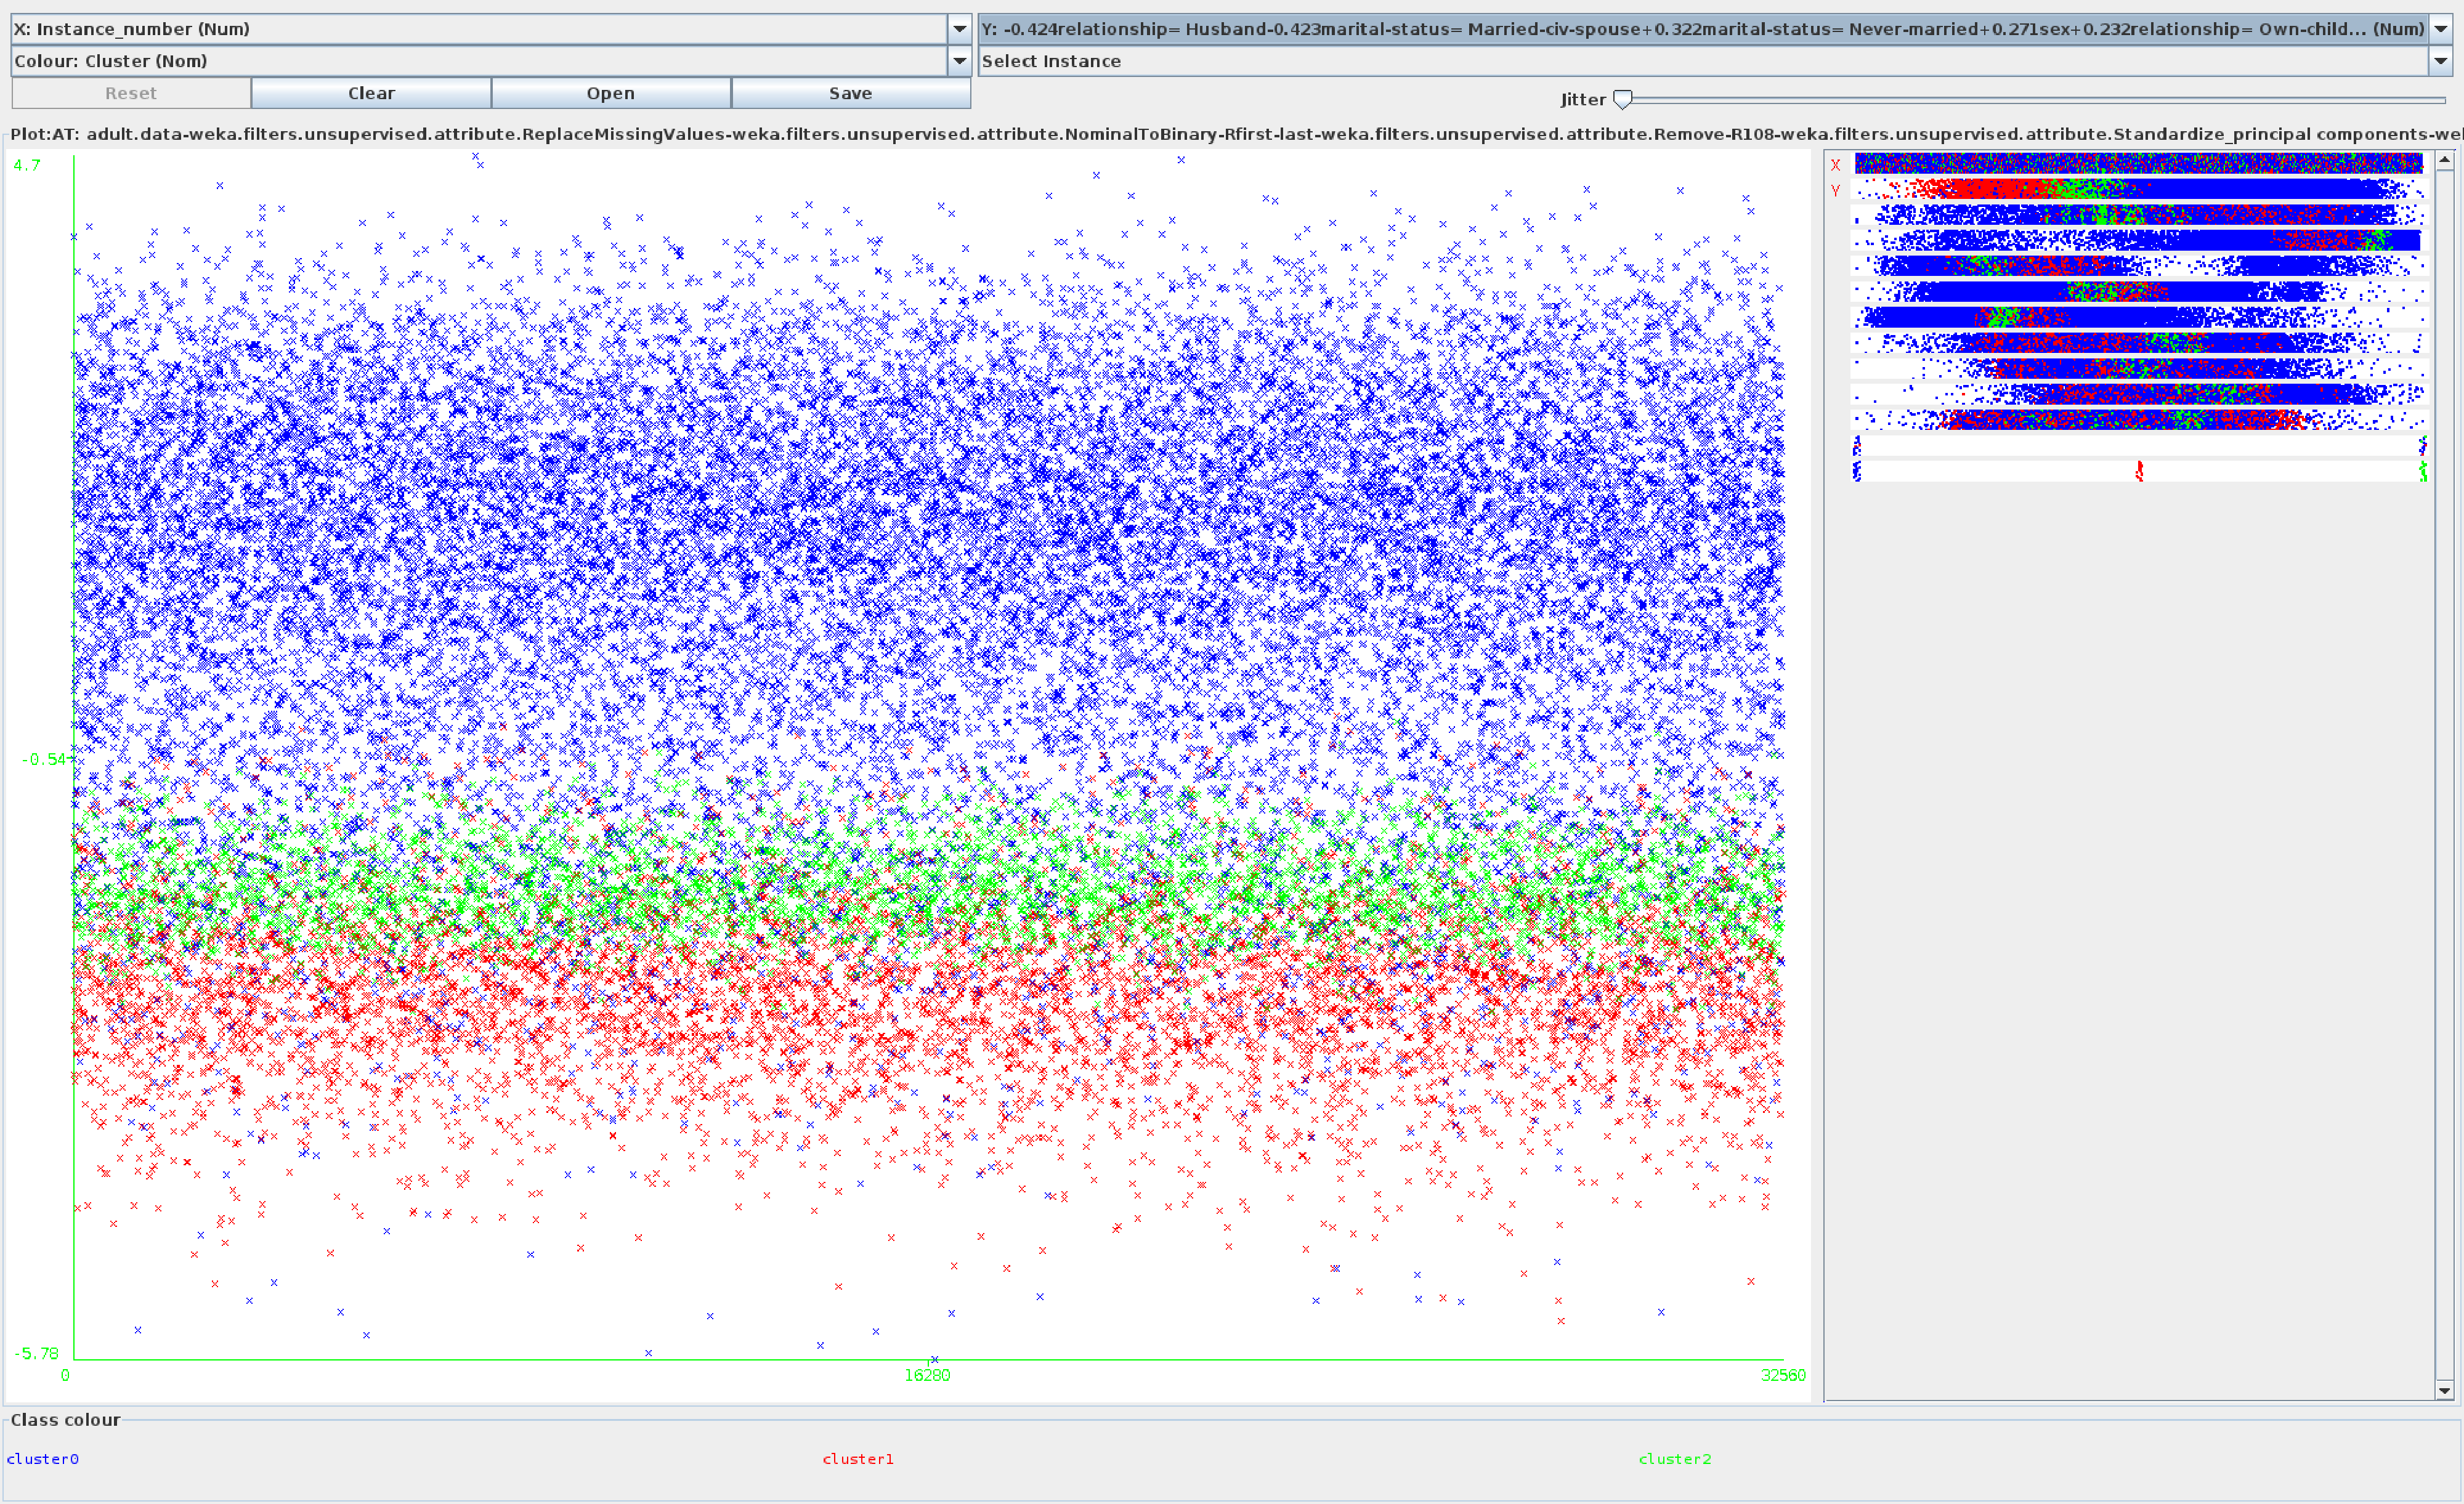
\includegraphics[width=3in]{part2/adult/pca-cluster-scatter.pdf}
    \caption{pca clusters on fist component - adult\label{pca-cluster-scatter}}
\end{figure} 


\paragraph{ICA}

Running independent component analysis on the dataset required a decision regarding the number of independent features to output. Without foreknowledge, experimentation was necessary to find an appropriate number of components. This was accomplished by iterating up to the original number of features, running ICA with that number of target components, and comparing the resulting kurtosis to determine how well ICA was able to pull independent features from the mixed uniform distribution. The intuition begin that a set of features with a high absolute biased kurtosis (zeroed at normal distribution), would indicate significant, independent, contributing features.

The result of this experiments can be seen in Figure~\ref{ica-stats-adult}. From this data we can make an informed decision regarding how many components to output from ICA for use in our clustering task. 

\tiny
\begin{verbbox}
  n  min/max                  mean            var         skew    kurtosis
---  ------------------  ---------  -------------  -----------  ----------
  1  (6.217, 6.21775)     6.21775      0           0             -3
  2  (35.31, 45.3218)    40.3204      50.0296      2.15814e-15   -2
  3  (6.214, 154.845)    60.4781    6729.09        0.683477      -1.5
  4  (0.2694, 155.271)   45.5331    5423.68        1.11028       -0.703042
  5  (0.2143, 155.314)   37.0787    4428.31        1.45134        0.180383
  6  (1.399, 155.273)    35.3957    3554.86        1.67272        0.985259
  7  (0.222, 155.400)    30.6465    3132.59        1.90229        1.84921
  8  (0.0771, 155.355)   26.9649    2793.2         2.11254        2.72931
  9  (0.2083, 155.775)   24.3725    2519.2         2.31297        3.63809
 10  (0.3312, 155.651)   22.0006    2291.2         2.49168        4.53032
 11  (0.4255, 155.747)   20.3085    2095.81        2.66496        5.44675
 12  (0.1315, 155.606)   19.2382    1914.82        2.8292         6.37344
 13  (0.1338, 155.619)   20.6722    1781.69        2.78072        6.45888
 14  (0.6387, 0.817448)   0.721304     0.00240131  0.167194      -0.364713
\end{verbbox}
\normalsize

\begin{figure}[!htbp]
    \centering
    \theverbbox
    \caption{ICA kurtosis stats by number of features - adult\label{ica-stats-adult}}
\end{figure}

Reducing to three components resulted in kurtosis of [6.2, 154.8, 20.3]. This signifies three, non-normally distributed, independent features. Performing EM and k-means clustering on the ICA filtered dataset resulted in a tight clusters (EM log likelihood: 23.5, k-means SSE: 270.4). Visualization of these clusters is shown in Figure~\ref{parallel-ica-cluster}. These show much more distinct groupings than with the original data. The EM clustering task took 12 seconds with these features, which is nearly half the time it required to process the original 14 features.

\begin{figure}[!htbp]
    \centering
    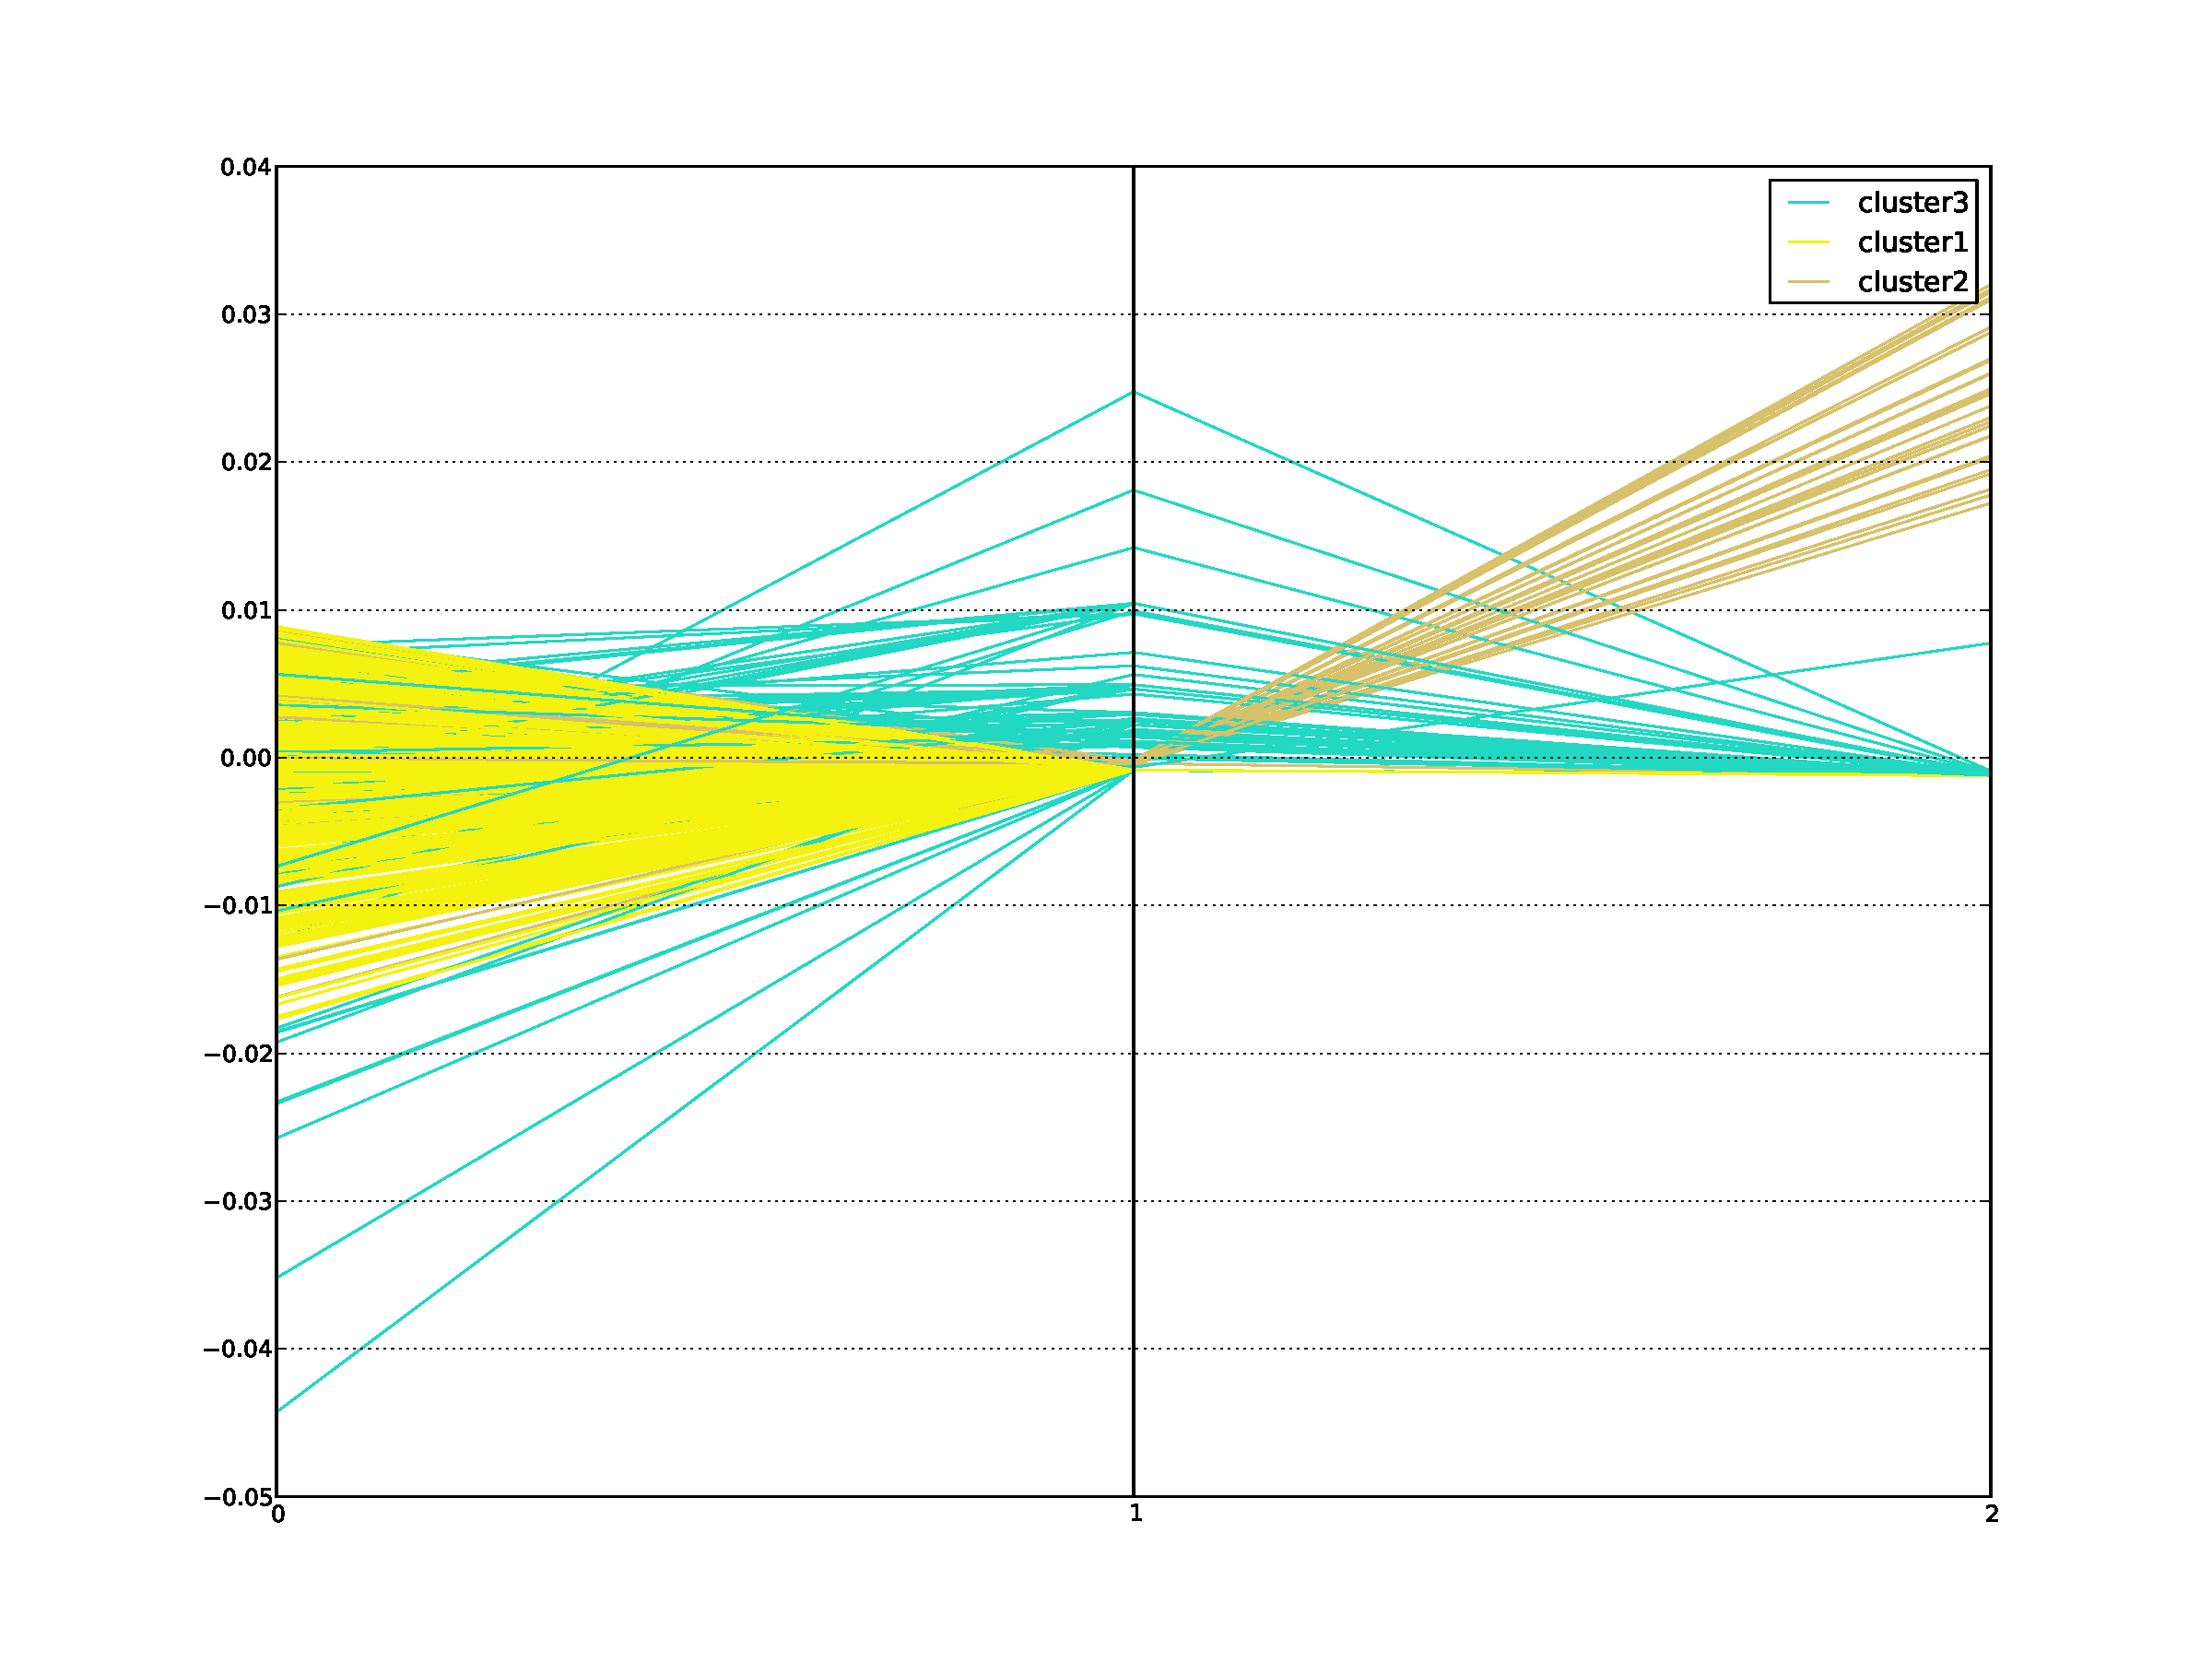
\includegraphics[width=3in]{part2/adult/parallel-ica-cluster.pdf}
    \caption{parallel plot ica cluster - adult\label{parallel-ica-cluster}}
\end{figure} 

\paragraph{RP}

Creating random projections of the dataset onto five components resulted in mixed behavior. The distribution of values for resulting features had significantly random and differing profiles. Clustering results using those features varied both in cluster concentrations and distribution of instances into each distribution. Over five separate runs of random projection and EM clustering, we see log likelihood figures between 30 and 50. These concentrations range above and below those achieved using the original 14 attributes. Run times for each experiment also varied significantly, ranging from 15 to 40 seconds. To compare, the same clustering task took 22 seconds on the original data.

The main issue with the random projection clustering results are with the distribution of instances across the identified clusters. Figure~\ref{rp-custer-dist-adult} shows distributions for each experiment run as well as from clustering on the original attributes. The distributions for remote projection runs show significant deviation, which indicates that EM and k-means clustering identified quite different cluster centroids for each projected dataset.

\begin{verbbox}
Cluster Distributions on Original Attributes

Clustered Instances
0      17815 ( 55%)
1       4160 ( 13%)
2      10586 ( 33%)


Cluster Distributions on Random Projections

Clustered Instances
0       7515 ( 23%)
1      20815 ( 64%)
2       4231 ( 13%)

Clustered Instances
0       8684 ( 27%)
1      16861 ( 52%)
2       7016 ( 22%)

Clustered Instances
0       2226 (  7%)
1       2005 (  6%)
2      28330 ( 87%)
\end{verbbox}

\begin{figure}[!htbp]
    \centering
    \theverbbox
    \caption{random projection cluster distributions - adult\label{rp-custer-dist-adult}}
\end{figure}


\paragraph{Information Gain Ratio}

The final attribute selection algorithm tested was a filter based on attributes with the best information gain ratio. This showed positive results in reducing dimensions in classification tasks. For clustering, the attributes with the top five gain ratio values were used in the clustering task (Figure~\ref{gain-adult}).

\begin{verbbox}
Search Method:
    Attribute ranking.

Attribute Evaluator (supervised, Class (nominal): 15 class):
    Gain Ratio feature evaluator

Ranked attributes:
 0.1876  11 capital-gain
 0.1165  12 capital-loss
 0.0854   6 marital-status
 0.0768   8 relationship
 0.0406  10 sex
\end{verbbox}
\normalsize

\begin{figure}[!htbp]
    \centering
    \theverbbox
    \caption{gain ratio selected attributes - adult\label{gain-adult}}
\end{figure}


The resulting clusters where not as distinguishable as those produced with PCA. Figure~\ref{parallel-gain-cluster} shows the resulting grouping after running EM clustering on the reduced dataset.

\begin{figure}[!htbp]
    \centering
    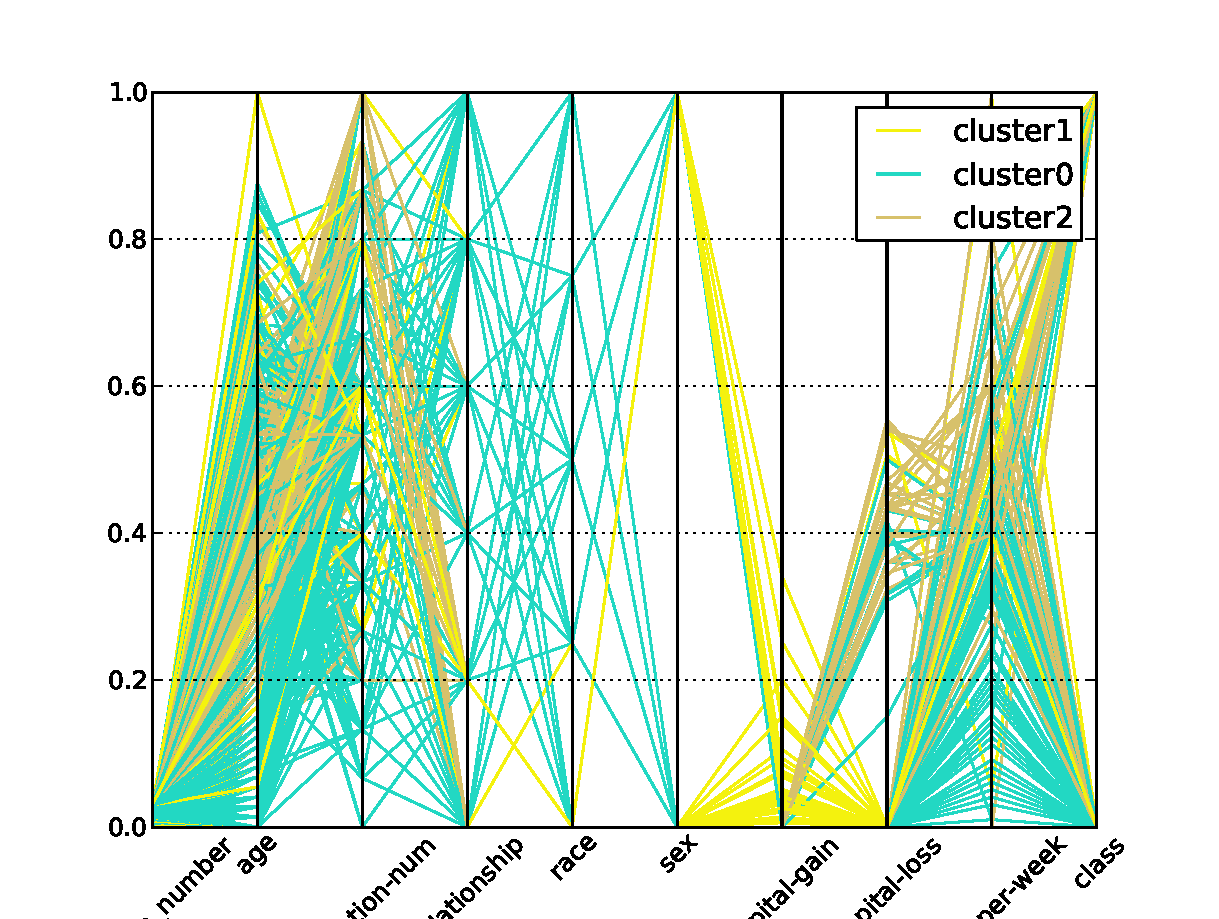
\includegraphics[width=3in]{part2/adult/parallel-gain-cluster.pdf}
    \caption{gain-ratio clusters - adult\label{parallel-gain-cluster}}
\end{figure} 

%Reproduce your clustering experiments, but on the data after you've run dimensionality reduction on it.



\subsection{Exploring Dataset 2: Iris}

The second dataset we will explore is the Iris dataset from UCI. This is a very well studied dataset with a small sample size, which should help in understanding the effects of our clustering and dimensionality reduction algorithms. The distribution of instances by their class label is shown in Figure~\ref{iris-parallel-class}. Visually, we see two groupings based on petal length and width. However, the data is labeled with three classes (species). Once of these classes matches perfectly with one of the natural groupings, which the other two fall clearly into the other. This can also be seen in many of the attribute scatter plots (Figure~\ref{iris-attr-scatter}).

\begin{figure}[!htbp]
    \centering
    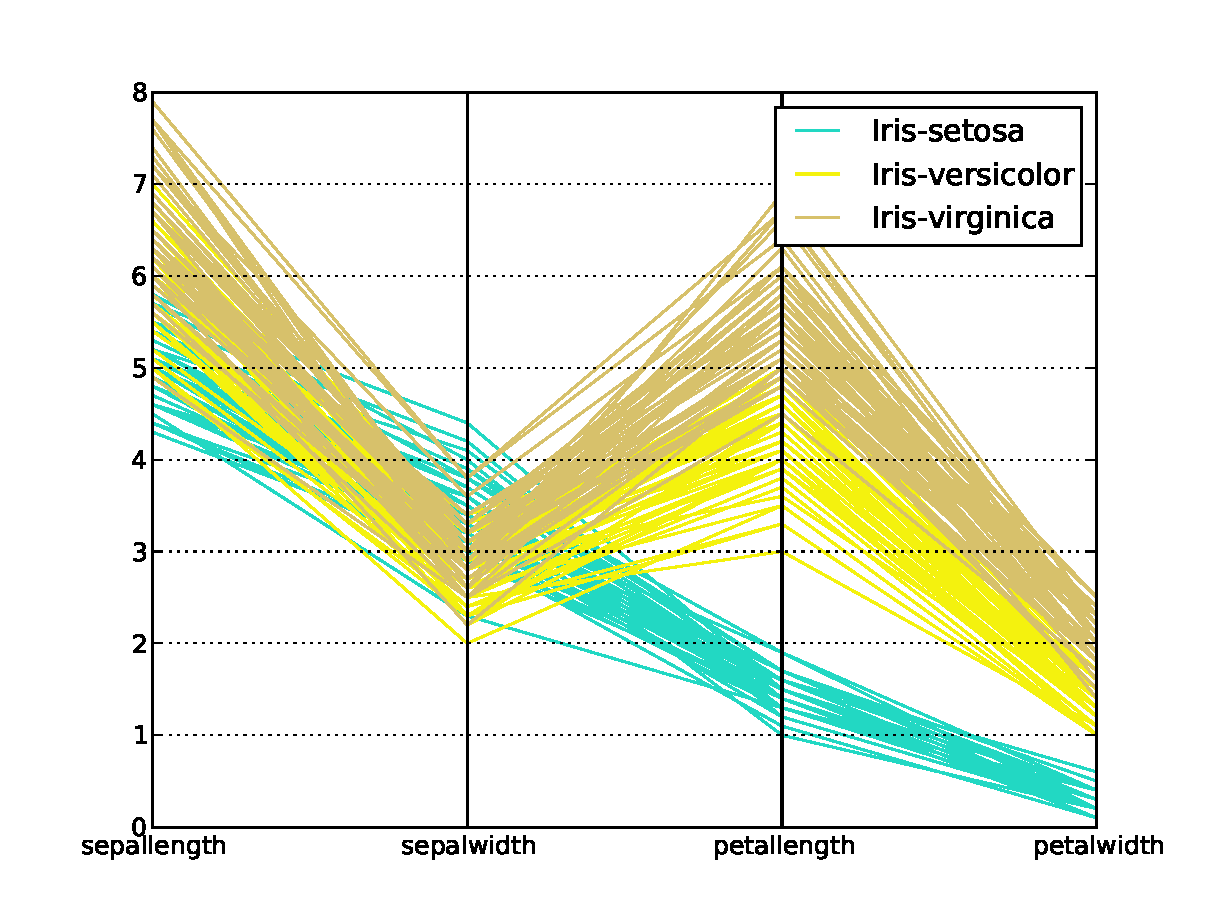
\includegraphics[width=3in]{part2/iris/parallel-class.pdf}
    \caption{dataset parallel plot - iris\label{iris-parallel-class}}
\end{figure} 

\begin{figure}[!htbp]
    \centering
    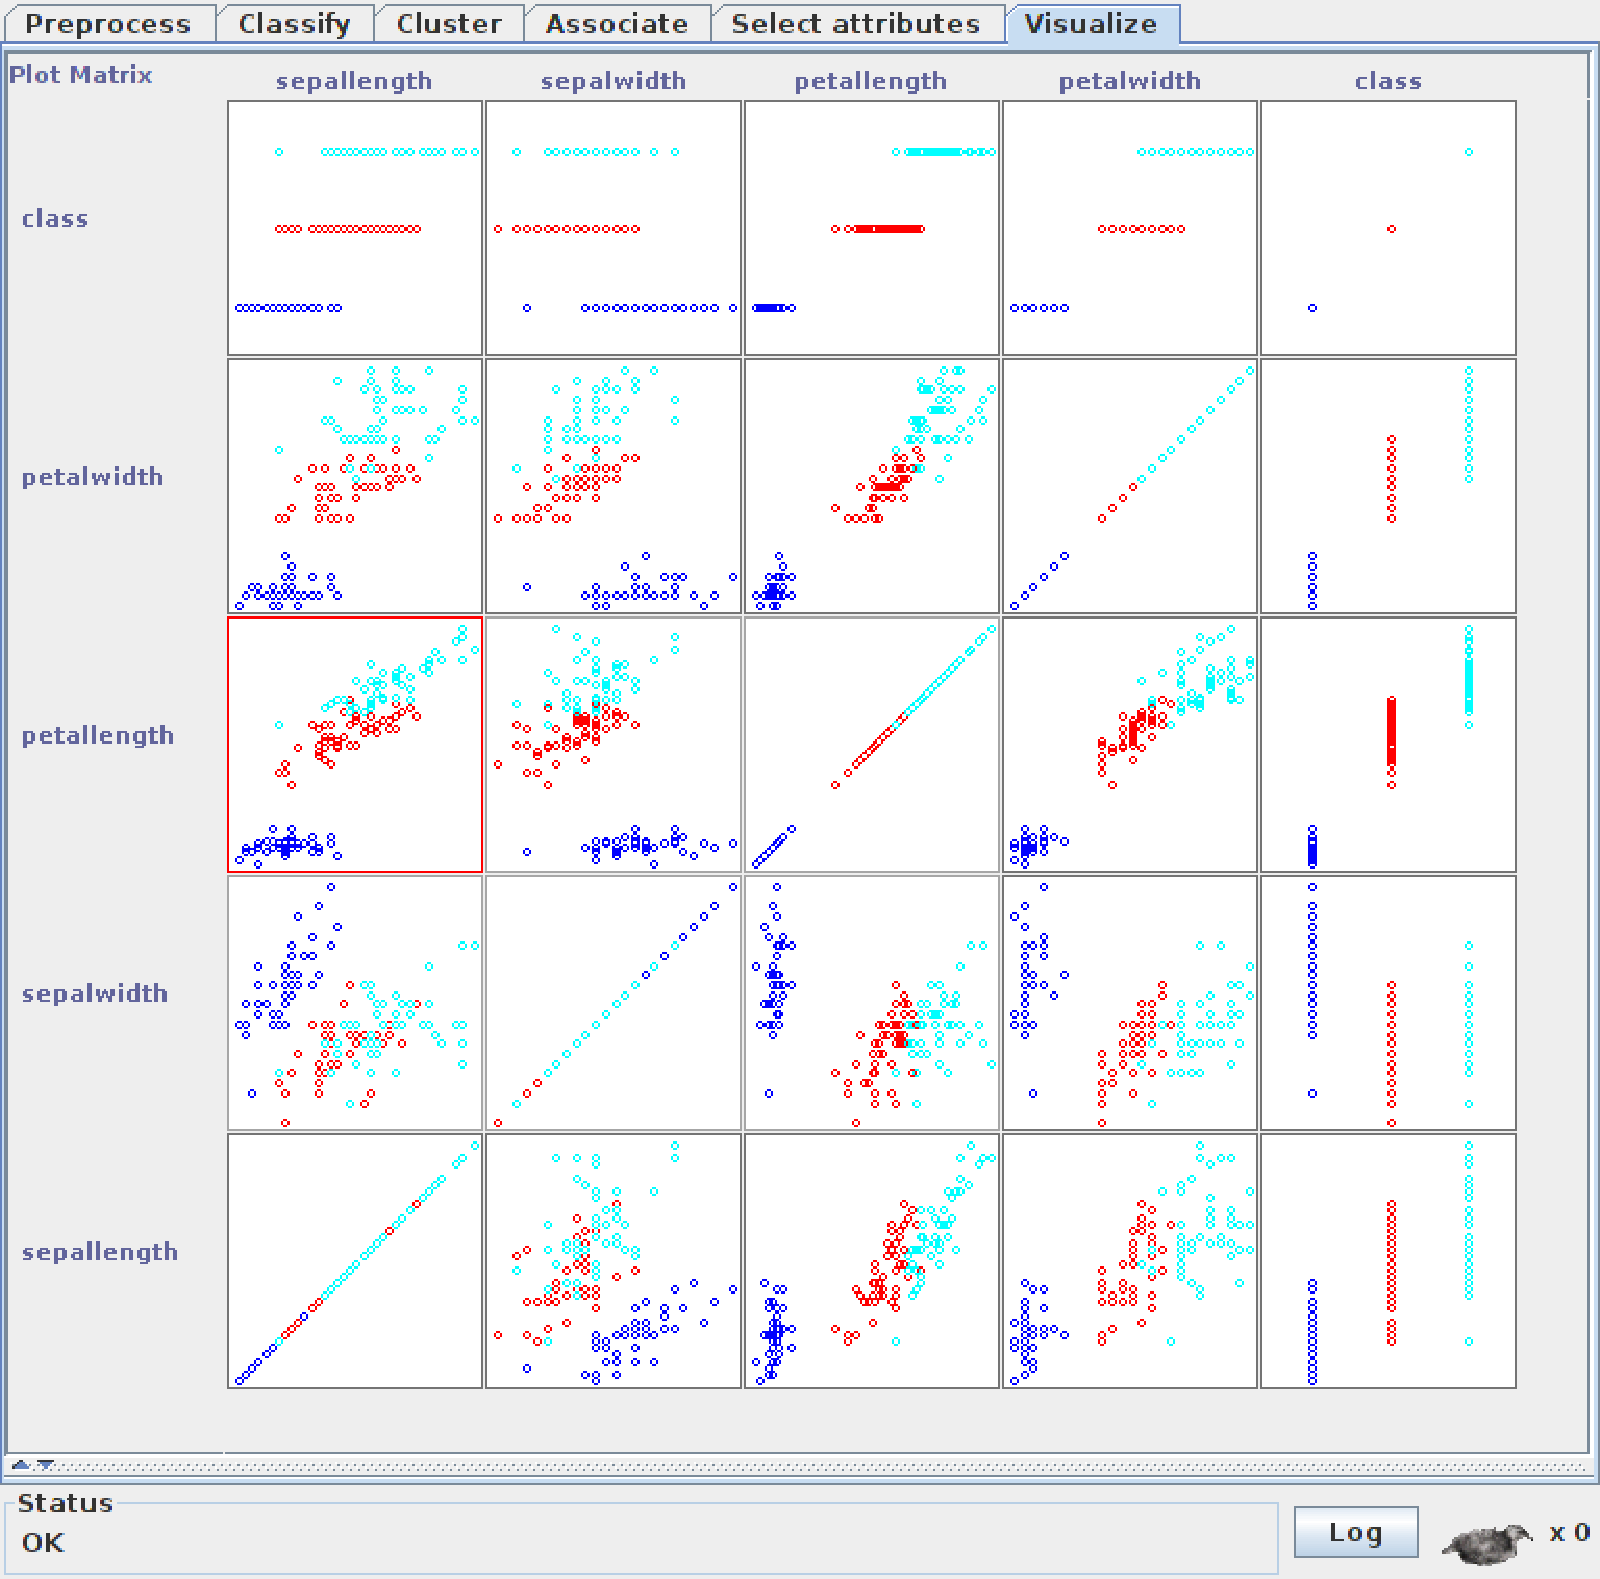
\includegraphics[width=3in]{part2/iris/attribute-scatter.pdf}
    \caption{attribute scatter plots - iris\label{iris-attr-scatter}}
\end{figure} 

\subsubsection{Clustering}

%Run the clustering algorithms on the data sets and describe what you see.

As with our first dataset, the EM clustering algorithm was run against the iris dataset with automatic determination of the number of clusters. According to this process, splitting the data into five clusters resulted in the lowest log likelihood value. However, as we can see from 

Form the results of k-means (Figure~\ref{kmeans-summary}) and EM (Figure~\ref{kmeans-summary}) clustering, three distinct profiles emerge from the data:

\paragraph{Cluster 1 - Young and poor}
\begin{itemize}[itemsep=1pt]
    \item Young (34)
    \item Less educated (9.8)
    \item Single (Never-married, Divorced, Separated, Widowed)
    \item Works less hours (37.5)
    \item Low income (<50k)
\end{itemize}

\paragraph{Cluster 2 - Older and experienced}
\begin{itemize}[itemsep=1pt]
    \item Older (43)
    \item More educated (12.5)
    \item Male
    \item High cap gain/loss (5000/475)
    \item Works more hours (44.8)
    \item High income (>50k)
\end{itemize}

\paragraph{Cluster 3 - Older blue collar}
\begin{itemize}[itemsep=1pt]
    \item Older (43)
    \item less educated (9.8)
    \item Currently Married
    \item Male
    \item Works medium hours (43)
    \item Low income (<50k)
\end{itemize}



\tiny
\begin{verbbox}
Running k-means

Within cluster sum of squared errors: 94691.74506148841
Missing values globally replaced with mean/mode

Cluster centroids:
                                     Cluster#
Attribute           Full Data               0              1              2
                      (32561)          (7243)        (14601)        (10717)
===========================================================================
age                   38.5816         43.6339        32.9471        42.8437
workclass             Private         Private        Private        Private
fnlwgt            189778.3665     187061.4272    192070.6165    188491.5931
education             HS-grad       Bachelors        HS-grad        HS-grad
education-num         10.0807         12.6281         9.8104         8.7273
marital-status        Married         Married  Never-married        Married
occupation     Prof-specialty  Prof-specialty   Adm-clerical   Craft-repair
relationship          Husband         Husband  Not-in-family        Husband
race                    White           White          White          White
sex                      Male            Male         Female           Male
capital-gain        1077.6488       3607.9214       269.1136       469.1444
capital-loss          87.3038        179.5659        50.7723        74.7204
hours-per-week        40.4375         45.0614        36.5254        42.6422
native-country  United-States   United-States  United-States  United-States
class                   <=50K            >50K          <=50K          <=50K
\end{verbbox}
\normalsize

\begin{figure}[!htbp]
    \centering
    \theverbbox
    \caption{k-means clustering results\label{kmeans-summary}}
\end{figure}


\scriptsize
\begin{verbbox}
EM
==

Number of clusters selected by cross validation: 3


                     Cluster
Attribute                  0           1           2
                      (0.53)      (0.18)      (0.28)
=====================================================
age
  mean                34.4071     43.6058     43.2169
  std. dev.           13.4275     11.5698     12.6479

education-num
  mean                 9.8028     12.4534        9.07
  std. dev.            2.3915      2.2579      2.1192

relationship
   Not-in-family    7417.5347    732.4946    157.9707
   Husband             6.5078    4459.228   8730.2642
   Wife             1044.7802     372.591    153.6288
   Own-child         4842.923     166.438      61.639
   Unmarried        3189.2812    193.3051     66.4137
   Other-relative    899.9176     41.2378     42.8447
  [total]          17400.9445   5965.2944   9212.7611
sex
   Male             7798.0266   5069.9658   8925.0076
   Female           9598.9179    891.3286    283.7535
  [total]          17396.9445   5961.2944   9208.7611
capital-gain
  mean                  4.065   5506.3843     239.438
  std. dev.           60.7467  16515.2342    873.4603

capital-loss
  mean                      0    475.4836      0.9942
  std. dev.          402.9602    837.7166     25.1187

hours-per-week
  mean                37.5504     44.8544     43.0332
  std. dev.           12.1264     11.7279     11.7133

class
   <=50K           16342.7922   1688.2196   6691.9882
   >50K             1054.1523   4273.0749   2516.7729
  [total]          17396.9445   5961.2944   9208.7611


Time taken to build model (full training data) : 395.06 seconds

=== Model and evaluation on training set ===

Clustered Instances

0      17815 ( 55%)
1       4160 ( 13%)
2      10586 ( 33%)

Log likelihood: -46.47694
\end{verbbox}
\normalsize

\begin{figure}[!htbp]
    \centering
    \theverbbox
    \caption{subset of EM clustering results\label{em-summary}}
\end{figure}

Visualizing the samples based on their cluster assignments shows a somewhat clearer distinction than their class assignment plots. Figures~\ref{adult-attr-cluster}~and~\ref{adult-parallel-cluster} show these distributions. Figure~\ref{adult-parallel-cluster} provides a better picture of the groupings. We can see in this visualization how younger individuals cluster in their marital-status, relationship, capital gains, hours-per-week, and income class. Likewise, we see the profile pattern for the older, experienced, group (yellow). These individuals share the attributes of being older, having higher education levels, higher capital-gains, and more hours-per-week. It should be noted that although these grouping are clear enough to see upon examination, they do not stand out with complete distinctiveness. There is a significant amount of noise in the data, which many samples that do not conform the to complete set of common profile attributes.

\begin{figure}[!htbp]
    \centering
    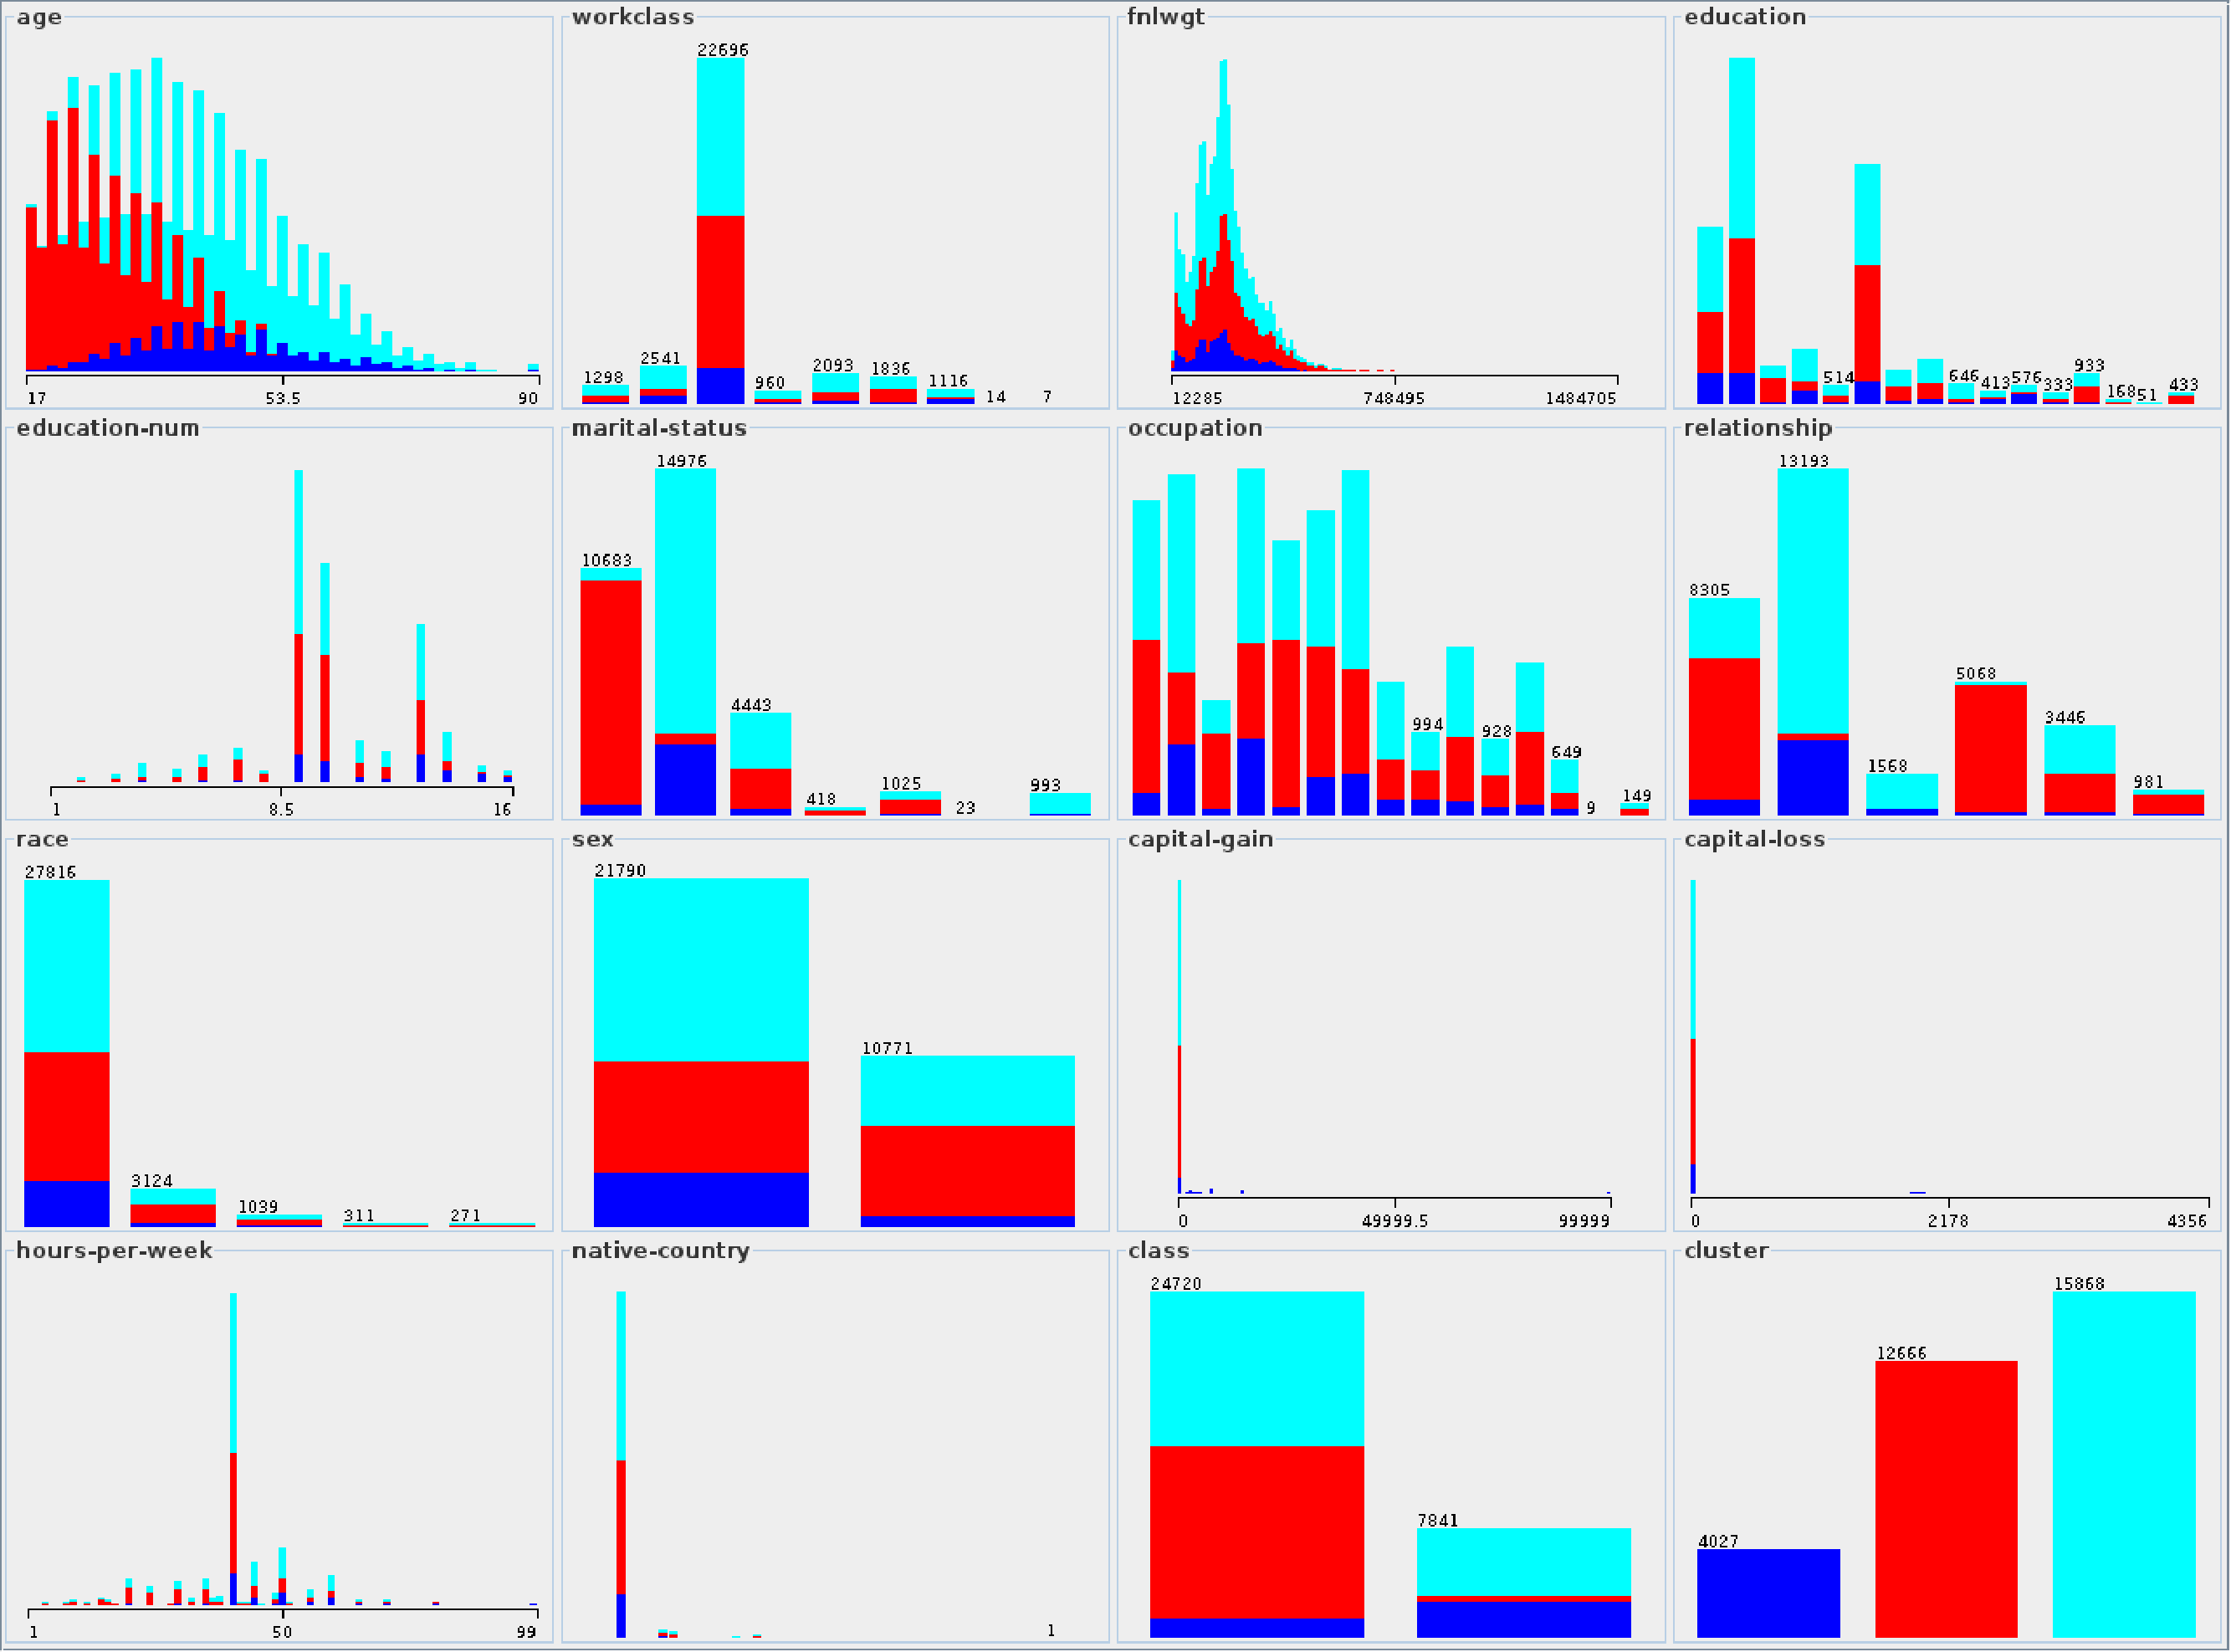
\includegraphics[width=3in]{part2/adult/attr-cluster.pdf}
    \caption{dataset attributes by cluster - adult\label{adult-attr-cluster}}
\end{figure} 

\begin{figure}[!htbp]
    \centering
    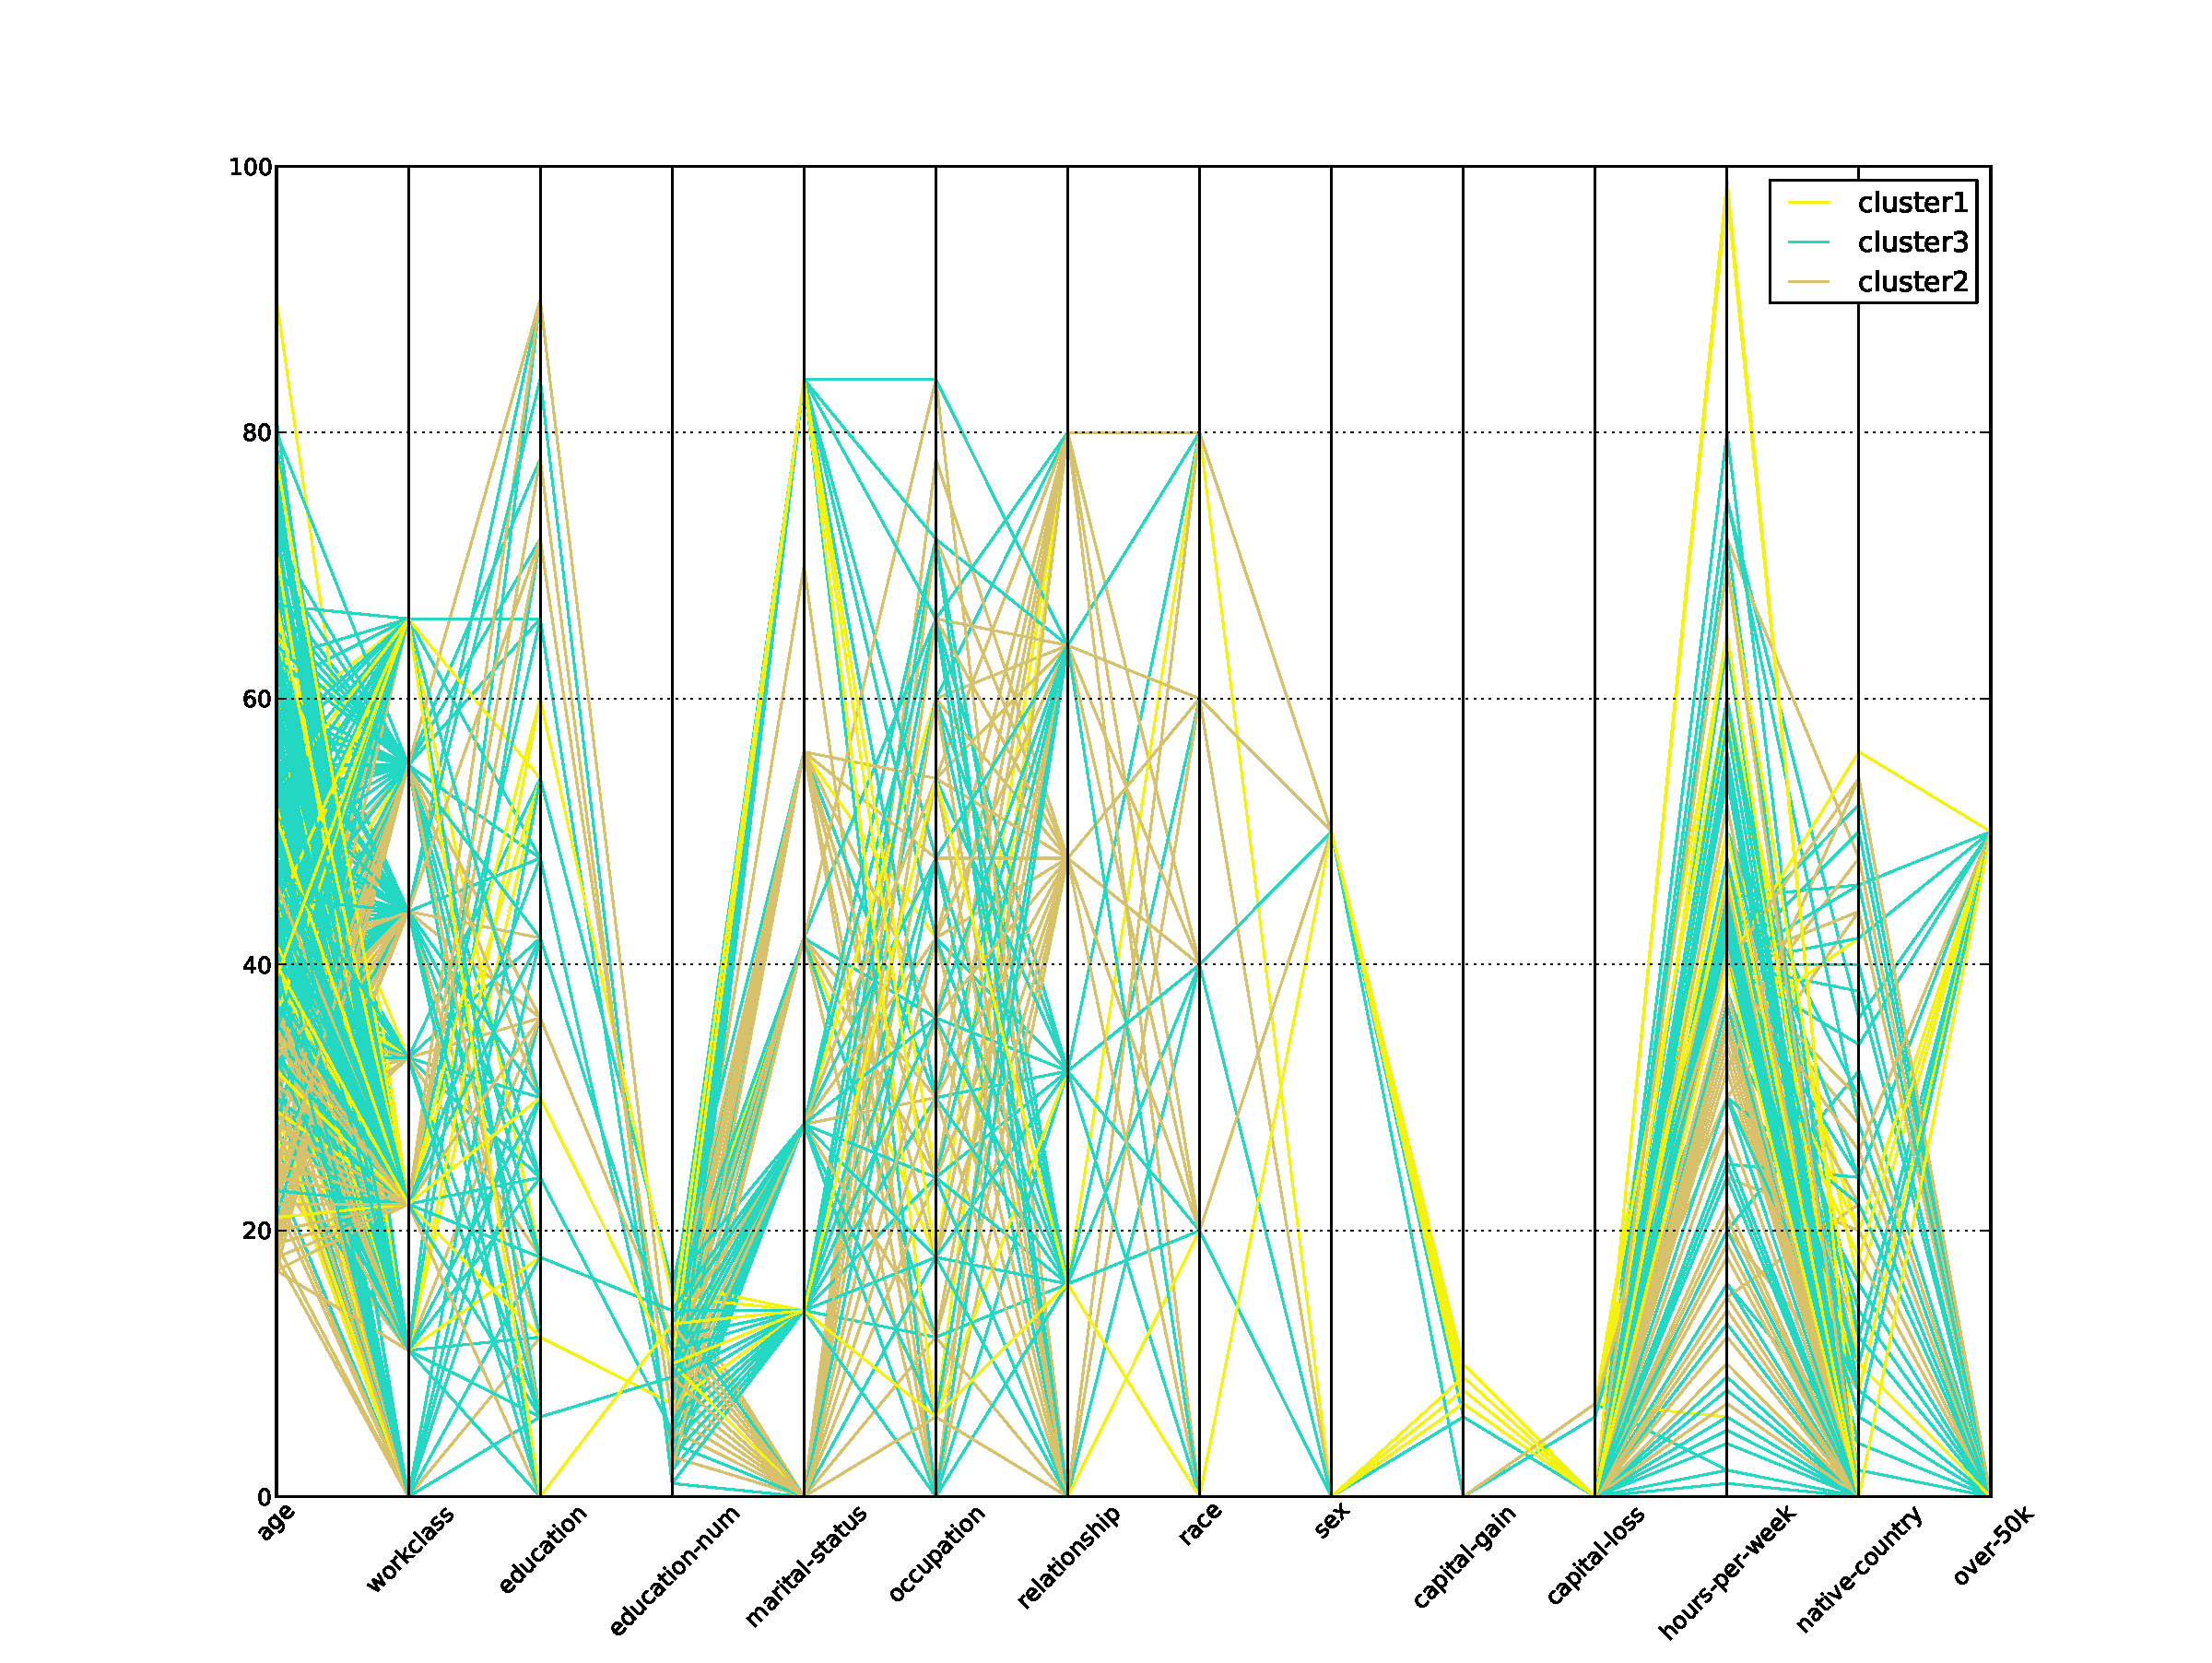
\includegraphics[width=3in]{part2/adult/parallel-cluster.pdf}
    \caption{dataset parallel plot by cluster - adult\label{adult-parallel-cluster}}
\end{figure} 


\subsubsection{Clustering on Dimensionally Reduced Dataset}

%Apply the dimensionality reduction algorithms to the two datasets and describe what you see.

\paragraph{PCA}
Running PCA on the Adult dataset results in features with the characteristics shown in Figure~\ref{pca-adult}. The first few principle components capture 11\% of the dataset variance. The distribution of eigenvalues shows that the roughly the first five components distinguish themselves in regards to their contribution to the overall variance.


\begin{verbbox}
eigenvalue  proportion  cumulative
4.13178     0.03861     0.03861
2.89985     0.0271      0.06572
2.5952      0.02425     0.08997
2.42699     0.02268     0.11265
2.23305     0.02087     0.13352
1.90511     0.0178      0.15133
1.63445     0.01528     0.1666 
1.5871      0.01483     0.18143
1.49286     0.01395     0.19539
1.42284     0.0133      0.20868
1.37072     0.01281     0.22149
1.31255     0.01227     0.23376
1.29281     0.01208     0.24584
1.2507      0.01169     0.25753
1.23304     0.01152     0.26906
1.21991     0.0114      0.28046
1.19888     0.0112      0.29166
1.17351     0.01097     0.30263
1.16087     0.01085     0.31348
1.14374     0.01069     0.32417
1.12887     0.01055     0.33472
1.12004     0.01047     0.34519
1.11544     0.01042     0.35561
1.09716     0.01025     0.36586
1.09448     0.01023     0.37609
1.08928     0.01018     0.38627
1.08335     0.01012     0.3964 
1.07809     0.01008     0.40647
1.06987     0.01        0.41647
\end{verbbox}

\begin{figure}[!htbp]
    \centering
    \theverbbox
    \caption{PCA eigenvalues - adult\label{pca-adult}}
\end{figure}

Clustering on the first five components from our resulting PCA features creates clusters with much clearer distinctions than with the original 14 attributes. Figure~\ref{pca-cluster-scatter} shows the cluster assignments based on only the first component (spread out over the instance numbers). With just this single attribute, we can see a clearer segregation of our three clusters. Log likelihood from EM clustering came out to -9.15, which is significantly higher than -46.5 achieved with the original attributes. K-means clustering resulted in a similar plot, and a sum of squared errors within each cluster of 2,620.

\begin{figure}[!htbp]
    \centering
    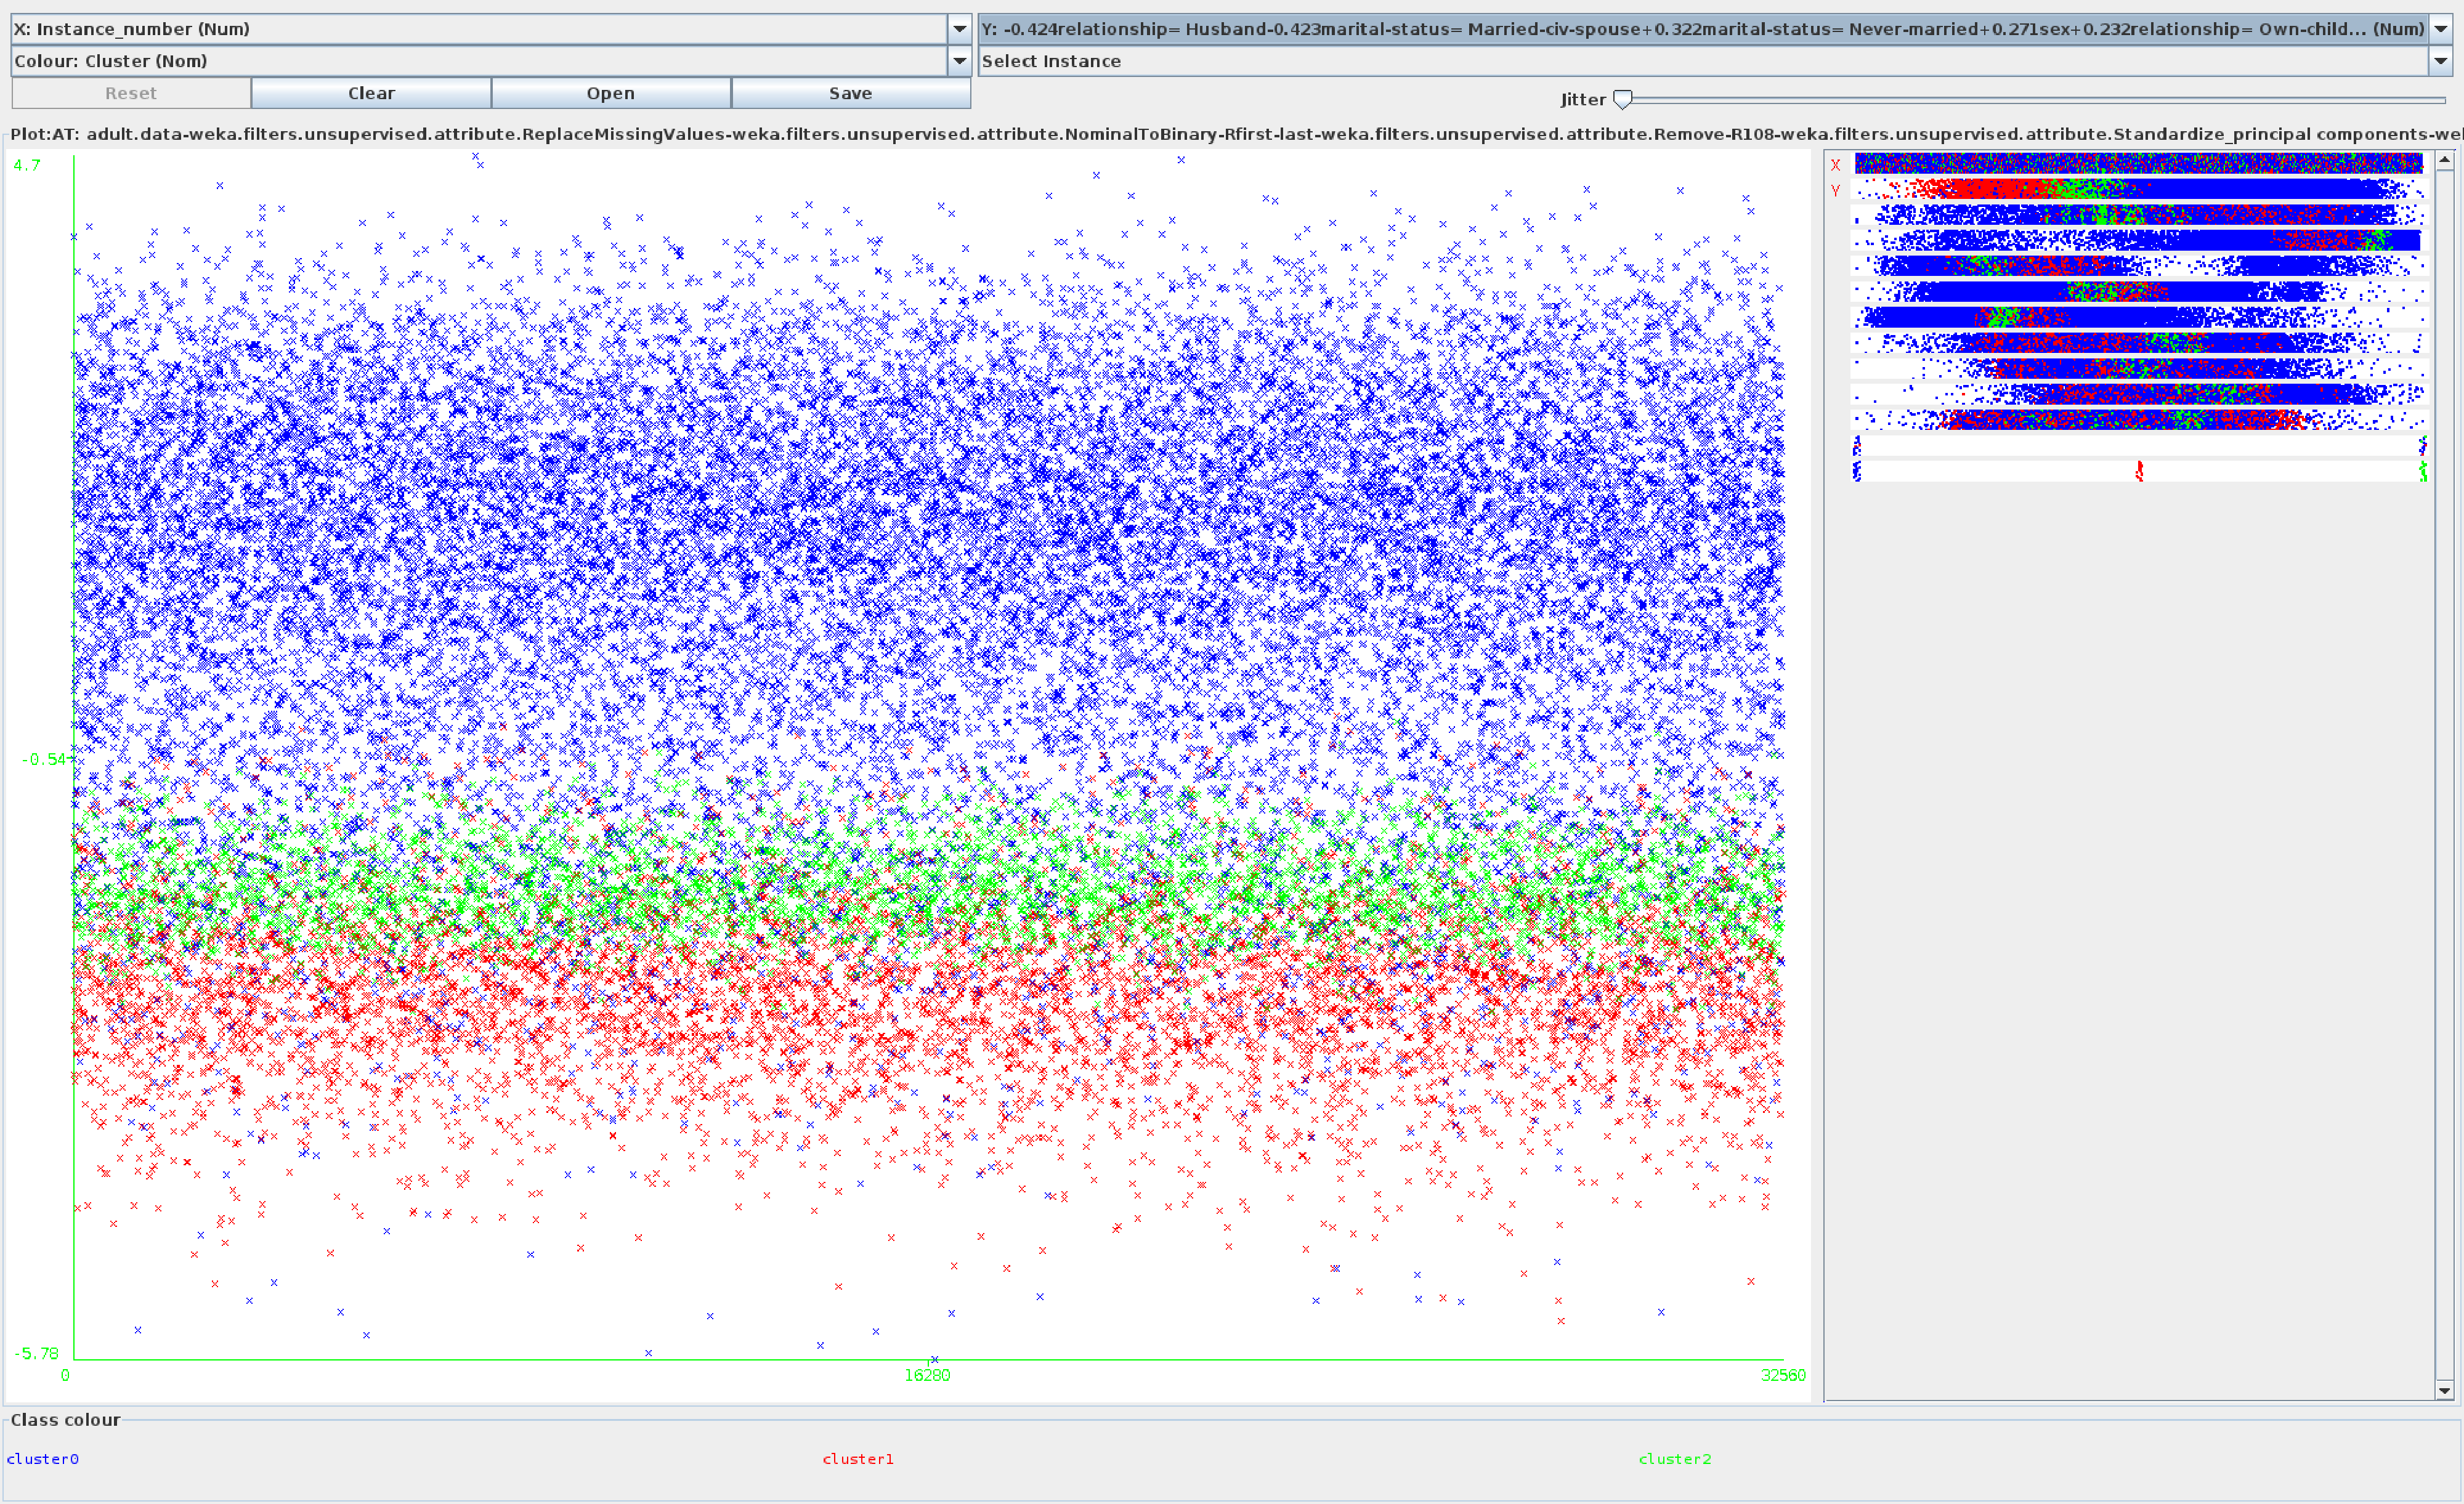
\includegraphics[width=3in]{part2/adult/pca-cluster-scatter.pdf}
    \caption{pca clusters on fist component - adult\label{pca-cluster-scatter}}
\end{figure} 


\paragraph{ICA}

Running independent component analysis on the dataset required a decision regarding the number of independent features to output. Without foreknowledge, experimentation was necessary to find an appropriate number of components. This was accomplished by iterating up to the original number of features, running ICA with that number of target components, and comparing the resulting kurtosis to determine how well ICA was able to pull independent features from the mixed uniform distribution. The intuition begin that a set of features with a high absolute biased kurtosis (zeroed at normal distribution), would indicate significant, independent, contributing features.

The result of this experiments can be seen in Figure~\ref{ica-stats-adult}. From this data we can make an informed decision regarding how many components to output from ICA for use in our clustering task. 

\tiny
\begin{verbbox}
  n  min/max                  mean            var         skew    kurtosis
---  ------------------  ---------  -------------  -----------  ----------
  1  (6.217, 6.21775)     6.21775      0           0             -3
  2  (35.31, 45.3218)    40.3204      50.0296      2.15814e-15   -2
  3  (6.214, 154.845)    60.4781    6729.09        0.683477      -1.5
  4  (0.2694, 155.271)   45.5331    5423.68        1.11028       -0.703042
  5  (0.2143, 155.314)   37.0787    4428.31        1.45134        0.180383
  6  (1.399, 155.273)    35.3957    3554.86        1.67272        0.985259
  7  (0.222, 155.400)    30.6465    3132.59        1.90229        1.84921
  8  (0.0771, 155.355)   26.9649    2793.2         2.11254        2.72931
  9  (0.2083, 155.775)   24.3725    2519.2         2.31297        3.63809
 10  (0.3312, 155.651)   22.0006    2291.2         2.49168        4.53032
 11  (0.4255, 155.747)   20.3085    2095.81        2.66496        5.44675
 12  (0.1315, 155.606)   19.2382    1914.82        2.8292         6.37344
 13  (0.1338, 155.619)   20.6722    1781.69        2.78072        6.45888
 14  (0.6387, 0.817448)   0.721304     0.00240131  0.167194      -0.364713
\end{verbbox}
\normalsize

\begin{figure}[!htbp]
    \centering
    \theverbbox
    \caption{ICA kurtosis stats by number of features - adult\label{ica-stats-adult}}
\end{figure}

Reducing to three components resulted in kurtosis of [6.2, 154.8, 20.3]. This signifies three, non-normally distributed, independent features. Performing EM and k-means clustering on the ICA filtered dataset resulted in a tight clusters (EM log likelihood: 23.5, k-means SSE: 270.4). Visualization of these clusters is shown in Figure~\ref{parallel-ica-cluster}. These show much more distinct groupings than with the original data. The EM clustering task took 12 seconds with these features, which is nearly half the time it required to process the original 14 features.

\begin{figure}[!htbp]
    \centering
    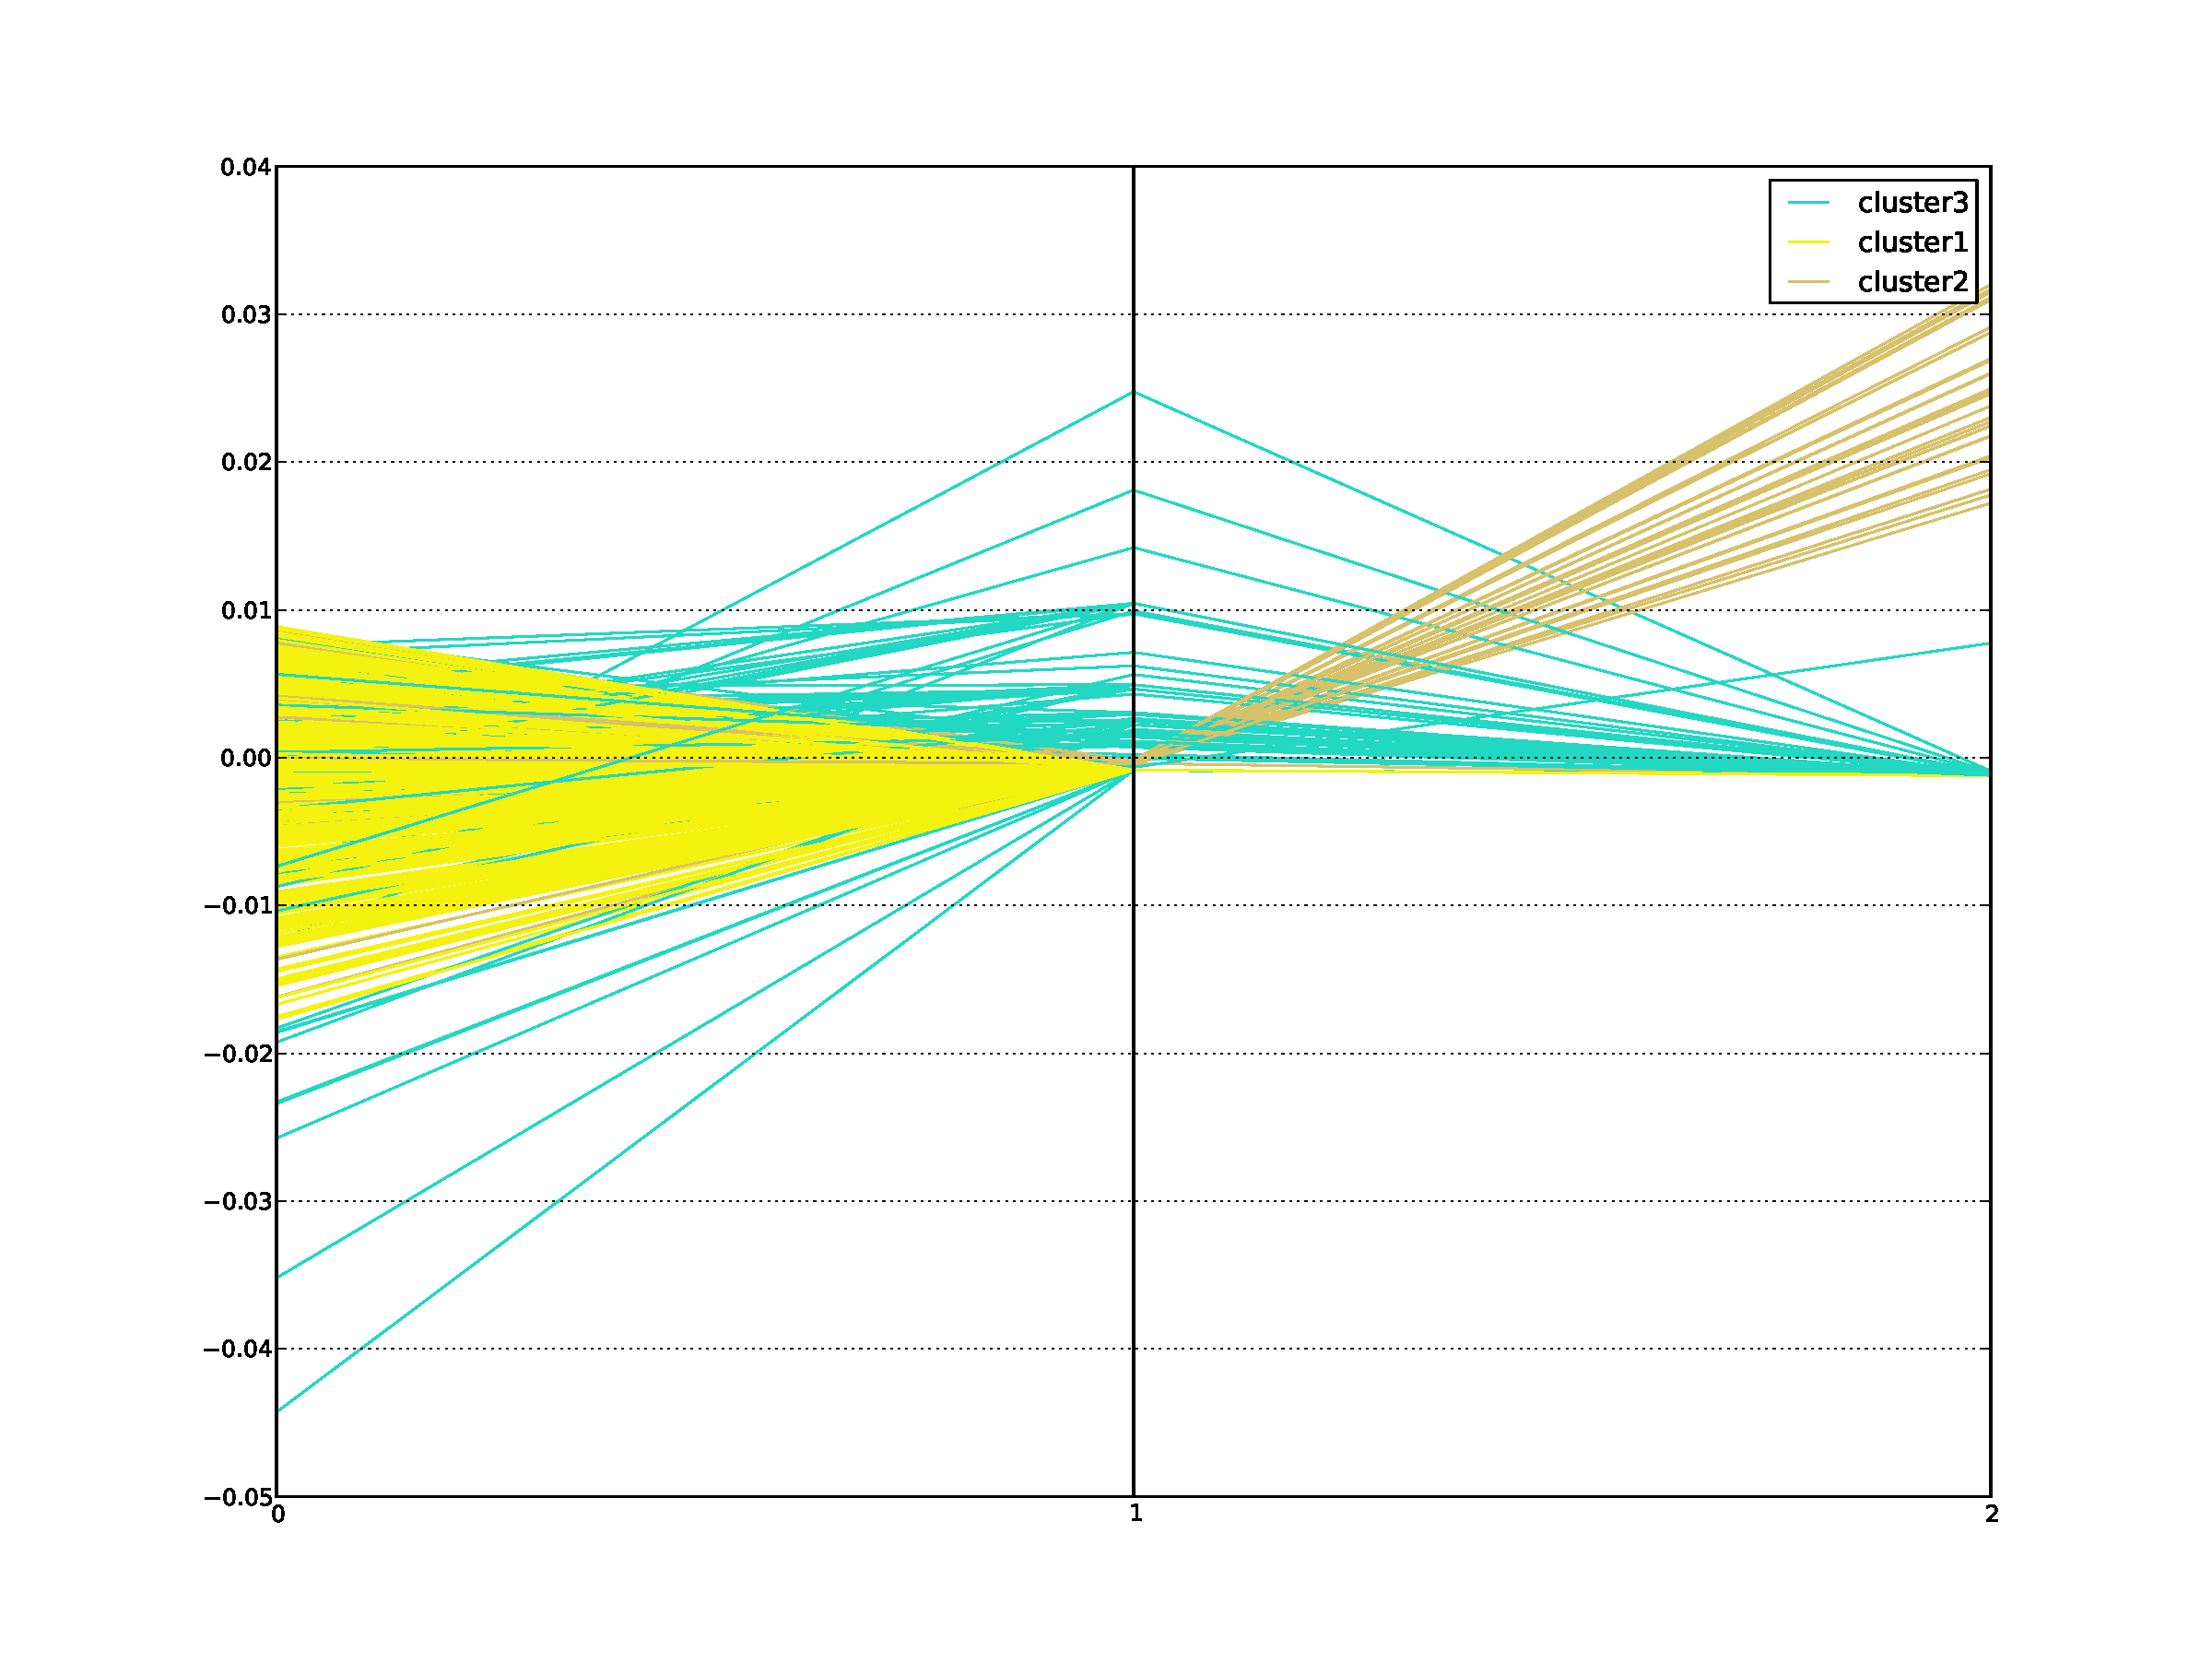
\includegraphics[width=3in]{part2/adult/parallel-ica-cluster.pdf}
    \caption{parallel plot ica cluster - adult\label{parallel-ica-cluster}}
\end{figure} 

\paragraph{RP}

Creating random projections of the dataset onto five components resulted in mixed behavior. The distribution of values for resulting features had significantly random and differing profiles. Clustering results using those features varied both in cluster concentrations and distribution of instances into each distribution. Over five separate runs of random projection and EM clustering, we see log likelihood figures between 30 and 50. These concentrations range above and below those achieved using the original 14 attributes. Run times for each experiment also varied significantly, ranging from 15 to 40 seconds. To compare, the same clustering task took 22 seconds on the original data.

The main issue with the random projection clustering results are with the distribution of instances across the identified clusters. Figure~\ref{rp-custer-dist-adult} shows distributions for each experiment run as well as from clustering on the original attributes. The distributions for remote projection runs show significant deviation, which indicates that EM and k-means clustering identified quite different cluster centroids for each projected dataset.

\begin{verbbox}
Cluster Distributions on Original Attributes

Clustered Instances
0      17815 ( 55%)
1       4160 ( 13%)
2      10586 ( 33%)


Cluster Distributions on Random Projections

Clustered Instances
0       7515 ( 23%)
1      20815 ( 64%)
2       4231 ( 13%)

Clustered Instances
0       8684 ( 27%)
1      16861 ( 52%)
2       7016 ( 22%)

Clustered Instances
0       2226 (  7%)
1       2005 (  6%)
2      28330 ( 87%)
\end{verbbox}

\begin{figure}[!htbp]
    \centering
    \theverbbox
    \caption{random projection cluster distributions - adult\label{rp-custer-dist-adult}}
\end{figure}


\paragraph{Information Gain Ratio}

The final attribute selection algorithm tested was a filter based on attributes with the best information gain ratio. This showed positive results in reducing dimensions in classification tasks. For clustering, the attributes with the top five gain ratio values were used in the clustering task (Figure~\ref{gain-adult}).

\begin{verbbox}
Search Method:
    Attribute ranking.

Attribute Evaluator (supervised, Class (nominal): 15 class):
    Gain Ratio feature evaluator

Ranked attributes:
 0.1876  11 capital-gain
 0.1165  12 capital-loss
 0.0854   6 marital-status
 0.0768   8 relationship
 0.0406  10 sex
\end{verbbox}
\normalsize

\begin{figure}[!htbp]
    \centering
    \theverbbox
    \caption{gain ratio selected attributes - adult\label{gain-adult}}
\end{figure}


The resulting clusters where not as distinguishable as those produced with PCA. Figure~\ref{parallel-gain-cluster} shows the resulting grouping after running EM clustering on the reduced dataset.

\begin{figure}[!htbp]
    \centering
    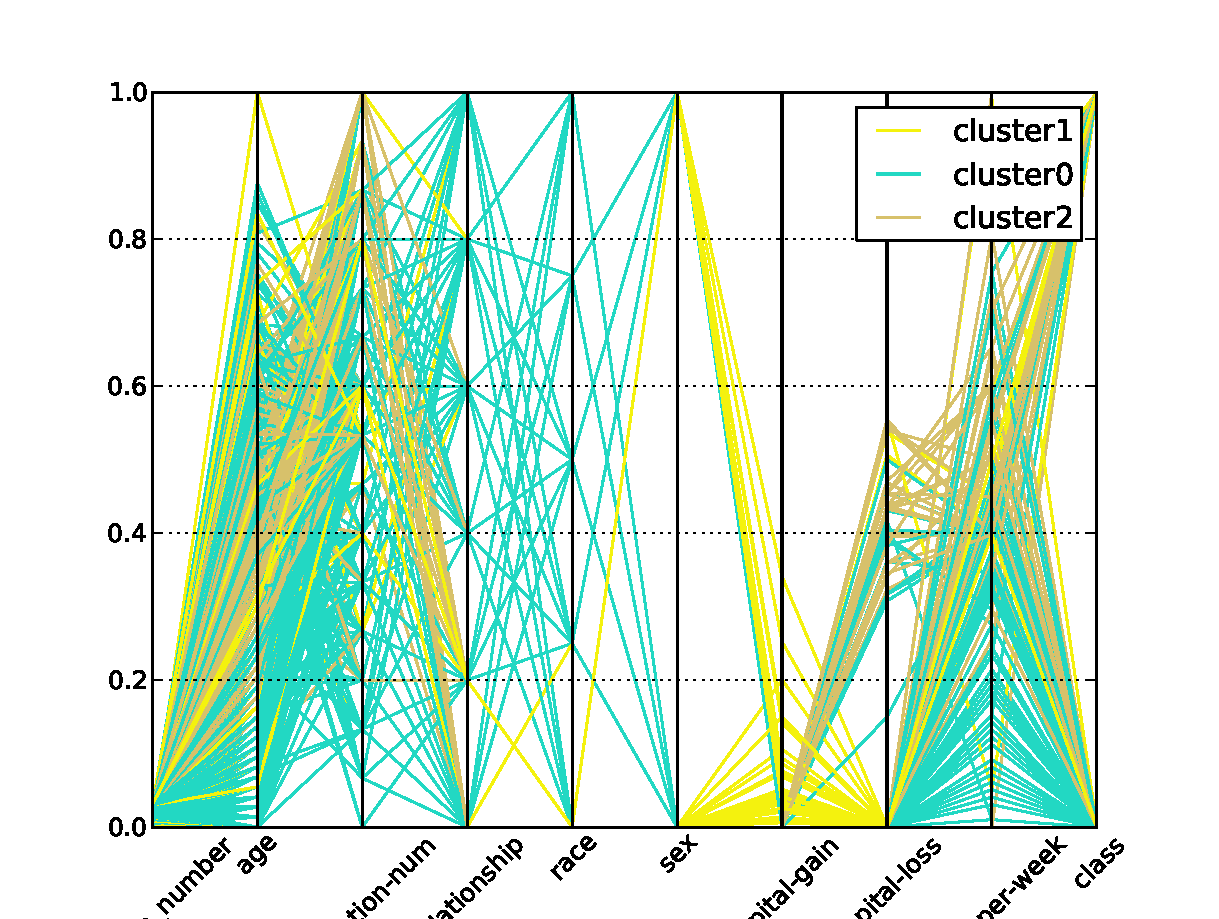
\includegraphics[width=3in]{part2/adult/parallel-gain-cluster.pdf}
    \caption{gain-ratio clusters - adult\label{parallel-gain-cluster}}
\end{figure} 

%Reproduce your clustering experiments, but on the data after you've run dimensionality reduction on it.


\subsection{Neural Network Training}

Using the Adult dataset, a neural network was trained with three sample inputs. First, the network was trained with the original features. The results of this are shown in Figure~\ref{ann-summary-original}. The main issue we see here is the amount of time it took to train this network. Since many of the 14 attributes are nominal, the dataset was processed with a nominal to binary attribute filter. This increased the number of attributes to 107. With this many input nodes, our neural network took significantly longer to train.


\tiny
\begin{verbbox}
Time taken to build model: 115.76 seconds

=== Evaluation on test split ===
=== Summary ===

Correctly Classified Instances        9390               84.8162 %
Incorrectly Classified Instances      1681               15.1838 %
Kappa statistic                          0.5291
Mean absolute error                      0.1558
Root mean squared error                  0.3563
Relative absolute error                 42.7879 %
Root relative squared error             84.0266 %
Total Number of Instances            11071     

=== Detailed Accuracy By Class ===

       TP Rate   FP Rate   Precision   Recall  F-Measure   ROC Area  Class
         0.946     0.472      0.867     0.946     0.905      0.89      <=50K
         0.528     0.054      0.752     0.528     0.62       0.895     >50K
WAvg.    0.848     0.374      0.84      0.848     0.838      0.891

=== Confusion Matrix ===

    a    b   <-- classified as
 8016  454 |    a =  <=50K
 1227 1374 |    b =  >50K
\end{verbbox}
\normalsize

\begin{figure}[!htbp]
    \centering
    \theverbbox
    \caption{ANN results with original attributes - adult\label{ann-summary-original}}
\end{figure}


\subsubsection{Training on Dimensionally Reduced Dataset}
%Apply the dimensionality reduction algorithms to one of your datasets from assignment #1 (if you've reused the datasets from assignment #1 to do experiments 1-3 above then you've already done this) and rerun your neural network learner on the newly projected data.

Using the five principle components identified earlier, a new neural network was created. The resulting classifier performed slightly poorer than the first network. The full results are shown in Figure~\ref{ann-summary-pca}. The weighted f-score was slightly lower at 0.822. However, the time required to train this network was an order of magnitude less than with the original attributes (11 seconds).


\tiny
\begin{verbbox}
=== Summary ===

Correctly Classified Instances       10400               82.7894 %
Incorrectly Classified Instances      2162               17.2106 %
Kappa statistic                          0.5057
Mean absolute error                      0.2382
Root mean squared error                  0.3404
Total Number of Instances            12562     

=== Detailed Accuracy By Class ===

       TP Rate   FP Rate   Precision   Recall  F-Measure   ROC Area  Class
         0.915     0.439      0.865     0.915     0.889      0.885     <=50K
         0.561     0.085      0.681     0.561     0.615      0.885     >50K
WAvg.    0.828     0.352      0.82      0.828     0.822      0.885

=== Confusion Matrix ===

    a    b   <-- classified as
 8672  809 |    a =  <=50K
 1353 1728 |    b =  >50K
\end{verbbox}
\normalsize

\begin{figure}[!htbp]
    \centering
    \theverbbox
    \caption{ANN results with PCA attributes\label{ann-summary-pca}}
\end{figure}



\subsubsection{Training with Clusters as Features}

Using the cluster labels found from running the EM algorithm, we see that these new features work well as inputs for our neural network. Figure~\ref{ann-cluster-weights} shows that only one of the original attributes contributed more to the classification task than membership in one of the three clusters. 


\scriptsize
\begin{verbbox}
=== Classifier model (full training set) ===

Sigmoid Node 0
    Inputs    Weights
    Threshold    -17.01722606012109
    Attrib age    -0.04311914552721472
    Attrib fnlwgt    -1.100932504395319
    Attrib education-num    -3.0179209181138433
    Attrib capital-gain    -22.05996366406373
    Attrib capital-loss    -2.6552854980340603
    Attrib hours-per-week    -1.9397990427724914
    Attrib cluster=cluster1    5.810438640239912
    Attrib cluster=cluster2    6.456682699425463
    Attrib cluster=cluster3    4.838382453840594
Sigmoid Node 1
    Inputs    Weights
    Threshold    17.03124036918239
    Attrib age    0.043119145527213236
    Attrib fnlwgt    1.1009325043953322
    Attrib education-num    3.017920918113866
    Attrib capital-gain    22.05996366406516
    Attrib capital-loss    2.6552854980341793
    Attrib hours-per-week    1.939799042772536
    Attrib cluster=cluster1    -5.796424331180166
    Attrib cluster=cluster2    -6.442668390365682
    Attrib cluster=cluster3    -4.824368144780805
Class  <=50K
    Input
    Node 0
Class  >50K
    Input
    Node 1
\end{verbbox}
\normalsize

\begin{figure}[!htbp]
    \centering
    \theverbbox
    \caption{ANN weights with cluster input nodes\label{ann-cluster-weights}}
\end{figure}

With these new features, we were able to filter most of the remaining attributes without affecting the accuracy of the classifier. The neural network, trained on nine attributes including three for cluster membership, resulted in a weighted f-score of 0.824. The original dataset included 107 attributes (mainly due to nominal to binary filtering). That network resulted in an f-score of 8.38 and required 10 times as long to train.


%Apply the clustering algorithms to the same dataset to which you just applied the dimensionality reduction algorithms (you've probably already done this), treating the clusters as if they were new features. In other words, treat the clustering algorithms as if they were dimensionality reduction algorithms. Again, rerun your neural network learner on the newly projected data.






\begin{thebibliography}{10}

\bibitem{Bache+Lichman:2013}
K. Bache and M. Lichman
\newblock UCI Machine Learning Repository
\newblock 2013
\newblock http://archive.ics.uci.edu/ml
\newblock University of California, Irvine, School of Information and Computer Sciences

%\bibitem{Zhong:Osteo}
%L.~Zhong, D.~El-Daye, B.~Kaufman, N.~Tobaoda, T.~Mohamed, and M.~Liebschner.
%\newblock Osteoconduct: Wireless body-area communication based on bone
  %conduction.
%\newblock In {\em in Proc. Int. Conf. Body Area Networks (BodyNets)}, June
  %2007.

\end{thebibliography}
\end{document}
